\documentclass[a4paper,12pt]{article} 
\usepackage{multicol} 
% ---------- 第一步：页面布局/基础配置（最先加载） ----------
\usepackage{geometry}
\geometry{left=1in,right=0.75in,top=1in,bottom=1in}
\usepackage{microtype} % 更好的微排版

% ---------- 第二步：编码/字体基础（必须在字体包前） ----------
\usepackage[T1]{fontenc} % 输出字体编码
\usepackage[utf8]{inputenc} % 输入字符编码

% ---------- 第三步：核心字体包（newtx必须紧跟编码包） ----------
\usepackage{newtxtext} % Times西文（优先级最高，先加载）
\usepackage{amsmath, amssymb, amsthm} % 数学公式
\usepackage{newtxmath} % Times数学（依赖newtxtext）

%----------- 数学相关包 ---------------------------------------

\usepackage{mathtools}  % 改进 amsmath
                        % % 1. 更灵活的公式对齐（解决amsmath的小缺陷）
                        % \begin{align*}
                        % f(x) &= x^2 + 3x + 2 \\
                        % g(x) &= \underbrace{(x+1)(x+2)}_{\text{因式分解}} % mathtools的\underbrace增强
                        % \end{align*}

                        % % 2. 自定义带括号的数学符号（原生LaTeX做不到）
                        % \DeclarePairedDelimiter\abs{\lvert}{\rvert} % 定义绝对值符号
                        % $\abs{x}$ % 基础用法：|x|
                        % $\abs*{x + y}$ % 带*自动适配大小：|x+y|

                        % % 3. 数学符号的换行对齐（适合长公式）
                        % \[
                        % \sum_{n=1}^\infty \mathtoolsset{showonlyrefs} % 只显示引用的公式编号
                        % \frac{1}{n^2} = \frac{\pi^2}{6}
                        % \]

\usepackage{bm} % 粗体希腊字母 \bm{\alpha}
% 错误用法：\textbf{x} 只能加粗文本，数学环境中无效
% 正确用法：\bm{} 加粗数学符号
% $\bm{x}$ % 向量x（加粗）
% $\bm{\sum_{n=1}^\infty \frac{1}{n^2}}$ % 加粗整个公式
% $\bm{A}_{ij}$ % 矩阵A的第ij元素（仅A加粗）
\usepackage{esint} % 更多样的积分符号


% =========计算机相关论文可以加==========
\usepackage{algorithm}      % 提供 algorithm 环境，给算法加编号、标题 
\usepackage{algpseudocode}  % 提供 algorithmic 环境，支持伪代码的标准语法（If/For/While/Return 等），美赛中展示算法逻辑必备。
% 定义伪代码自定义关键词（解决 \Initialize 未定义）
\algnewcommand{\Initialize}{\State\textbf{Initialize:} } % 初始化关键词
\algnewcommand{\ArgMin}{\arg\min} % 统一 argmin 写法（可选）


% ================.md转.tex的常用命令=========
\providecommand{\tightlist}{\setlength{\itemsep}{0pt}\setlength{\parskip}{0pt}}
\usepackage{longtable}
\usepackage[T1]{fontenc}
\usepackage{fvextra}     % fancyvrb 的增强版，支持自动换行

%  --- 物理特定配置 ---
\usepackage{siunitx} % 国际单位制排版神器
\sisetup{unit-mode=text} % 避免数学字体下的单位倾斜
% 常用物理符号
\newcommand{\vect}[1]{\vec{#1}} % 物理常用箭头向量，或者用 \mathbf
\newcommand{\grad}{\nabla}      % 梯度算子
\newcommand{\degree}{^\circ}    % 角度

% ===========自定义命令==============
\newcommand{\pd}[2]{\dfrac{\partial #1}{\partial #2}}   % 偏导
\newcommand{\PD}[2]{\frac{\partial #1}{\partial #2}}   % 另一种偏导写法
\newcommand{\eq}[1]{Eq.~(\ref{#1})}                    % 引用公式
\newcommand{\fig}[1]{Figure~\ref{#1}}                  % 引用图

% ----(数学,注意检查一下有没有重复)---
\newcommand{\tab}[1]{Table~\ref{#1}}
\newcommand{\dd}{\mathrm{d}} % 微分符号 d 需正体
\newcommand{\dx}{\,\mathrm{d}x}
\newcommand{\limit}[2]{\lim_{#1 \to #2}}
\newcommand{\pard}[2]{\frac{\partial #1}{\partial #2}} % 偏导数

% --- 线性代数特定配置 ---
% % --- 极速输入快捷键 (First Principles: 减少按键次数) ---
\newcommand{\R}{\mathbb{R}} % 实数集 R
\newcommand{\C}{\mathbb{C}} % 复数集 C
\newcommand{\N}{\mathbb{N}} % 自然数集
\newcommand{\bvec}[1]{\mathbf{#1}} % 向量加粗，如 \bvec{x}
\newcommand{\mat}[1]{\begin{bmatrix}#1\end{bmatrix}} % 快速写矩阵
\newcommand{\trans}{^\top} % 转置符号 T
\newcommand{\inv}{^{-1}}   % 求逆符号 -1
\DeclareMathOperator{\rank}{rank} % 秩
\DeclareMathOperator{\tr}{tr}     % 迹
\DeclareMathOperator{\spanop}{span} % 生成空间

% --- 统计学特定配置 ---
% 常用算符
\newcommand{\Prob}[1]{P\left(#1\right)} % 概率 P(X)
\newcommand{\Exp}[1]{E\left[#1\right]}  % 期望 E[X]
\newcommand{\Var}[1]{\text{Var}\left(#1\right)} % 方差
\newcommand{\Cov}[1]{\text{Cov}\left(#1\right)} % 协方差
\newcommand{\indep}{\perp \!\!\! \perp} % 独立符号
% 常用分布
\newcommand{\Norm}{\mathcal{N}} % 正态分布 N
\newcommand{\Bin}{\text{Bin}}   % 二项分布
\newcommand{\Poi}{\text{Pois}}  % 泊松分布
% 回归分析常用
\newcommand{\yhat}{\hat{y}}     % 预测值 y hat
\newcommand{\betahat}{\hat{\beta}}
% 了解怎么写就好了，具体用不着就不写




\usepackage{titling} % 标题设置
\usepackage{titlesec} % 自定义标题格式
\usepackage{float} % 图片浮动控制
\usepackage{lipsum} % 生成示例文本
\usepackage{enumitem} % 列表设置

\usepackage{caption} % 图表标题
\usepackage{subcaption} % 子图表
\usepackage{tabularx} % 自适应宽度表格
\usepackage{setspace} % 行间距控制
\usepackage{fancyhdr} % 页眉页脚
\usepackage{url} % 超链接
\usepackage{hyperref} % 超链接
\usepackage{booktabs}       % 表格
\usepackage{array}          % 更好看的表格列定义
\usepackage{multirow}       % 跨行
\usepackage{listings} % 代码块
\usepackage[numbers,sort&compress,square]{natbib} % 参考文献科技类文献引用格式[1]
% ----------------------------------
\lstset{
    basicstyle=\ttfamily\footnotesize,
    frame=single,
    numbers=left,
    numberstyle=\tiny,
    tabsize=2,
    breaklines=true,
    showstringspaces=false
}
% hyperlink settings


% ==========画图的设置==================
\usepackage{graphicx} % 插入图片
\usepackage{tikz} % TikZ 画图
\usepackage{pgfplots}
\pgfplotsset{compat=1.18}            % 最新版兼容性必须加！
% \tikzset{myplotstyle/.style={red, thick, mark=triangle}}   % 也可以通过设计全局变量如左，然后在\addplot中使用myplotstyle调用如：
% \addplot[myplotstyle] coordinates {...}; % 复用样式于文中
% ======================================

\usepackage{xcolor}   % 代码块颜色
% ===========荧光笔highlight操作================
% -----------颜色定义----------------
\definecolor{refblue}{HTML}{A3C4F3}   
\definecolor{repgreen}{HTML}{C8E6C9}  
\definecolor{transorange}{HTML}{FFD54F} 
\definecolor{subviolet}{HTML}{E1BEE7}  
\definecolor{ellipgray}{HTML}{E0E0E0}  
% 这里可以根据需要定义更多颜色
% ----------定义highlight命令-----------
\newcommand{\refhl}[1]{\sethlcolor{refblue}\hl{#1}}     % Reference
\newcommand{\rephl}[1]{\sethlcolor{repgreen}\hl{#1}}    % Repetition
\newcommand{\transhl}[1]{\sethlcolor{transorange}\hl{#1}} % Transition
\newcommand{\subhl}[1]{\sethlcolor{subviolet}\hl{#1}}   % Substitution
\newcommand{\elliphl}[1]{\sethlcolor{ellipgray}\hl{#1}} % Ellipsis
% ----------------------------------
% 此后在文中只需要使用 \refhl{...}, \rephl{...}, \transhl{...}, \subhl{...}, \elliphl{...} 即可使得里面的...内容高亮显示为对应颜色
% ===============================================
\usepackage{tcolorbox}
\tcbuselibrary{breakable,skins}

\usepackage{hyperref} % 超链接
\hypersetup{
    colorlinks=true,
    linkcolor=blue,
    citecolor=blue, 
    urlcolor=blue,
    pdfborder={0 0 0}  % 关键：去掉边框
}

\newtheorem{theorem}{Theorem}
\newtheorem{corollary}[theorem]{Corollary}
\newtheorem{lemma}[theorem]{Lemma}
\newtheorem{definition}{Definition}




% =============页眉设置 - 更突出==============
\newcommand{\Problem}{C}
\newcommand{\Team}{2625838}
\lhead{Team \Team}
\rhead{}
\cfoot{}
% ====================文档开始=======================
\begin{document}
% ===========================================
% 
\graphicspath{{.}}  % Place your graphic files in the same directory as your main document
\DeclareGraphicsExtensions{.pdf, .jpg, .tif, .png}
\thispagestyle{empty}
\vspace*{-16ex}
\centerline{\begin{tabular}{*3{c}}
	\parbox[t]{0.3\linewidth}{\begin{center}\textbf{Problem Chosen}\\ \Large \textcolor{red}{\Problem}\end{center}}
	& \parbox[t]{0.3\linewidth}{\begin{center}\textbf{2026\\ MCM/ICM\\ Summary Sheet}\end{center}}
	& \parbox[t]{0.3\linewidth}{\begin{center}\textbf{Team Control Number}\\ \Large \textcolor{red}{\Team}\end{center}}	\\
	\hline
\end{tabular}}


%%%%%%%%%%% Begin Summary %%%%%%%%%%%
\thispagestyle{empty}
\begin{center}
  \textbf{\LARGE Summary Sheet}\\[0.35em]
  \textbf{Team Control Number: \# 2625838}
\end{center}

\setlength{\parskip}{-0.5em}
\setlength{\parindent}{0pt}
\setlist[itemize]{itemsep=0.10em, topsep=0.1em, parsep=0em, partopsep=0em}

\small
We study \emph{Dancing with the Stars} (DWTS) as an inverse problem: judges' scores and weekly eliminations are observed
across 34 seasons\cite{comap2026_problemC_data}, but audience vote totals are withheld. The key unknown is each active contestant's weekly fan vote share,
which drives eliminations under different aggregation rules.

\subsection*{What we built}
\begin{itemize}
    \item A reproducible season--week--contestant panel that standardizes active sets, elimination labels, and judge-score aggregates
    under irregular show formats (no-elimination weeks, multi-elimination weeks, varying numbers of judges, and post-exit ``zero'' encodings).
    \item A convex inference model (Task A) that reconstructs latent fan vote shares consistent with observed eliminations, and an identifiability
    measure (KPI2) quantifying how uniquely votes are determined each week.
    \item A replay engine (Tasks B/C) that re-simulates every season under percent-based versus rank-based aggregation, and faithfully implements the incumbent ``combined Bottom-2 + judges' save'' procedure as the baseline for controlled counterfactual comparisons.
    \item Mixed-effects attribution models (Task D1) separating drivers of judges' scores and fan support, and a professionalism-first institutional redesign (Task D2) via \textit{Professional Bottom-2} (\textit{PB2}):
    judges-only gating defines the Bottom-2 risk set (judge Bottom-2), and fan influence is applied only \emph{within} that gate via a transparent blended score; late-stage variants allow structured suspense (bottom-$k$ band / limited multi-elimination),
    validated by replay-based stress tests: (i) pairwise Jaccard similarity across Percent/Rank/B2/PB2, (ii) controversial-case replays, and (iii) a unified bias test.
\end{itemize}

\subsection*{Sanity-check evidence (data integrity)}
From the weekly panel we define \emph{eligible} season--weeks (including multi-elimination weeks evaluated by bottom-$k$ set match).
Under a BL-0 baseline (judge-only with a uniform fan proxy), the elimination hit-rate is 0.364 (rank aggregation) and 0.375 (percent aggregation)
across 264 eligible weeks, and the two schemes disagree on the predicted eliminated set in 3.8\% of eligible weeks (FlipRate $=0.038$).
These rule divergences are consistent with classical observations in voting and aggregation theory.\cite{saari2001decisions}
These metrics validate consistent labeling and replay mechanics and serve as a baseline---not the final inferred-vote results. When counterfactual replays require post-exit inputs, we use a conservative, minimal-information imputation
only to complete the replay, and we do not interpret these imputed segments as forecasting contestant performance.

\subsection*{Key deliverables for decision-making}
\begin{itemize}
    \item Season-by-season comparisons of how often rank vs.\ percent rules change eliminations and winners, and when judges' save overturns vote-driven outcomes.
    \item Uncertainty reports showing which weeks/contestants are non-identifiable from observed eliminations alone.
    \item A recommended voting policy with interpretable control knobs (judge-gated risk set, judge--fan balance within the gate, and late-stage suspense strength),
    selected/validated via replay-based stress tests (Jaccard similarity, controversial-case replays, and a unified bias test).
\end{itemize}

\subsection*{Management recommendation}
Pilot the proposed \textit{Professional Bottom-2} (PB2) rule in a one-season ``shadow mode'' (computed in parallel with the broadcast rule) and adopt an operating point supported by replay-based stress tests
on eligible weeks while improving professionalism, as evidenced by cross-rule Jaccard comparisons, controversial-case replays, and a lower bias score under PB2.

\clearpage
%%%%%%%%%%% End Summary %%%%%%%%%%%

%%%%%%%%%%%%%%%%%%%%%%%%%%%%%
\pagestyle{fancy}
% Uncomment the next line to generate a Table of Contents
%\tableofcontents
\newpage
\setcounter{page}{1}
\rhead{Page \thepage\ }

% 美赛的行间距设置：
% 1. 移除列表（itemize/enumerate）的额外间距（美赛省空间）
\setlist{nosep} % 配合你已有的enumitem宏包使用
% 2. 减小段落间距（默认间距太大，美赛需紧凑）
\setlength{\parskip}{0.3\baselineskip}
% 3. 轻微减小行间距（不影响可读性，进一步紧凑）
\linespread{0.80}


% =================================================


% =============================目录页=============================
{
    \renewcommand{\baselinestretch}{0.4} % 临时缩小行距（0.85~0.95 可调）
    \setlength{\parskip}{-2pt}             % 消除段落间距
    \setlength{\itemsep}{-6pt}            % 减小条目间距（关键！）
    \tableofcontents
}
\clearpage


% ===========================正文内容=============================
% 这里是正文内容的开始
\section{Introduction}\label{sec:intro}
\textit{Dancing With The Stars} (DWTS) combines judges' scores with audience voting to eliminate contestants weekly, yet the audience vote totals remain confidential. \cite{comap2026_problemC_pdf}
This creates a persistent tension between ``technical merit'' and ``popular support,'' further complicated by format changes across seasons (rank-based vs.\ percent-based aggregation, and the later Bottom-2 judges' save).
The provided dataset \cite{comap2026_problemC_data} spans 34 seasons with contestant attributes, weekly judges' scores, and realized eliminations, but it does not reveal audience votes---making fan preference a latent signal that must be inferred from outcomes.

\begin{figure}[H]
  \centering
  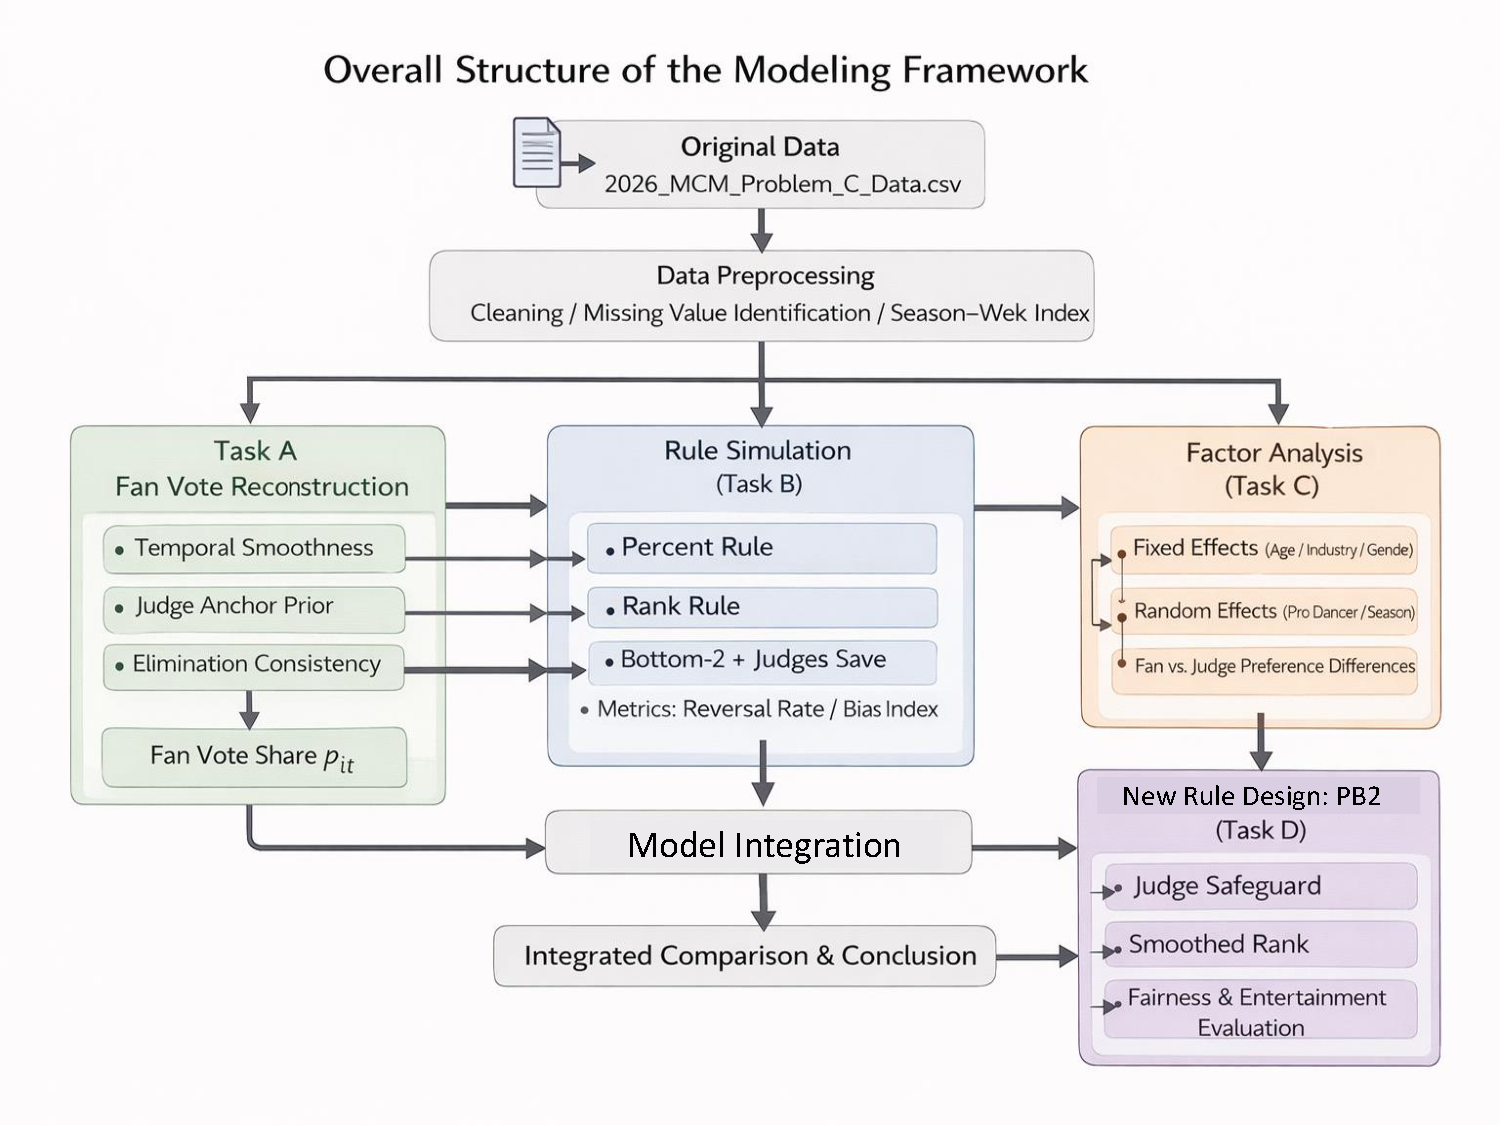
\includegraphics[width=0.65\linewidth]{output/fig/task3/overview.pdf}
  \caption{End-to-end workflow: infer latent fan support from observed eliminations, then use it to evaluate and redesign voting rules.}
  \label{fig:workflow_overview}
\end{figure}

\textbf{We model DWTS as a replayable inverse problem: infer latent fan support from observed eliminations, then use it to evaluate and redesign voting rules.}
(An end-to-end workflow summary is provided in the Summary Sheet; we keep the Introduction focused on motivation and contributions.)

\textbf{Our contributions are as follows.}
\begin{itemize}
  \item \textbf{Replay-ready data representation.}
  We build a canonical season-week-contestant panel with an explicit \texttt{active} set to ensure that all denominators and eligibility conditions match the show's mechanics (and that post-exit padding records do not contaminate comparisons).

  \item \textbf{Latent vote-share inference with uncertainty.}
  We infer weekly fan vote \emph{shares} by solving a constrained optimization problem whose feasibility encodes elimination consistency; slack handles exceptional weeks, and a smoothness prior selects stable explanations.
  The output includes both point estimates and uncertainty summaries (feasible ranges / sensitivity margins), supporting identifiability-aware interpretation.

  \item \textbf{Counterfactual rule evaluation via replay.}
  Using the inferred fan support, we replay eliminations under alternative aggregation schemes (rank vs.\ percent) and the incumbent Bottom-2 + judges' save mechanism, and quantify outcome divergence and robustness with replay-based metrics aligned to the show's decisions.

  \item \textbf{Mechanism analysis and transparent redesign (Task D2).}
  We fit interpretable statistical models to separate drivers of judges' scoring from fan preference (e.g., professional-dancer and celebrity-attribute effects), and propose \textit{Professional Bottom-2} (PB2): judges define the Bottom-2 risk set, while fan influence is applied only within that gate via a transparent blended score.
  PB2 is validated by replay-based stress tests (stability, controversial-case replays, and a unified bias test).
\end{itemize}

The remainder of the paper is organized as follows:
Section~2 formalizes tasks, assumptions, and notation;
Section~3 describes data processing and feature construction;
Sections~4--7 present vote inference, rule replay, mechanism analysis, and PB2 with robustness tests;
Section~8 concludes; and Section~9 provides a memo to management.


\section{Problem Decomposition and Analysis}\label{sec:problem_decomposition_and_analysis}
\textbf{This section formalizes DWTS as a replayable inverse problem and specifies the modeling objects that close our pipeline.}
We define the weekly active set, the observable judges' score signal, and the realized elimination outcomes, then introduce the latent fan vote share $p_{i,t}$ as the primary unknown.
Our inference module outputs point estimates $\hat p_{i,t}$ together with uncertainty summaries, which feed a unified rule replay engine; this engine generates counterfactual elimination paths used for rule comparison, case-based attribution, and the validation of a proposed new voting system.

% ===========================问题分解与分析=============================
\subsection{Problem Decomposition}\label{sec:problem_decomposition}

\textbf{We decompose the prompt into four linked tasks with shared inputs and a common replay-based evaluation layer.}
\begin{itemize}
    \item \textbf{Task A: Fan vote inference with uncertainty.}
    \textbf{Input:} weekly judges' scores and the realized eliminated set;
    \textbf{Output:} weekly fan vote shares $p_{i,t}$ (and uncertainty bands) over the active set;
    \textbf{Validation:} elimination-consistency under the assumed rule, plus identifiability diagnostics (feasible-range widths and margin-based sensitivity).

    \item \textbf{Task B: Voting-rule comparison via replay.}
    \textbf{Input:} judges' scores and inferred $p_{i,t}$;
    \textbf{Output:} counterfactual week-by-week eliminations under percent-based vs.\ rank-based aggregation (and variants);
    \textbf{Validation:} season-level and week-level outcome divergence measures and ``fan bias'' indicators.

    \item \textbf{Task C: Controversial contestants and judges' save attribution.}
    \textbf{Input:} inferred $p_{i,t}$ and replay engine;
    \textbf{Output:} case-study narratives supported by counterfactual trajectories with/without bottom-two judges' save;
    \textbf{Validation:} whether the mechanism explains observed controversies and how sensitive conclusions are to vote uncertainty.

    \item \textbf{Task D: Mechanism analysis and new system design.}
    \textbf{Input:} panel features (celebrity attributes, professional dancer identifiers) and inferred votes;
    \textbf{Output:} mixed-effects estimates for drivers of judges' scoring versus fan preference, and a parameterized voting rule;
    \textbf{Validation:} historical replay, robustness checks, and sensitivity analysis over hyperparameters and rule-switch assumptions.
\end{itemize}


% ==========================关键假设=============================
\subsection{Key Assumptions}\label{subsec:assumptions}

We adopt a small, testable assumption budget to make the inverse problem well-posed while keeping conclusions falsifiable.
\begin{enumerate}
    \item \textbf{Share normalization.} Fan votes are modeled as within-week shares over the active set.
    \item \textbf{Rule-governed elimination.} Eliminations follow the documented aggregation rule (percent-based or rank-based), optionally augmented by bottom-two judges' save where applicable.
    \item \textbf{Active-set definition and special episodes.} Post-exit ``zeros'' represent inactivity and are excluded from the active set; special episodes are explicitly flagged and may be accommodated via slack rather than forced exact compliance. When a counterfactual replay keeps an observed-exit contestant active, the required post-exit inputs are filled using a conservative, minimal-information imputation; this is used only to extend counterfactual trajectories and is not intended as a performance forecast.
    \item \textbf{Judges as observed signal.} Judges' scores provide an observed performance signal taken as exogenous to the voting mechanism.
    \item \textbf{Temporal smoothness.} Fan preference evolves smoothly week-to-week, motivating temporal regularization.
\end{enumerate}
The season at which the show returns to rank-based aggregation is treated as an explicit assumption and is stress-tested using adjacent cutoffs.

% =========================记号=============================
\subsection{Key Notations}\label{subsec:notations}
Table~\ref{tab:notations} summarizes indices, sets, observed quantities, latent fan vote shares, and rule-dependent combined scores used throughout the inference and replay pipeline.
\begin{table}[H]
\centering
\small
\begin{tabular}{ll}
\toprule
Symbol & Definition \\
\midrule
$s$ & Season index, $s=1,\dots,34$ \\
$t$ & Week index within season $s$ \\
$i$ & Contestant (celebrity--pro pair) index \\
$A_{s,t}$ & Active contestants in season $s$, week $t$ \\
$E_{s,t}$ & Eliminated set at end of week $t$; $m_{s,t}=|E_{s,t}|$ \\
$j_{i,t,k}$ & Score given by judge $k$ to contestant $i$ in week $t$ \\
$J_{i,t}$ & Total judges' score: $J_{i,t}=\sum_{k} j_{i,t,k}$ (skip missing) \\
$q^{J}_{i,t}$ & Judges' share: $q^{J}_{i,t}=J_{i,t}\big/\sum_{r\in A_{s,t}}J_{r,t}$ \\
$p_{i,t}$ & Fan vote share (latent), $\sum_{i\in A_{s,t}}p_{i,t}=1$ \\
$\alpha$ & Weight on judges under percent rule (default $\alpha=0.5$; stress-tested) \\
$S^{(P)}_{i,t}$ & Percent combined score: $S^{(P)}_{i,t}=\alpha q^{J}_{i,t}+(1-\alpha)p_{i,t}$ \\
$R^{J}_{i,t},R^{V}_{i,t}$ & Judges rank and fan rank (descending) \\
$R^{(R)}_{i,t}$ & Rank combined score: $R^{(R)}_{i,t}=R^{J}_{i,t}+R^{V}_{i,t}$ \\
$\xi_t$ & Slack for elimination-consistency; penalized in vote inference \\
$\lambda$ & Penalty weight on slacks in vote inference objective \\
\bottomrule
\end{tabular}
\caption{Core notations used throughout the paper.}
\label{tab:notations}
\end{table}

\subsection{Tasks and Evaluation KPIs}\label{subsec:tasks_and_kpis}

Our workflow consists of four tightly coupled tasks. \textbf{Task A} reconstructs latent weekly fan vote shares $p_{i,t}$
for each active contestant by solving a season-level constrained optimization problem that enforces elimination consistency
(with slack) under the documented mechanics\cite{bubeck2015convex,boyd2004convex}. \textbf{Tasks B/C} use these inferred votes to replay each season under
alternative aggregation rules (rank-based vs.\ percent-based, optionally with a bottom-two judges' save), producing
counterfactual eliminations and placements. \textbf{Task D1} fits mixed-effects models to contrast the drivers of judges'
evaluations versus audience support (celebrity attributes and professional partners). \textbf{Task D2} proposes an
implementable voting rule and selects parameters via replay-based stress tests.

To evaluate models and rule variants consistently, we use the following KPIs and slices.

\textbf{KPI1: Elimination Set Agreement (Jaccard Similarity).}
On each season-week $(s,t)$, we compute the replayed eliminated set $\hat{E}_{s,t}$ under a specified rule
and compare it to the observed eliminated-at-end-of-week set $E_{s,t}$ parsed from results. We measure
set-level agreement by the Jaccard similarity
\[
J_{s,t}=\frac{|E_{s,t}\cap \hat{E}_{s,t}|}{|E_{s,t}\cup \hat{E}_{s,t}|}.
\]
KPI1 is reported as the week-level mean of $J_{s,t}$ over all counted season-week instances.
Weeks with no elimination yield $E_{s,t}=\varnothing$ (and possibly $\hat{E}_{s,t}=\varnothing$); we adopt the
convention $J_{s,t}=1$ when both sets are empty and include such weeks in the mean.

\paragraph{KPI3: Rule Divergence Rate (Rank vs.\ Percent).}
Holding the same vote input (e.g., BL-0 proxy or inferred votes), KPI3 measures how often two aggregation schemes disagree
on eliminations:
\begin{equation}
\text{KPI3}=\frac{\sum_{(s,t)\in\Omega}\mathbf{1}\{\widehat{E}^{\text{rank}}_{s,t}\neq \widehat{E}^{\text{percent}}_{s,t}\}}{|\Omega|},
\end{equation}
where $\Omega$ denotes eligible $(s,t)$. KPI3 is reported descriptively as ``impact magnitude,'' not as an optimization objective.

\paragraph{KPI2: Vote Identifiability (interval tightness).}
Because votes are unobserved, vote inference is not always identifiable.\cite{benning2018regularization,kaipio2005statistical} For each $(s,t,i)$, we compute a feasible interval
$[p^{\min}_{i,t},p^{\max}_{i,t}]$ over fan vote shares consistent with elimination constraints (and with a near-optimal shell
around the Task~A objective). We define an identifiability score as
\begin{equation}
ID_{i,t}=\frac{1}{p^{\max}_{i,t}-p^{\min}_{i,t}+\varepsilon},
\end{equation}
and summarize by quantiles across contestants, weeks, and seasons. KPI2 flags weeks and contestants where multiple vote
allocations explain the observed elimination equally well.

\paragraph{Reproducible baseline (BL-0).}
Before introducing inferred votes, we report KPI1/KPI3 under BL-0 as an audit baseline. In BL-0, the rank scheme reduces to
judges' ranks only (uniform fan ranks add a constant), and the percent scheme uses judges' percent plus a uniform fan share
$1/n_{\text{active}}$. BL-0 validates denominator handling and replay mechanics, but it is not used to claim audience preference estimates.



\section{Data Processing and Analysis}\label{sec:data}
% =========================
% Section 3: Data Processing and EDA (model-driven)
% =========================


\subsection{Data Cleaning Principles and Validation}
\label{subsec:cleaning_principles_validation}

\subsubsection{Cleaning Principles}
\label{subsubsec:cleaning_principles}

Our preprocessing is \emph{model-driven}: we only perform transformations required to
(i) construct a reproducible season--week--contestant panel,
(ii) define eligibility/denominator rules for KPI computation, and
(iii) enable counterfactual replay under alternative voting schemes.
We preserve the dataset's official encodings and remove their influence through an explicit
\emph{active-set} definition rather than aggressive imputation \cite{comap2026_problemC_pdf}.

\paragraph{Principle A --- Respect official encodings (0 scores, N/A, irregular season length).}
The official problem statement clarifies that (i) weeks with no elimination or multiple eliminations exist,
(ii) \texttt{N/A} can mean either ``no 4th judge'' or ``weeks beyond a season's actual run'',
and (iii) a score of 0 is recorded for celebrities after elimination (post-exit padding).
We therefore treat these as \emph{structural encodings} rather than noise \cite{comap2026_problemC_pdf}.

\paragraph{Principle B --- Eligibility controls denominators (active-set construction).}
A contestant is considered active in $(s,t)$ if at least one judge score exists for that week and the week
does not exceed the contestant's exit week (eliminated week parsed from \texttt{results}, or an inferred
withdraw week). Post-elimination zeros are retained for auditability but excluded from denominators via
\texttt{active=\textbf{false}}.

\paragraph{Principle C --- Within-week aggregation only; no judge identity tracking.}
Because judge indices are not persistent identities across weeks/seasons, we only use within-week aggregates
(weekly total, rank, and percent) and avoid modeling judge-specific time series at the preprocessing stage
\cite{comap2026_problemC_pdf}.

\paragraph{Principle D --- Non-single-elimination weeks are handled explicitly.}
Weeks with zero eliminations are excluded from the single-elimination consistency denominator, while
multi-elimination weeks are evaluated via bottom-$k$ set matching (set-match).


\subsubsection{Data Cleaning Operations}
\label{subsubsec:cleaning_operations}

We implement a deterministic pipeline that reshapes the original wide-format judge-score columns into a long
panel and then attaches minimal labels required for downstream inference and replay:

\begin{enumerate}
  \item \textbf{Wide-to-long reshaping.}
  We reshape \texttt{weekX\_judgeY\_score} into one row per $(season, week, celebrity)$, and compute
  \texttt{all\_judges\_nan} and
  \texttt{total\_judge\_score = sum(judge\_scores, skipna=\{True\})}
  to respect varying judge counts.

  \item \textbf{Exit mapping and labels.}
  We parse elimination week from \texttt{results} when available; otherwise, for withdrew/finished cases we infer
  \texttt{exit\_week} as the last week with a positive total score, falling back to the last non-missing scored week.
  We store \texttt{exit\_type} $\in \{\text{withdrew}, \text{eliminated}, \text{finished}\}$ and define
  \texttt{true\_elim\_flag} only for elimination exits by default.

  \item \textbf{Active-set definition and anomaly flag.}
  We define \texttt{active = (not all\_judges\_nan) \& (week $\le$ exit\_week)}.
  Additionally, if \texttt{total\_judge\_score == 0} occurs outside the inferred exit week, we flag
  \texttt{data\_anomaly\_zero\_score=1} and force \texttt{active=false} to prevent padded zeros from contaminating denominators.

  \item \textbf{Within-week relative measures.}
  For each $(season, week)$, among active contestants only, we compute \texttt{judge\_rank} (1 = best) and
  \texttt{judge\_percent = score / sum(scores)} when the denominator is positive.
\end{enumerate}


\subsubsection{Data Cleaning Outcomes and Validation}
\label{subsubsec:cleaning_outcomes_validation}

\paragraph{Outcomes (artifacts and interfaces).}
The output of preprocessing is a \emph{canonical weekly panel}
(\texttt{output/table/intermediate\_weekly\_panel.csv}) that contains eligibility/exit labels
(\texttt{active}, \texttt{exit\_type}, \texttt{exit\_week}, \texttt{true\_elim\_flag}) and judge-based within-week features
(\texttt{total\_judge\_score}, \texttt{judge\_rank}, \texttt{judge\_percent}).
This panel is the single input interface used for all downstream KPI recomputation, vote-share inference, and replay simulation.

In addition, we generate audit/debug artifacts: (i) a week-level prediction table
(\texttt{output/table/intermediate\_baseline\_preds.csv}) and (ii) a report-ready \LaTeX{} table
(\texttt{output/table/tab\_baseline\_consistency.tex}) plus an optional figure
(\texttt{output/figure/fig\_fliprate\_by\_season.pdf}).

\paragraph{Validation (what we check, and why it is sufficient for P0).}
We validate preprocessing through three audit layers:
\begin{itemize}
  \item \textbf{(V1) Encoding-consistency checks.}
  We follow the official semantics for \texttt{N/A} and post-elimination zeros, preserving these encodings and excluding them
  from denominators via \texttt{active} \cite{comap2026_problemC_pdf}.

  \item \textbf{(V2) Denominator/eligibility invariants.}
  \texttt{judge\_percent} is computed only among active contestants within each $(season, week)$; when total score is positive,
  it sums to one within the active set. The explicit \texttt{data\_anomaly\_zero\_score} flag prevents accidental inclusion of padded zeros.

  \item \textbf{(V3) End-to-end reproducibility via BL-0 sanity check.}
  On top of the canonical panel, we implement the BL-0 baseline (rank: judge-rank only; percent: judge-percent plus uniform
  $1/n_{\text{active}}$) and reproduce a consistent set of KPI1/KPI3 summaries across era slices.
  This serves as a pipeline sanity check rather than a final model claim.
\end{itemize}

\noindent\textbf{BL-0 sanity-check summary (reportable, not a final claim).}
Under BL-0, the overall elimination hit-rate is 0.364 (rank) and 0.375 (percent) across 264 eligible weeks,
and the rank-vs-percent flip rate is 0.038.


\subsection{Panel Construction}
\label{subsec:panel_construction}

Panel construction converts the wide-format score table into a long-format dataset where each record corresponds to a unique
$(season, week, celebrity)$ unit. We reshape \texttt{weekX\_judgeY\_score} into such a long panel and compute weekly aggregates
(\texttt{total\_judge\_score}) and within-week relative measures (\texttt{judge\_rank}, \texttt{judge\_percent}) among the active set.
We then attach deterministic exit/eligibility labels (\texttt{exit\_type}, \texttt{exit\_week}, \texttt{true\_elim\_flag}, \texttt{active})
derived from \texttt{results} and score availability. This panel is the canonical input shared by all subsequent modules, including
vote-share inference and counterfactual replay under alternative voting schemes.


\subsection{Empirical Findings from EDA (only what feeds models)}
\label{subsec:eda_model_driven}

\subsubsection{Data Visualization}
\label{subsubsec:eda_viz}

We summarize baseline consistency and rule divergence using:
\begin{itemize}
  \item \textbf{(L1 table)} \texttt{output/table/tab\_baseline\_consistency.tex}:
  BL-0 elimination hit-rate under rank and percent schemes (KPI1) and rule divergence (KPI3/FlipRate), with slices:
  Overall / Rank-era / Percent-era.
  \item \textbf{(L2 figure, optional)} \texttt{output/figure/fig\_fliprate\_by\_season.pdf}:
  season-level visualization of where the two schemes disagree.
\end{itemize}

% If you want to include the table/figure directly:
% \begin{table}[t]
%   \centering
%   \begin{tabular}{lrrrr}
\hline
Slice & $N_{\mathrm{weeks}}$ & Hit-Rate (Rank) & Hit-Rate (Percent) & FlipRate \\
\hline
Overall & 264 & 0.364 & 0.375 & 0.038 \\
Rank-era (S1-2,28-34) & 66 & 0.348 & 0.364 & 0.015 \\
Percent-era (S3-27) & 198 & 0.369 & 0.379 & 0.045 \\
\hline
\end{tabular}
%   \caption{BL-0 baseline consistency and rule divergence across era slices.}
%   \label{tab:baseline_consistency}
% \end{table}
%
% \begin{figure}[t]
%   \centering
%   
\includegraphics[width=\linewidth]{output/figure/fig_fliprate_by_season.pdf}
%   \caption{Season-level flip rate between rank- and percent-based BL-0 predictions.}
%   \label{fig:fliprate_by_season}
% \end{figure}


\subsubsection{Key Empirical Findings}
\label{subsubsec:key_findings}

\paragraph{Finding 1 --- A reproducible BL-0 baseline exists and is non-trivial.}
Using only judge-based information and a uniform fan proxy, BL-0 yields measurable elimination-consistency hit-rates under both
rank and percent aggregation, and a non-zero flip rate between the two schemes. These quantities are used strictly as a sanity check
for the pipeline and as a reference point for later vote-inference models.

\paragraph{Finding 2 --- Rule comparisons must be stress-tested around the season-28 cutoff.}
We adopt the era split for rule-comparison slicing (Rank-era vs. Percent-era), but treat the season-28 switch as an assumption and
stress-test adjacent cutoffs.

\paragraph{Finding 3 --- Non-standard weeks materially affect denominators.}
Because the dataset includes weeks with no elimination or multiple eliminations, KPI denominators must explicitly exclude no-elimination
weeks and handle multi-elimination weeks via set matching; otherwise consistency metrics can be inflated.


\subsection{Feature Engineering}
\label{subsec:feature_engineering}

We keep feature engineering minimal and aligned with downstream modeling needs:

\begin{itemize}
  \item \textbf{Performance signals (week-level, within active set).}
  \texttt{total\_judge\_score}, \texttt{judge\_rank}, and \texttt{judge\_percent} are computed per $(season, week)$ among active contestants
  and serve as the observed performance component when replaying elimination rules or inferring latent vote shares.

  \item \textbf{Explanatory covariates (contestant-level, for heterogeneity analysis).}
  When available, we use \texttt{ballroom\_partner} (pro dancer identity), \texttt{celebrity\_age\_during\_season},
  \texttt{celebrity\_industry}, and region-related fields for slicing and mixed-effects heterogeneity analyses.
\end{itemize}


\subsection{Synthesis of Findings}
\label{subsec:synthesis_findings}

In summary, our preprocessing produces a canonical season--week--contestant panel that
(i) respects the official encodings of \texttt{N/A} and post-elimination zeros,
(ii) enforces denominator correctness through an explicit active-set definition, and
(iii) enables reproducible baseline replay consistent with our KPI definitions.
Key data caveats---non-standard elimination weeks, varying judge availability, and the uncertain season-28 era cutoff---are surfaced
explicitly for robustness stress tests rather than hidden by aggressive cleaning \cite{comap2026_problemC_pdf}.


\section{Task A: Fan Vote Inference Model}\label{sec:A}
We propose a deployable, data-driven fan vote inference model. The key design principle is to \textbf{treat audience votes as a latent signal and infer vote shares from observed judges' scores and elimination outcomes under explicit rule constraints.}

\subsection{Overview and Modeling Philosophy}\label{subsec:model_philosophy}

\textbf{Fan votes are a latent signal and must be inferred indirectly.}
In DWTS, eliminations depend on a combination of judges' scores and audience votes, yet only judges' scores and realized eliminations are observed.
We therefore model weekly audience support as a latent vote-share vector over the active set.
Because many vote configurations can be consistent with the same elimination outcome, the inference problem is generally underdetermined; our approach resolves this by
(i) enforcing elimination-consistency constraints implied by the show's rule mechanics and
(ii) selecting a stable solution via temporal smoothness regularization.\cite{benning2018regularization,kaipio2005statistical}
Special episodes (e.g., no-elimination or irregular-format weeks) are handled explicitly through slack variables rather than forcing exact compliance, and these slacks become a diagnostic for identifiability and model mismatch.

\subsection{Main Inference Model}\label{subsec:inference_model}
\textbf{Decision variables.}
For each season $s$, week $t$, and active contestant $i\in A_{s,t}$, let $p_{i,t}\ge 0$ denote the unobserved fan vote share, with $\sum_{i\in A_{s,t}}p_{i,t}=1$.
Let $J_{i,t}$ be the observed total judges' score (sum across judges with missing values skipped) and define the judges' share
$q^J_{i,t}=J_{i,t}\big/\sum_{r\in A_{s,t}}J_{r,t}$.

\textbf{Percent-scheme combined score (primary inference target).}
Under the percent-based aggregation, we define the combined score
\begin{equation}
S^{(P)}_{i,t}=\alpha q^{J}_{i,t}+(1-\alpha)p_{i,t},
\end{equation}
where $\alpha\in[0,1]$ controls the relative weight of judges versus fans (default $\alpha=0.5$; later stress-tested).

\textbf{Elimination-consistency constraints with slack.}
Let $E_{s,t}\subseteq A_{s,t}$ denote the observed eliminated set at the end of week $t$ with $m_{s,t}=|E_{s,t}|$.
We introduce a nonnegative slack $\xi_t\ge 0$ and impose
\begin{equation}
S^{(P)}_{e,t}\le S^{(P)}_{i,t}+\xi_t,\quad \forall e\in E_{s,t},\ \forall i\in A_{s,t}\setminus E_{s,t}.
\end{equation}

When the assumed rule and data are perfectly compatible, the minimum feasible $\xi_t$ is zero; otherwise $\xi_t>0$ quantifies the smallest violation needed to reconcile the observed outcome.\cite{aitchison1986compositional}
\paragraph{Objective with judge-anchor prior.}
To avoid degenerate ``nearly-uniform'' vote reconstructions, we add a judge-anchor prior that pulls fan vote shares toward
judges' score shares in the absence of strong contradictory evidence. For each season $s$, we solve:
\begin{align}
\min_{\{p_{i,t}\},\{\xi_t\}} \quad
& \underbrace{\sum_{t=2}^{T_s}\sum_{i\in A_{s,t}\cap A_{s,t-1}}(p_{i,t}-p_{i,t-1})^2}_{\text{Temporal smoothness}}
+ \lambda_1 \underbrace{\sum_{t=1}^{T_s}\sum_{i\in A_{s,t}}(p_{i,t}-q^J_{i,t})^2}_{\text{Judge anchor prior}}
+ \lambda_2 \underbrace{\sum_{t=1}^{T_s}\xi_t^2}_{\text{Violation penalty}} \label{eq:taskA_obj_anchor}\\
\text{s.t.}\quad
& \sum_{i\in A_{s,t}} p_{i,t}=1,\ \ p_{i,t}\ge 0,\ \ \xi_t\ge 0, \qquad \forall t, \nonumber\\
& S^{(P)}_{e,t} \le S^{(P)}_{k,t} + \xi_t,\quad \forall t,\ \forall e\in E_{s,t},\ \forall k\in A_{s,t}\setminus E_{s,t}. \nonumber
\end{align}




\textbf{Remark (objective form).}
Equation~\eqref{eq:taskA_obj_anchor} is a convex quadratic program (QP) solved independently for each season.
The smoothness term is computed only for contestants active in consecutive weeks ($A_{s,t}\cap A_{s,t-1}$), while the anchor and slack penalties
apply to all active contestants and weeks. Hyperparameters $(\lambda_1,\lambda_2)$ are selected by replay-based diagnostics (Section~\ref{subsec:a_hyper_impl}).\cite{boyd2004convex,bubeck2015convex}

\begin{algorithm}[H]
\caption{Season-wise fan vote inference via constrained QP}
\label{alg:qp_inference}
\small  % 字号缩小，避免公式溢出
\begin{algorithmic}[1]  % [1] 表示显示行号，algpseudocode必须加
    % ---- 输入输出定义（algpseudocode标准写法）----
    \Require 
        Weekly panel for season $s$: active sets $A_{s,t}$, judges' totals $J_{i,t}$, eliminated sets $E_{s,t}$; hyperparameters $\alpha,\lambda_1,\lambda_2$.
    \Ensure 
        Point estimates $\hat p_{i,t}$ and slack diagnostics $\hat \xi_t$ for all eligible weeks.

    % ---- 算法步骤 ----
    \State Compute judges' share for each week $t$: 
    \[
    q^J_{i,t} = \frac{J_{i,t}}{\sum_{r\in A_{s,t}} J_{r,t}}
    \]
    \State Define decision variables $\{p_{i,t}\}_{i\in A_{s,t}}$ with constraints:
    \[
    p_{i,t} \ge 0, \quad \sum_{i\in A_{s,t}} p_{i,t} = 1
    \]
    \State For each week $t$, define percent-based composite score $S^{(P)}_{i,t}$ and slack variable $\xi_t$:
    \[
    S^{(P)}_{i,t} = \alpha q^{J}_{i,t} + (1-\alpha)p_{i,t}, \quad \xi_t \ge 0
    \]
    \State Add elimination-consistency constraints:
    \[
    S^{(P)}_{e,t} \le S^{(P)}_{i,t} + \xi_t \quad \forall e\in E_{s,t}, \, i\in A_{s,t}\setminus E_{s,t}
    \]
    \State Solve the quadratic program (QP) to minimize the objective function:
    \[
    \mathcal{L} = \sum_{t=2}^{T_s}\sum_{i\in A_{s,t}\cap A_{s,t-1}} (p_{i,t}-p_{i,t-1})^2 + \lambda_1\sum_{t=1}^{T_s}\sum_{i\in A_{s,t}}(p_{i,t}-q^J_{i,t})^2 + \lambda_2\sum_{t=1}^{T_s}\xi_t^2
    \]
    \State Output $\hat p_{i,t}$ (inferred vote shares) and $\hat \xi_t$ (slack diagnostics); flag weeks with large $\hat \xi_t$ as potential special-episode mismatches.
\end{algorithmic}
\end{algorithm}

\subsection{Uncertainty Quantification and Sensitivity Analysis}\label{subsec:uncertainty_qualification_and_sensitivity_analysis}
\textbf{Uncertainty is intrinsic because the inverse problem is not fully identifiable.}
We report three complementary uncertainty summaries:
(i) \textbf{Feasible intervals:} for each $(i,t)$, compute the minimum and maximum $p_{i,t}$ attainable under the same constraints (yielding an interval width as an identifiability proxy, KPI2);
(ii) \textbf{Elimination margin:} quantify how much perturbation to $\hat p_{i,t}$ is required to flip the predicted eliminated set under the replay engine, providing a week-level stability score; and
(iii) \textbf{Slack diagnostics:} $\xi_t$ indicates weeks where observed outcomes cannot be matched under the assumed mechanics without violation; these weeks are flagged for special-episode handling and for sensitivity analysis over the rule-switch season and $\alpha,\lambda_1,\lambda_2$.


\subsubsection{KPI2: Vote Identifiability (interval tightness)}\label{subsubsec:kpi2_identifiability}

\textbf{KPI2: Vote Identifiability (interval tightness).}
The KPI registry defines vote identifiability by the tightness of a feasible interval for each $(s,t,i)$ under an explicit elimination mechanism.
In Task~A, we instantiate KPI2 under the \textbf{percent-based rule} with the fan vote \textbf{share} variable $p_{i,t}$, and set $\varepsilon=10^{-6}$ to avoid singularities.
After solving the season-wise inference QP and obtaining $(\hat p,\hat\xi)$ with optimal objective value $\mathrm{OPT}_s$, we compute a \textbf{near-optimal feasible interval} for each active contestant-week pair by solving two auxiliary profile problems:
\[
p^{\min}_{i,t}=\min p_{i,t},\qquad p^{\max}_{i,t}=\max p_{i,t},
\]
subject to the original probability and elimination-consistency constraints, plus a tolerance shell that keeps solutions comparable to the fitted trajectory:
\[
\mathcal{L}(p,\xi)\le (1+\delta_{\mathrm{obj}})\mathrm{OPT}_s,\qquad \xi_\tau \le \hat\xi_\tau+\delta_\xi \ \ (\forall \tau),
\]
where $\mathcal{L}(p,\xi)$ is the Task-A objective (smoothness + judge-anchor + slack penalty).
The interval width $w_{i,t}=p^{\max}_{i,t}-p^{\min}_{i,t}$ is mapped to an identifiability score
\[
\mathrm{ID}_{i,t}=\frac{1}{w_{i,t}+\varepsilon}.
\]
We summarize $\mathrm{ID}_{i,t}$ by median/quantiles across contestants and weeks and aggregate by season and by early/mid/late phases; in implementation we compute KPI2 on selected slices (e.g., late-phase weeks or controversial cases) to control computational cost.

\paragraph{Profile optimization formulation.}
\label{para:kpi2_profile_formulation}

For a fixed season $s$, let $T_s$ be the number of weeks.
Define decision variables
\[
\mathbf{p}=\{p_{j,\tau}: j\in A_{s,\tau},\ \tau=1,\dots,T_s\},\qquad
\boldsymbol{\xi}=\{\xi_\tau:\tau=1,\dots,T_s\}.
\]
For each week $\tau$, the percent-rule combined score is
\[
S^{(P)}_{j,\tau}=\alpha q^J_{j,\tau}+(1-\alpha)p_{j,\tau}.
\]

\textbf{Base constraints.}
We impose simplex constraints for each week:\cite{aitchison1986compositional,pawlowsky2015compositional,filzmoser2018compositional}
\begin{align}
& p_{j,\tau}\ge 0,\quad \forall j\in A_{s,\tau}, \forall \tau, \label{eq:kpi2_nonneg}\\
& \sum_{j\in A_{s,\tau}}p_{j,\tau}=1,\quad \forall \tau. \label{eq:kpi2_simplex}
\end{align}
Slacks are nonnegative:
\begin{equation}
\xi_\tau\ge 0,\qquad \forall \tau. \label{eq:kpi2_slack_nonneg}
\end{equation}
Elimination-consistency constraints (same as Task~A) are
\begin{equation}
S^{(P)}_{e,\tau}\le S^{(P)}_{k,\tau}+\xi_\tau,\quad \forall \tau,\ \forall e\in E_{s,\tau},\ \forall k\in A_{s,\tau}\setminus E_{s,\tau}.
\label{eq:kpi2_elim}
\end{equation}

\textbf{Near-optimal shell (to prevent uninformative, overly wide intervals).}
Let the Task-A objective be
\begin{equation}
\mathcal{L}(\mathbf{p},\boldsymbol{\xi})
=
\sum_{\tau=2}^{T_s}\sum_{j\in A_{s,\tau}\cap A_{s,\tau-1}}(p_{j,\tau}-p_{j,\tau-1})^2
+\lambda_1\sum_{\tau=1}^{T_s}\sum_{j\in A_{s,\tau}}(p_{j,\tau}-q^J_{j,\tau})^2
+\lambda_2\sum_{\tau=1}^{T_s}\xi_\tau^2.
\label{eq:kpi2_L_def}
\end{equation}
After solving the main inference QP, we obtain $(\hat{\mathbf{p}},\hat{\boldsymbol{\xi}})$ and $\mathrm{OPT}_s=\mathcal{L}(\hat{\mathbf{p}},\hat{\boldsymbol{\xi}})$.
To compute intervals around the fitted explanation, we add:
\begin{align}
& \mathcal{L}(\mathbf{p},\boldsymbol{\xi}) \le (1+\delta_{\mathrm{obj}})\,\mathrm{OPT}_s, \label{eq:kpi2_shell_quad}\\
& \xi_\tau \le \hat{\xi}_\tau+\delta_\xi,\qquad \forall \tau. \label{eq:kpi2_slack_cap}
\end{align}
In implementation, \eqref{eq:kpi2_shell_quad} can be written as a convex SOC constraint by noting that $\mathcal{L}$ is a sum of squares:
\[
\left\|
\begin{bmatrix}
\{p_{j,\tau}-p_{j,\tau-1}\}_{\tau=2..T_s,\ j\in A_{s,\tau}\cap A_{s,\tau-1}}\\[2pt]
\{\sqrt{\lambda_1}\,(p_{j,\tau}-q^J_{j,\tau})\}_{\tau=1..T_s,\ j\in A_{s,\tau}}\\[2pt]
\{\sqrt{\lambda_2}\,\xi_\tau\}_{\tau=1..T_s}
\end{bmatrix}
\right\|_2
\le
\sqrt{(1+\delta_{\mathrm{obj}})\,\mathrm{OPT}_s}.
\]
This SOC form is directly supported by standard convex solvers (e.g., via CVX frameworks).\cite{boyd2011admm}

\textbf{Profile-min and profile-max.}
For each active pair $(i,t)$ with $i\in A_{s,t}$, define:
\begin{align}
p^{\min}_{i,t} \;=\;& \min_{\mathbf{p},\boldsymbol{\xi}}\ \ p_{i,t} \label{eq:kpi2_profile_min}\\
\text{s.t.}\ \;& \eqref{eq:kpi2_nonneg}--\eqref{eq:kpi2_elim},\ \eqref{eq:kpi2_shell_quad}--\eqref{eq:kpi2_slack_cap}, \nonumber
\end{align}
and
\begin{align}
p^{\max}_{i,t} \;=\;& \max_{\mathbf{p},\boldsymbol{\xi}}\ \ p_{i,t} \label{eq:kpi2_profile_max}\\
\text{s.t.}\ \;& \eqref{eq:kpi2_nonneg}--\eqref{eq:kpi2_elim},\ \eqref{eq:kpi2_shell_quad}--\eqref{eq:kpi2_slack_cap}. \nonumber
\end{align}
We then set the interval width $w_{i,t}=p^{\max}_{i,t}-p^{\min}_{i,t}$ and identifiability score $\mathrm{ID}_{i,t}=1/(w_{i,t}+\varepsilon)$.

\begin{algorithm}[H]
\caption{KPI2 computation via profile optimization (per season)}
\label{alg:kpi2}
\small
\begin{algorithmic}[1]  % [1] 显示行号，algpseudocode 必须加
    % ---- 输入输出（algpseudocode 标准首字母大写）----
    \Require 
        Season $s$ weekly panel: active sets $A_{s,t}$, eliminated sets $E_{s,t}$, judges' shares $q^J_{i,t}$; 
        main-model hyperparameters $\alpha,\lambda_1,\lambda_2$; 
        KPI2 params $\varepsilon,\delta_{\mathrm{obj}},\delta_\xi$; 
        a slice selector $\mathcal{S}$ (set of $(i,t)$ pairs to evaluate).
    \Ensure 
        Interval bounds $\{p^{\min}_{i,t},p^{\max}_{i,t}\}$ and identifiability scores $\{\mathrm{ID}_{i,t}\}$ for $(i,t)\in\mathcal{S}$.

    % ---- 算法核心步骤 ----
    \State \textbf{Solve main inference QP} for season $s$ to obtain $(\hat{\mathbf{p}},\hat{\boldsymbol{\xi}})$ and $\mathrm{OPT}_s=\mathcal{L}(\hat{\mathbf{p}},\hat{\boldsymbol{\xi}})$.
    \State \textbf{Define common constraints}: simplex constraints \eqref{eq:kpi2_simplex}--\eqref{eq:kpi2_elim} and slack nonnegativity \eqref{eq:kpi2_slack_nonneg}.
    \State \textbf{Add KPI2 shells}: objective shell \eqref{eq:kpi2_shell_quad} (or its SOC form) and slack cap \eqref{eq:kpi2_slack_cap}.
    \State Choose evaluation slice $\mathcal{S}$ (e.g., late-phase weeks and/or controversial cases) to control computation.
    
    % 循环结构（algpseudocode 首字母大写）
    \For{each $(i,t)\in\mathcal{S}$}
        \State Solve profile-min optimization \eqref{eq:kpi2_profile_min} to get $p^{\min}_{i,t}$.
        \State Solve profile-max optimization \eqref{eq:kpi2_profile_max} to get $p^{\max}_{i,t}$.
        \State Compute width $w_{i,t}=p^{\max}_{i,t}-p^{\min}_{i,t}$ and identifiability score $\mathrm{ID}_{i,t}=1/(w_{i,t}+\varepsilon)$.
        \State Sanity check: verify $p^{\min}_{i,t}\le \hat p_{i,t}\le p^{\max}_{i,t}$; if violated, align constraints with the main QP.
    \EndFor
    
    \State Aggregate $\mathrm{ID}_{i,t}$ by week/season/phase using medians and quantiles as defined in the KPI registry.
\end{algorithmic}
\end{algorithm}

\subsection{Hyperparameters, tuning, and implementation details}
\label{subsec:a_hyper_impl}

\textbf{Hyperparameters and defaults.}
Task~A uses $\alpha$ (judge weight in the percent rule), $\lambda_1$ (strength of the judge-anchor prior),
$\lambda_2$ (penalty on constraint violations via $\xi_t$), and the KPI2 parameters $\varepsilon,\delta_{\mathrm{obj}},\delta_\xi$.
Unless otherwise stated, we set $\alpha=0.5$ as the nominal DWTS percent weighting and treat $\alpha$ as a sensitivity knob in later stress tests.

We tune $(\lambda_1,\lambda_2)$ by replay-based diagnostics. Increasing $\lambda_2$ enforces stricter elimination-consistency
(smaller $\xi_t$) at the cost of reduced feasibility for irregular-format weeks; decreasing $\lambda_2$ allows the model to absorb
format mismatches but may underfit eliminations. Increasing $\lambda_1$ pulls inferred votes toward judges' score shares and helps
avoid near-uniform solutions, while excessively large $\lambda_1$ may suppress genuine judge--fan disagreements that are evidenced by
the observed eliminations. Practically, we tune $(\lambda_1,\lambda_2)$ on a season-by-season basis by balancing
(i) the frequency and magnitude of nonzero slacks $\hat\xi_t$,
(ii) the stability of inferred top-$k$ vote shares across adjacent weeks, and
(iii) downstream replay fidelity in Task~B.

\textbf{Special episodes and multi-elimination weeks.}
Our formulation supports (a) multi-elimination weeks by allowing $|E_{s,t}|>1$ and enforcing the same pairwise inequalities against all non-eliminated contestants, and
(b) non-elimination or irregular weeks by allowing $E_{s,t}=\varnothing$ (no elimination constraints) while still solving the smoothness objective; such weeks can also be explicitly flagged and assessed via slack and sensitivity tests.
If a season contains weeks whose outcomes cannot be reconciled with the assumed mechanics, the model will surface this via persistently large $\hat\xi_t$; these weeks are treated as format exceptions rather than forcing ad hoc re-labeling.

\textbf{Solver and numerical stability.}
The main inference problem is a convex QP and can be solved season-wise using standard QP solvers.
The KPI2 shell can be implemented either directly as a quadratic constraint or in SOC form; the latter is solver-friendly in CVX frameworks.
To avoid numerical issues, we recommend
(i) normalizing judges' scores into shares $q^J$ (already done),
(ii) using $\varepsilon=10^{-6}$ for identifiability scoring,
and (iii) keeping $\delta_{\mathrm{obj}}$ small (e.g., 1--5\%) so profile intervals remain comparable to the fitted explanation.


\section{Task B \& C: Rule Reply, Volting System, and Counterfactuals}\label{sec:B_and_C}
% =========================
% Chapter 5: Rule Replay, Voting System, and Counterfactuals
% File: 5_rule_reply_volting_system_and_counterfactuials.tex
% =========================

% ---- Chapter opening positioning paragraph (results-focused, protocol explicit)
Following the official rule definitions, we perform season--week counterfactual replays under (i) rank-based aggregation and (ii) percent-based aggregation. We initialize each replay with the observed eligibility labels, but update the active set week-by-week according to the counterfactual eliminations under the chosen rule. When a counterfactual path keeps an observed-exit contestant active beyond the observed data horizon, we apply a conservative, minimal-information imputation solely to complete the replay (not to forecast future performance).
As a reproducible sanity-check baseline (BL-0), we use judge-only information with a uniform fan proxy
and report elimination hit-rate (KPI1) and the rule divergence rate (KPI3/FlipRate).
This chapter summarizes cross-season differences (Section~5.1), explains divergences via controversial case studies (Section~5.2),
evaluates the incremental impact of bottom-two and judges' save (Section~5.3), and synthesizes implications (Section~5.4).

\subsection{Rank vs. Percent Across Seasons}\label{subsec:rank_vs_percent_across_seasons}
Results in this section are first reported under BL-0 as a reproducible sanity check; Task A inferred votes are used in subsequent replays.
% 这里放：active set 口径、single-elim eligibility、special exits、tie-handling、以及“同一输入不同规则”的对比原则。
% 目标：评审只看这一段就不会质疑你们分母与口径。
  
% ---------------- FIG 5.1: FlipRate by season (eligible weeks only) ----------------
% 插入点 A：在 Cross-season summary metrics (KPI1 & KPI3) 第一段之后
% 用途：先给读者“全局敏感度”直观印象
% Fig 5.1 fig_fliprate_by_season.pdf（FlipRate by season，eligible only）
% -------------------------------------------------------------------------------
% Insert here to support KPI3/FlipRate cross-season comparison.
\begin{figure}[H]
    \centering
    \includegraphics[width=0.95\linewidth]{output/fig/fig5\_1\_fliprate\_by\_season.png}
    \caption{FlipRate by season under comparable (eligible) weeks.}
    \label{fig:fliprate_by_season}
\end{figure}
% -------------------------------------------------------------------------------

\subsubsection{Replay protocol and eligibility}\label{subsubsec:replay_protocol_and_eligibility}

\paragraph{Eligibility and special episodes.}
We treat eligibility as part of the replay interface: all week-level comparisons and KPI denominators are defined over the active set,
and special episodes (no-elimination weeks, multi-elimination weeks, withdrawals, and finals) are handled explicitly rather than being forced into a single-elimination template.
This design ensures that rule comparisons reflect the mechanics actually used on the show.

\paragraph{Aggregation rules (rank vs. percent).}
We replay eliminations under two official aggregation paradigms: rank-based and percent-based. For percent-based aggregation,
the combined score is
\[
S^{(P)}_{i,t}(\alpha)=\alpha q^{J}_{i,t}+(1-\alpha)\hat p_{i,t},
\]
and the replay eliminates the $m_{s,t}$ contestants with smallest $S^{(P)}_{i,t}(\alpha)$, where $m_{s,t}$ is the number of eliminations in week $(s,t)$.
For rank-based aggregation, we replace the score shares by within-week ranks and apply the same elimination logic.
Across both paradigms, ties are broken deterministically using a fixed secondary key (e.g., judges' score, then stable contestant ID), to preserve reproducibility.

\subsubsection{Cross-season summary metrics}\label{subsubsec:cross_season_summary_metrics}
We compute replay-based summary metrics over counted (season, week) instances under a unified eligibility convention.
KPI1 (Jaccard set agreement) summarizes week-level agreement between the observed eliminated set and the replayed eliminated set,
including no-elimination weeks via an explicit empty-set convention.
KPI3 (FlipRate) measures how often the predicted eliminated set differs between percent-based and rank-based replays under the same inputs.

\paragraph{Interpretation.}
We measure the bias to determine the degree of its inclination towards the audience, where a higher bias value indicates a greater tendency to favor the audience. 
According to Figure~\ref{fig:bias_index_comparison_four_methods_alpha0p5} we find that the \textit{percentage} method is more inclined towards the audience, yet the actual difference between the two methods is negligible compared with the \textit{PB2} we designed in \ref{subsubsec:d2_ruleB}.



\subsection{Controversial Contestants: Mechanism-driven Case Studies}\label{subsec:controversial_contestants_case_studies}

Aggregate metrics such as FlipRate identify \emph{where} rules diverge, but they do not explain \emph{why} a particular outcome
was perceived as controversial. We therefore adopt mechanism-driven case studies: each selected contestant represents a distinct
interaction between judges' performance signals and audience support under the incumbent ``combined Bottom-2 + judges' save'' pipeline
and under alternative aggregation semantics (rank vs.\ percent).

\paragraph{Selection rationale (what makes a case ``controversial'' in our framework).}
A contestant is considered controversial if their survival path is supported by a persistent mismatch between judges' signals and inferred fan support,
so that small changes in aggregation (rank vs.\ percent) or stage-ordering (when judges intervene) can plausibly alter the elimination boundary.
Operationally, we focus on seasons/episodes with elevated FlipRate and on contestants frequently cited in public discourse about judge--fan disagreement.
We analyze four representative contestants: Jerry Rice (Season~2), Billy Ray Cyrus (Season~4), Bristol Palin (Season~11), and Bobby Bones (Season~27).
All summaries are computed from \texttt{clean\_long\_data\_new1.csv} using \texttt{season}, \texttt{week}, \texttt{celebrity\_name}, \texttt{placement},
\texttt{elim\_week}, and judges-derived variables (\texttt{J\_total}, \texttt{J\_pct}, \texttt{active}).

\paragraph{Protocol (kept fixed across cases).}
For each contestant we report: (i) their within-season judges trajectory (e.g., week-level position under $q^J_{i,t}$), (ii) their inferred fan-support trajectory
through $\hat p_{i,t}$ (Task~A), and (iii) counterfactual replays under percent vs.\ rank aggregation with and without the judges' save module.
The objective is not to ``explain away'' controversy, but to isolate the minimal mechanism that makes the outcome boundary-sensitive.

\paragraph{Re-rank outcomes between \textit{percentage} and \textit{rank} rules for controversial contestants.} 
When we re-rank Jerry Rice under the \textit{percentage} rule and re-rank Billy Ray Cyrus, Bristol Palin and Bobby Bones under the \textit{rank} rule, 
we find that the final rankings of all four contestants drop significantly in the Tabel~\ref{tab:rank_percent}. This indicates a notable discrepancy in the tolerance for controversial 
contestants after the rule adjustment, and we will analyze these characteristics in the subsequent sections.

\begin{table}[htbp]
  \centering
  \caption{Rank and Percent Data Table} % 表格标题，可自行修改
  \begin{tabular}{lcccccc} % l=左对齐，c=居中对齐，7列对应7个字段
    \toprule
    name & season & canon & rank & percent & percent\_last\_two & bottom\_two \\
    \midrule
    Billy Ray Cyrus & 4 & 5 & 10 & 5 & 10 & 6 \\
    Bobby Bones    & 27 & 1 & 4 & 4 & 1 & 5 \\
    Bristol Palin  & 11 & 3 & 3 & 3 & 3 & 4 \\
    Bristol Palin  & 15 & 9 & 13 & 9 & 13 & 12 \\
    Jerry Rice     & 2 & 2 & 2 & 3 & 3 & 4 \\
    \bottomrule
  \end{tabular}
  \label{tab:rank_percent} % 表格交叉引用标签，可自行修改
\end{table}

\paragraph{Case 1: Jerry Rice (Season~2) --- early-era aggregation sensitivity.}
This case illustrates how early-season aggregation semantics can amplify judge--fan discordance: a contestant can remain viable when fan support offsets weak
judges' scores, yet the elimination boundary becomes sensitive to whether scores are combined as ranks or as normalized shares.
In our replay framework, small changes in aggregation can change which contestants enter the Bottom-2 risk set, which then cascades through subsequent weeks.

\paragraph{Case 2: Billy Ray Cyrus (Season~4) --- boundary effects without outcome reversal.}
Not every ``controversial'' public narrative implies a counterfactual outcome reversal. This case serves as a negative control: despite persistent discussion,
our replays indicate that the elimination week can remain stable under the incumbent pipeline.
We retain it to show that controversy perception can arise from judges--fan disagreement even when the realized elimination is not easily flipped by reasonable rule perturbations.

\paragraph{Case 3: Bristol Palin (Season~11) --- popularity protection under fan-sensitive boundaries.}
This case represents a common mechanism in celebrity competitions: strong fan support can keep a weak performer out of the Bottom-2 set for multiple weeks,
especially when the risk set is defined by a combined score.
When a judges' save is applied only after the Bottom-2 is formed, the mechanism protects technical merit only at the final step and cannot prevent fan support from shaping entry into the risk set.

\paragraph{Case 4: Bobby Bones (Season~27) --- late-era mismatch and institutional interpretation.}
This case highlights that the same observed trajectory can be interpreted differently depending on institutional design.
Under the incumbent ``combined Bottom-2 + judges' save'' pipeline, fan support can strongly affect who enters the risk set;
under a professionalism-first gate (Task~D2), the risk set is defined by judges alone, which changes whether fan support can ``rescue'' a weak performer.
We use this case to motivate why stage-ordering (gate vs.\ final save) is a central institutional lever rather than a cosmetic change.



\paragraph{Mechanisms synthesized across cases.}
Across the four examples we observe three recurring mechanisms:
(i) \textbf{aggregation semantics} (rank vs.\ percent) can shift the boundary of who is at risk;
(ii) \textbf{risk-set formation} is often more consequential than the final tie-break or save decision; and
(iii) \textbf{stage-ordering} determines whether judges' influence acts as a last-step safeguard (incumbent) or as a professionalism-first gate (Task~D2).
These mechanisms explain why controversies cluster around boundary-sensitive weeks and motivate the institutional redesign evaluated in Section~7.


\subsection{Bottom-two and Judges' Save Mechanism}\label{subsec:bottom_two_and_judges_save}

Some later seasons introduce a two-stage mechanism: (i) identify a bottom subset using the vote aggregation rule, then (ii) select the eliminated contestant from that subset via judges' save.
To isolate the incremental effect of this change, we implement a modular judges' save layer that can be toggled on top of either percent-based or rank-based aggregation.

\textbf{Module definition.} In a week with a bottom-two format, the replay first forms a bottom-two set $B_{s,t}$ using the chosen aggregation rule.
The saved contestant is the one with higher judges' score $J_{i,t}$ (equivalently higher $q^J_{i,t}$), and the other is eliminated.
This construction cleanly separates \emph{how the bottom set is formed} from \emph{how the final elimination is chosen}, enabling controlled counterfactual comparisons.

\textbf{Evaluation questions.} We quantify (a) how often the judges' save reverses the elimination implied by votes alone, (b) whether the save disproportionately protects contestants with strong judges' scores but weak fan support, and (c) how the mechanism affects overall rule divergence and late-season stability.
These results connect directly to management decisions about perceived fairness versus entertainment value.\cite{brandt2016comsoc,saari2001decisions}

\textbf{Illustrative case-study replay.} As a directional example, we run a Bottom-2 + judges' save replay with $\alpha=0.5$
(equal weight between $q^J_{i,t}$ and $\hat p_{i,t}$ in the combined score definition above) on Seasons~2/4/11/27.
Under this module, contestants whose survival historically relies on fan support tend to be eliminated earlier: Jerry Rice (S2) is eliminated in Week~7,
Bristol Palin (S11) in Week~9, and Bobby Bones (S27) in Week~8 in our replay, while Billy Ray Cyrus (S4) remains unchanged (Week~8).

\textbf{Caveat.} These outcomes can change for marginal weeks under different $\alpha$ values (we chose $\alpha \in [0.3, 0.7]$ in practice), tie-breaking conventions, and the semantics of
multi-elimination weeks (we apply eliminations sequentially when multiple eliminations occur), so we treat the above as illustrative rather than universal.




% ==========================规则概述与反事实分析=============================
\subsection{Synthesis of Findings from Rules}\label{subsec:synthesis_of_findings_from_rules}

We synthesize the rule replay evidence into actionable takeaways for both mechanism understanding and rule design.
First, rank versus percent aggregation differences are not uniformly distributed across seasons; they are amplified in weeks where contestants cluster near the elimination boundary, making the system sensitive to small score-share changes.
Second, the bottom-two + judges' save module acts as a structural preference for judges at the final decision margin, reducing the extent to which fan support can rescue a contestant once the contestant enters the bottom set.
Third, these rule interactions motivate the professionalism-first institutional redesign in Task D-2: moving the judges' influence from a final-step safeguard to a gating mechanism, while preserving watchability through structured late-stage suspense mechanisms evaluated via replay and stress testing.

% ---------------- OPTIONAL: Summary box (if you want a visual takeaway) ----------------
% Consider a small boxed summary here for Memo-ready bullets.
% -------------------------------------------------------------------------------




% =========================下面是我们粘图片的位置注释=================

% % ---------------- TAB 5.1: KPI1 hit-rate (rank vs percent) with era slices ----------------
% 用途：给出 KPI1（hit-rate）对照表，体现“fidelity vs sensitivity”
% Tab 5.1 tab_baseline_consistency.tex（Overall + era slices + #eligible weeks）
% -------------------------------------------------------------------------------
% % Insert here to report BL-0 sanity-check baseline consistency (eligible weeks only).
% \begin{table}[H]
%     \centering
%     %\begin{tabular}{lrrrr}
\hline
Slice & $N_{\mathrm{weeks}}$ & Hit-Rate (Rank) & Hit-Rate (Percent) & FlipRate \\
\hline
Overall & 264 & 0.364 & 0.375 & 0.038 \\
Rank-era (S1-2,28-34) & 66 & 0.348 & 0.364 & 0.015 \\
Percent-era (S3-27) & 198 & 0.369 & 0.379 & 0.045 \\
\hline
\end{tabular}
%     \caption{Elimination hit-rate (KPI1) for rank-based vs.\ percent-based replays (eligible weeks only), including era slices.}
%     \label{tab:kpi1_hitrate_era}
% \end{table}
% % -------------------------------------------------------------------------------

% % ---------------- FIG 5.2: Era cutoff stress test (27/28/29) ----------------
% 插入点 C：在 Era cutoff assumption and stress-test plan 段落之后
% 用途：一眼让评审看到“cutoff 变动对结论影响多大”，避免被质疑
% Fig 5.2 fig_cutoff_stress_test.pdf（cutoff=27/28/29 下的 FlipRate 或 hit-rate）
% -------------------------------------------------------------------------------
% % Insert here to show robustness of KPI1/KPI3 to era boundary assumption.
% \begin{figure}[H]
%     \centering
%     %\includegraphics[width=0.80\linewidth]{figures/fig_cutoff_stress_test.pdf}
%     \fbox{\parbox{0.80\linewidth}{\centering Placeholder: Fig 5.2 Era Cutoff Stress Test}}
%     \caption{Sensitivity of replay metrics to the assumed era cutoff (e.g., 27/28/29). Error bars denote bootstrap uncertainty over weeks.}
%     \label{fig:cutoff_stress_test}
% \end{figure}
% % -------------------------------------------------------------------------------

% % ---------------- FIG 5.3: FlipRate by season phase (early/mid/late) ----------------
% （P1 可选）插入点 D：如果你们写了“late-season 更敏感”的句子，就在那句之后插
% ---------------·------------------------------------------------
% % Only include if the text claims phase dependence (late-season sensitivity).
% \begin{figure}[H]
%     \centering
%     %\includegraphics[width=0.80\linewidth]{figures/fig_fliprate_by_phase.pdf}
%     \fbox{\parbox{0.80\linewidth}{\centering Placeholder: Fig 5.3 FlipRate by Phase}}
%     \caption{FlipRate by normalized season phase (eligible weeks only).}
%     \label{fig:fliprate_by_phase}
% \end{figure}
% % -------------------------------------------------------------------------------

% % ---------------- FIG 5.4x: Case timeline (judges vs fan) ----------------
% % 5.2 Controversial contestants case studies — 插图/表注释占位
% % 每个案例块建议插两张图（你们先留空位，等跑出来填）
% % 插入点 E：案例叙事中“Observed trajectory”之后
% % Fig 5.4a / 5.4b fig_case_<name>_timeline.pdf（judges rank、fan rank、淘汰标记）
% % -------------------------------------------------------------------------------
% % Insert inside each case study after "Observed trajectory".
% \begin{figure}[H]
%     \centering
%     %\includegraphics[width=0.90\linewidth]{figures/fig_case_JerryRice_timeline.pdf}
%     \fbox{\parbox{0.90\linewidth}{\centering Placeholder: Fig 5.4x Case Timeline}}
%     \caption{Case timeline example: week-by-week judges rank and inferred fan rank, with elimination markers.}
%     \label{fig:case_timeline_placeholder}
% \end{figure}
% % -------------------------------------------------------------------------------


% % ---------------- TAB 5.2x: Case counterfactual summary table ----------------
% % 插入点 F：在“Counterfactual replays”段落之后
% % Tab 5.2（小表） tab_case_<name>_counterfactual.tex：列出“真实淘汰 vs percent replay vs rank replay（含 save/不含 save）”
% % -------------------------------------------------------------------------------
% % Insert after "Counterfactual replays" to make the narrative audit-able.
% \begin{table}[H]
%     \centering
%     %\input{tables/tab_case_JerryRice_counterfactual.tex}
%     \caption{Case counterfactual summary: observed vs.\ percent vs.\ rank (and save variants if applicable).}
%     \label{tab:case_counterfactual_placeholder}
% \end{table}
% % -------------------------------------------------------------------------------


% % ---------------- FIG 5.5: Judges' save effect (elimination changed rate) ----------------
% % 5.3 Bottom-two and Judges' Save Mechanism — 插图注释占位
% % 插入点 G：在 “Evaluation questions” 段落之后
% % Fig 5.5 fig_save_fliprate.pdf：save 导致淘汰改变的比例（按 season 或按 week）
% % ------------------------------------------------------------------------------
% % Insert here to quantify how often judges' save changes the eliminated contestant.
% \begin{figure}[H]
%     \centering
%     %\includegraphics[width=0.85\linewidth]{figures/fig_save_fliprate.pdf}
%     \fbox{\parbox{0.85\linewidth}{\centering Placeholder: Fig 5.5 Judges' Save Effect}}
%     \caption{Impact of judges' save: rate at which the eliminated contestant changes relative to vote-only elimination.}
%     \label{fig:judges_save_effect}
% \end{figure}
% % -------------------------------------------------------------------------------


% % ------------------------FIG 5.6 fig_save_protection_profile.pdf------------------------
% （P1 可选）如果你们要支撑“save 更偏向保护技术高的人”：再加
% Fig 5.6 fig_save_protection_profile.pdf：被 save 的人通常 judges rank 更高但 fan rank 更低的比例（箱线/散点）
% ------------------------------------------------------------------------------

\section{Task D-1: Impact Analysis: Pro Dancers \& Celebrity Attributes}\label{sec:D1}
\subsection{Outcome definitions}
\label{subsec:outcome_definitions_d1}

To disentangle how outcomes are shaped by professional partners versus celebrity attributes, we model
judges' evaluations and inferred fan preferences as two distinct but related outcomes.
For comparability across seasons and weeks, we work with \emph{shares} rather than raw scores.
Let $A_{s,t}$ denote the active set in season $s$, week $t$.

\paragraph{Judges' outcome.}
Define the judges' score share
\begin{equation}
q^{J}_{i,t}=\frac{J_{i,t}}{\sum_{r\in A_{s,t}}J_{r,t}},
\end{equation}
and use a logit transform with a small $\epsilon$ for stability:
\begin{equation}
y^{J}_{i,t}=\log\frac{q^{J}_{i,t}+\epsilon}{1-q^{J}_{i,t}+\epsilon}.
\end{equation}

\paragraph{Fans' outcome.}
Let Task~A provide the inferred vote share $p_{i,t}$ (denoted $q^{V}_{i,t}$). We similarly define
\begin{equation}
y^{V}_{i,t}=\log\frac{p_{i,t}+\epsilon}{1-p_{i,t}+\epsilon}.
\end{equation}
We adopt share + logit for cross-season comparability and interpret coefficients on the log-odds scale.

\noindent\textbf{Elimination outcome.}
Define a weekly elimination indicator
\[
E_{i,t}=
\begin{cases}
1, & \text{if contestant $i$ is eliminated in week $t$,}\\
0, & \text{otherwise.}
\end{cases}
\]
This outcome links the two channels (judges' evaluations and inferred fan support) to realized competition survival.


\subsection{Modeling results: separating ``who judges reward'' vs.\ ``who fans support''}
\label{subsec:modeling_results_d1}

We fit two parallel mixed-effects models, one for judges and one for fans, with shared covariates but distinct
random-effects structures. This allows us to quantify whether professional dancers act primarily as
(i) performance amplifiers in the judges' channel, (ii) popularity amplifiers in the fans' channel, or both.

\subsubsection{Model 1: Judges' evaluation model}
\label{subsubsec:model1_judges}

We model judges' logit-share as
\begin{equation}
y^{J}_{i,t}=\beta_0 + X_i^\top\beta + f(t) + \mathrm{FE}_s + v_{d(i)} + u_{i} + \varepsilon^{J}_{i,t},
\end{equation}
where $X_i$ are celebrity attributes (e.g., age, industry), $f(t)$ captures week effects,
$\mathrm{FE}_s$ are season fixed effects, $v_{d(i)}$ is a random intercept for the professional dancer partnered with celebrity $i$,
and $u_i$ is a contestant random effect capturing persistent idiosyncrasy.
The variance component $\sigma_v^2$ represents the professional-dancer effect on judges' evaluations.

\paragraph{Hypothesis test.}
A key hypothesis test is $H_0:\sigma_v^2=0$ (no pro-dancer effect on judges).

\subsubsection{Model 2: Fans' preference model}
\label{subsubsec:model2_fans}

We model fans' logit-share as
\begin{equation}
y^{V}_{i,t}=\gamma_0 + X_i^\top\gamma + f(t) + \mathrm{FE}_s + b_{d(i)} + u_i + \varepsilon^{V}_{i,t},
\end{equation}
where $b_{d(i)}$ captures the professional-dancer effect on fan preferences.
This is structurally parallel to Model 1, enabling a direct comparison of variance components and attribute coefficients.

\paragraph{Bridging judges to fans.}
To test whether judges' evaluations transmit to fan support, we also fit an augmented specification:
\begin{equation}
y^{V}_{i,t}=\gamma_0 + \gamma_J y^{J}_{i,t} + X_i^\top\gamma + f(t) + \mathrm{FE}_s + b_{d(i)} + u_i + \varepsilon^{V}_{i,t}.
\end{equation}
The coefficient $\gamma_J$ measures the transmission strength from judges to fans.

\subsubsection{Attribute preference gaps: judges vs.\ fans}
\label{subsubsec:attribute_gaps}

To quantify whether fans and judges value celebrity attributes differently, we compare the attribute coefficients across the two channels.
Let $\beta_k$ and $\gamma_k$ denote the coefficient on attribute $k$ in Models 1 and 2. Define the preference gap
\begin{equation}
\Delta_k=\gamma_k-\beta_k.
\end{equation}
$\Delta_k>0$ indicates fans prefer the attribute more than judges do; $\Delta_k<0$ indicates the opposite.
We report $\Delta_k$ with uncertainty bands (via bootstrap) whenever vote inference uncertainty is non-negligible.

\paragraph{Model 3: Elimination risk (competition outcome).}
To connect both channels to realized outcomes, we fit a discrete-time survival model for weekly elimination:
\[
\Pr(E_{i,t}=1)
=
\operatorname{logit}^{-1}\!\Big(
\theta_0
+\theta_J y^J_{i,t}
+\theta_V y^V_{i,t}
+\theta^\top X_i
+f(t)
+\mathrm{FE}_s
+r_{d(i)}
\Big),
\]
where $E_{i,t}$ is the elimination indicator from Section~\ref{subsec:outcome_definitions_d1}, and $r_{d(i)}$ captures professional-dancer heterogeneity in outcome risk.
This model quantifies how judges' evaluations, inferred fan support, and observed attributes jointly translate into elimination probability.


\paragraph{Quantifying professional-dancer impact (magnitude, not just significance).}
We quantify the fraction of outcome variance attributable to professional dancers using ICC-style ratios:
\begin{equation}
ICC^{J}_{pro}=\frac{\sigma_v^{2}}{\sigma_v^{2}+\sigma_u^{2}+\sigma^{2}},\qquad
ICC^{V}_{pro}=\frac{\sigma_b^{2}}{\sigma_b^{2}+\sigma_u^{2}+\sigma^{2}},
\end{equation}
where $\sigma_v^2$ is the variance of $v_{d(i)}$, $\sigma_b^2$ is the variance of $b_{d(i)}$,
$\sigma_u^2$ is the contestant-level variance, and $\sigma^2$ is the residual variance.
These ratios provide an interpretable measure of how much professional partners matter relative to persistent celebrity idiosyncrasy.

\subsubsection{Uncertainty propagation from vote inference}
\label{subsubsec:uncertainty_propagation_d1}

Because $p_{i,t}$ is inferred rather than observed, we propagate vote-inference uncertainty into downstream coefficients.
We do so either by (i) bootstrap resampling of the inference stage and re-fitting Models 2--3, or (ii) weighted regression using the interval width from Task A as an uncertainty proxy; we report confidence intervals accordingly.
In the weighted specification, let $w_{i,t}$ denote the feasible vote-interval width from Task A (KPI2).
We set observation weights
\[
\omega_{i,t}=\frac{1}{w_{i,t}+\varepsilon},
\]
so that more identifiable (tighter-interval) weeks exert greater influence, while poorly identified weeks are down-weighted rather than discarded.


\subsection{Impact of Dancers and Celebrities on Outcomes}
\subsubsection{Dancer Effects}
We first fix celebrities with comparable conditions and compare the differences in final rankings and scores across pairings with different dancers. Using the quantitative linear calculation method introduced earlier, 
we then compare the ICC values of different dancers and find that variations in dancers significantly affect final rankings. 
\begin{figure}[!htbp]
    \centering
    % 子图1：不同舞者对最终排名的影响
    \begin{subfigure}{0.48\textwidth}  % 调整子图宽度为页面48%，适配双列排版
        \centering
        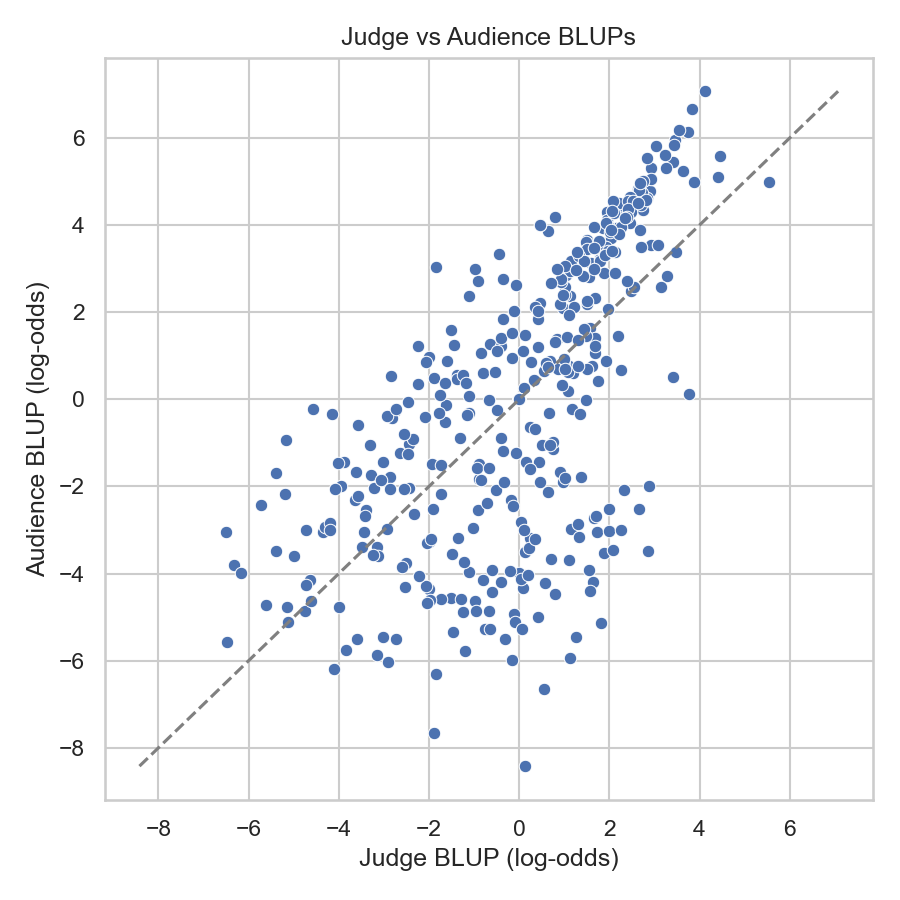
\includegraphics[width=0.95\linewidth]{output/fig/task3/cooperate_influence.png}
        \caption{Influence of different dancers on final rankings.}
        \label{fig:dancer_influence}
    \end{subfigure}
    \hfill  % 子图间自动填充空白（比 \quad 更适配双列）
    % 子图2：明星年龄对最终排名的影响
    \begin{subfigure}{0.48\textwidth}
        \centering
        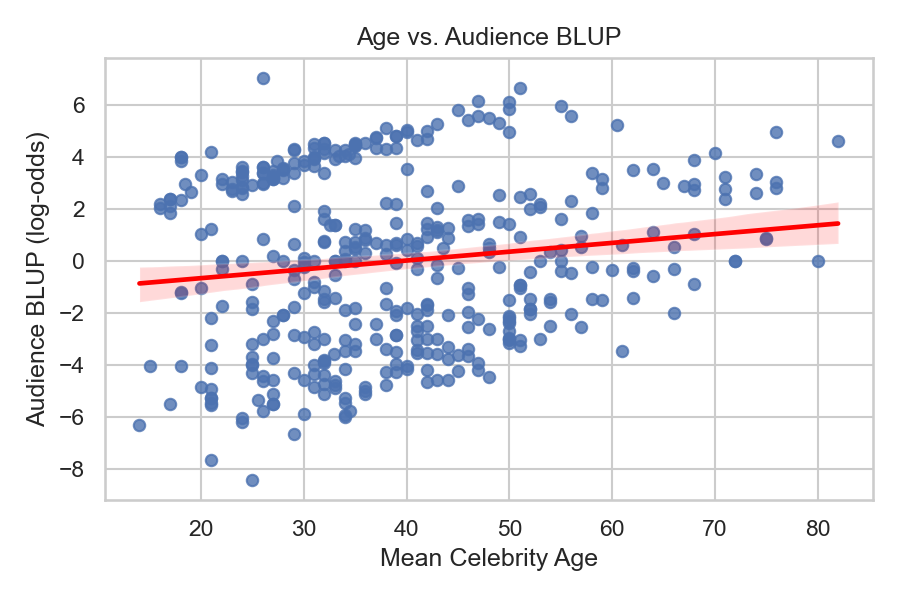
\includegraphics[width=0.95\linewidth]{output/fig/task3/age_influence.png}
        \caption{Influence of celebrity age on final rankings.}
        \label{fig:age_influence}
    \end{subfigure}
    
    % 总图标题（概括所有子图核心内容）
    \caption{Impacts of Dancer and Celebrity Age on Competition Final Rankings}
    % 总图标签（用于全文引用）
    \label{fig:rankings_influence}
\end{figure}
Such differences are practically attributed to a series of factors including experience and age; however, 
due to the lack of corresponding supporting data in the provided dataset, we do not conduct an in-depth analysis thereof.
\subsection{Impact of Celebrity Characteristics}
We calculate the trait preferences for relevant indicators of celebrities and obtain statistically significant results. Herein, we select age, industry, and other factors of celebrities for analysis.
\paragraph{Age}

In Tabel~\ref{fig:age_influence}, we find that older celebrities exhibit a stronger tendency to receive fan votes. That may be because older celebrities have a more established fan base and greater social influence, leading to higher vote counts.

\paragraph{Industry}
\begin{figure}[H]
    \centering
    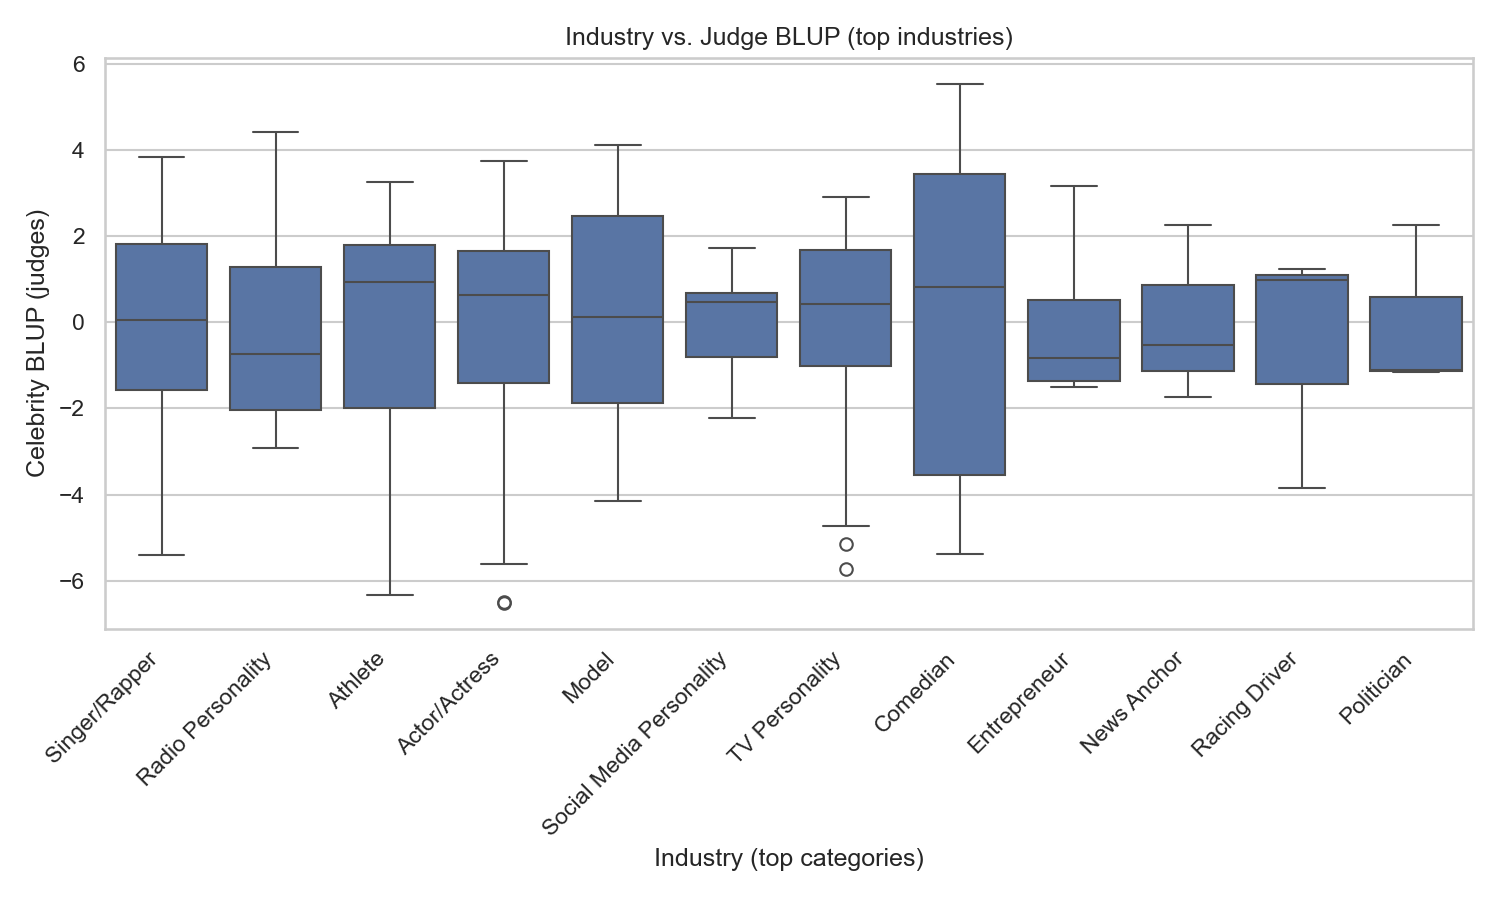
\includegraphics[width=0.95\linewidth]{output/fig/task3/industry_influence.png}
    \caption{Influence of celebrity industry on final rankings.}
    \label{fig:industry_influence}
\end{figure}
We find that different industries have a significant impact on final rankings. Among these, industries listed in Table~\ref{fig:industry_influence}, exert a significant positive effect on overall performance, while others tend to have less positive effect on overall performance.
\paragraph{Other Factors}
Differences in factors such as a celebrity's personal influence, dance foundation, and learning ability do exist and exert an impact in real scenarios. Thus, we argue that celebrities with greater personal influence, a solid dance foundation, and strong learning ability tend to achieve better performance. Nevertheless, these factors cannot be identified in the current dataset, and therefore we do not provide a quantitative interpretation thereof.


% ---------------- Figure/Table placeholders (insert later) ----------------
% Fig 6.1 Coefficient comparison (beta vs gamma) for key attributes.
% Fig 6.2 Preference gaps Delta_k with CI (bootstrap).
% Tab 6.1 ICC^{J}_{pro} and ICC^{V}_{pro} (overall + by era if desired).
% Tab 6.2 Top/bottom 5 pros by BLUP for judges and fans (side-by-side).
% ------------------------------------------------------------------------

% ======================================================================
% Chapter 6 Figures/Tables Placeholders (to be filled after model runs)
% Place this block at the END of:
%   6_impact_analysis_task_d1_pro_dancer_and_attributes.tex
% ======================================================================

% -----------------------------
% What MUST be backed by outputs (writing guardrails)
% -----------------------------
% Any claim of the form:
%   - "fans prefer X more than judges" / "judges reward X more"
%   - "gamma_J is significant/strong/weak"
%   - "pro dancer effect is large/non-negligible"
%   - "top/bottom pro dancer rankings"
% MUST be supported by the corresponding figure/table below.
% Otherwise hedge language: "we quantify / we evaluate / we report".

% % ======================================================================
% % FIGURE 6.1  Coefficient comparison (Judges vs Fans): beta_k vs gamma_k
% % ======================================================================
% % Purpose (MCM): show, at a glance, whether each attribute pushes judges and fans
% % in the same direction and with similar magnitude.
% % Inputs: model6_judge_coeffs.csv (beta, CI); model6_vote_coeffs.csv (gamma, CI)
% % Recommended: horizontal dot/interval plot, one row per feature, two series.
% % Insert in text: after the paragraph introducing the two models (Section 6.2).
% \begin{figure}[H]
%     \centering
%     %\includegraphics[width=0.95\linewidth]{figures/fig6_1_coef_compare.pdf}
%     \fbox{\parbox{0.95\linewidth}{\centering Placeholder: Fig 6.1 Coefficient comparison ($\beta_k$ vs $\gamma_k$)}}
%     \caption{Attribute effects in the Judge Model ($\beta_k$) versus the Vote Model ($\gamma_k$) on the log-odds scale (with 95\% confidence intervals).}
%     \label{fig:coef_compare_beta_gamma}
% \end{figure}

% % ======================================================================
% % FIGURE 6.2  Preference gap: Delta_k = gamma_k - beta_k (with uncertainty)
% % ======================================================================
% % Purpose (MCM): directly answers "who values what more" and supports any
% % narrative about preference differences.
% % Inputs: computed Delta_k table with CI from bootstrap or uncertainty propagation.
% % Insert in text: immediately after Fig 6.1 and the definition of Delta_k.
% \begin{figure}[H]
%     \centering
%     %\includegraphics[width=0.90\linewidth]{figures/fig6_2_delta_ci.pdf}
%     \fbox{\parbox{0.90\linewidth}{\centering Placeholder: Fig 6.2 Preference gaps ($\Delta_k$) with CI}}
%     \caption{Preference gaps $\Delta_k=\gamma_k-\beta_k$ for shared attributes. Positive values indicate stronger fan preference than judges; negative values indicate stronger judge preference (95\% confidence intervals via uncertainty propagation).}
%     \label{fig:delta_k_ci}
% \end{figure}

% % ======================================================================
% % TABLE 6.1  Variance components and ICC for pro-dancer effects
% % ======================================================================
% % Purpose (MCM): quantify magnitude (not just significance) of pro-dancer impact
% % on judges and fans. Supports statements like "pro accounts for X% variance".
% % Inputs: model6_variance_components.csv; compute ICC^J_pro and ICC^V_pro.
% % Insert in text: in Section 6.2 paragraph "Quantifying pro-dancer impact".
% \begin{table}[H]
%     \centering
%     %\input{tables/tab6_1_icc.tex}
%     \caption{Variance components and ICC-style ratios quantifying professional-dancer influence on judges' scores and inferred fan votes.}
%     \label{tab:icc_pro_effect}
% \end{table}

% % ======================================================================
% % TABLE 6.2  Pro-dancer BLUP rankings (Judges vs Fans), Top/Bottom 5
% % ======================================================================
% % Purpose (MCM): interpretable ranking of pros; supports case narratives and memo.
% % Inputs: BLUP random effects from Judge Model (v_pro) and Vote Model (b_pro).
% % Insert in text: after discussing BLUP interpretation and ICC results.
% \begin{table}[H]
%     \centering
%     %\input{tables/tab6_2_blup_top_bottom.tex}
%     \caption{Top and bottom professional dancers by fitted random effects (BLUPs), shown separately for judges' scores and inferred fan votes. Rankings are descriptive summaries of the fitted models.}
%     \label{tab:blup_pro_rankings}
% \end{table}

% % ======================================================================
% % OPTIONAL FIGURE 6.3  Transmission strength gamma_J (robustness / bootstrap)
% % ======================================================================
% % Purpose (MCM): make the "judges -> fans" transmission interpretable and robust.
% % Inputs: bootstrap_gamma_summary.csv (distribution of gamma_J across bootstrap runs)
% % Insert in text: after interpreting gamma_J in Vote Model.
% \begin{figure}[H]
%     \centering
%     %\includegraphics[width=0.75\linewidth]{figures/fig6_3_gammaJ_bootstrap.pdf}
%     \fbox{\parbox{0.75\linewidth}{\centering Optional: Fig 6.3 Bootstrap distribution of $\gamma_J$}}
%     \caption{Bootstrap distribution of the transmission coefficient $\gamma_J$ linking judges' evaluations to inferred fan votes.}
%     \label{fig:gammaJ_bootstrap}
% \end{figure}

% % ======================================================================
% % OPTIONAL TABLE 6.3  Model specification checklist (for reproducibility)
% % ======================================================================
% % Purpose (MCM): a compact audit table (FE, RE, trend, uncertainty method).
% % Insert in appendix if page-limited; keep here as optional.
% \begin{table}[H]
%     \centering
%     %\input{tables/tab6_3_model_spec_checklist.tex}
%     \caption{(Optional) Specification checklist for the Judge Model and Vote Model (fixed effects, random effects, week trend, season FE, and uncertainty propagation choice).}
%     \label{tab:model_spec_checklist}
% \end{table}

% % ======================================================================
% % Notes for the team (implementation mapping)
% % ======================================================================
% % Required artifacts to generate:
% % - figures/fig6_1_coef_compare.pdf  (beta vs gamma with CI)
% % - figures/fig6_2_delta_ci.pdf      (Delta_k with CI)
% % - tables/tab6_1_icc.tex            (variance components + ICC)
% % - tables/tab6_2_blup_top_bottom.tex (BLUP top/bottom 5)
% % Optional:
% % - figures/fig6_3_gammaJ_bootstrap.pdf
% % - tables/tab6_3_model_spec_checklist.tex
% % ======================================================================


\section{Task D-2: New Rule Design and Stress Testing}\label{sec:D2}
\subsection{Task D-2: New Rule Design and Stress Testing}
\label{subsec:task_d2}

\subsubsection{Design objective: professionalism-first, watchability as a constrained secondary goal}
\label{subsubsec:d2_objective}

Because DWTS is fundamentally a performance competition, we adopt a \emph{professionalism-first} rule design principle:
eliminations should be predominantly driven by judges' performance signals. At the same time, DWTS is a televised product,
so the system must preserve watchability by keeping a meaningful audience role and maintaining suspense.
Importantly, any additional uncertainty must remain \emph{performance-grounded} (induced by explicit rule structure operating on low performers),
rather than arbitrary randomness.

\paragraph{Operational definitions.}
We define \textbf{professionalism} as the extent to which eliminated contestants are concentrated in the lower tail of the weekly judges' ranking.
We define \textbf{watchability} as a constrained secondary objective that requires (i) a non-trivial marginal effect of fan votes on survival
(audience influence) and (ii) suspense that avoids overly deterministic outcomes, while remaining performance-grounded.

\paragraph{Notation.}
For each season--week $(s,t)$, let $q^J_{i,t}$ denote contestant $i$'s normalized judges' score share within the active set,
and let $p_{i,t}$ denote the inferred/proxy fan vote share from Task~A.
For a weight parameter $w_J\in[0,1]$, define a combined score
\[
S_{i,t}=w_J\,q^J_{i,t} + (1-w_J)\,p_{i,t}.
\]


\subsubsection{Rule A (incumbent baseline): combined score determines elimination}
\label{subsubsec:d2_ruleA}

Rule A represents the show's baseline mechanism, in which judges' scores and fan votes are combined into a single weekly
decision score, and elimination is determined directly by that combined ordering:
\begin{enumerate}
  \item Compute $S_{i,t}$ for all active contestants.
  \item Eliminate the contestant with the lowest $q^J_{i,t}$.
\end{enumerate}
This baseline can preserve audience influence when fan weights are large, but it also permits ``popularity-only'' survival:
a contestant with weak judges' performance may avoid elimination if fan support is sufficiently strong, which can weaken professionalism.


\subsubsection{Rule B (proposed): judges-only gating $\rightarrow$ fan-aware decision within the risk set}
\label{subsubsec:d2_ruleB}

Our proposed institutional change is a \emph{two-stage gate-and-decide} mechanism that makes professionalism structural:
judges alone define who is at risk, and fan influence is applied only within that performance-defined boundary.

\begin{enumerate}
  \item \textbf{Judges-only gate (risk set).} Rank contestants by judges' performance $q^J_{i,t}$ and let
  $B^J_t$ be the Bottom-2 under judges (Judge Bottom-2).
  \item \textbf{Fan-aware decision within the gate.} Within $B^J_t$, compute $S_{i,t}$ and eliminate the contestant with the lower combined score:
  \[
  \tilde{E}_{s,t}=\arg\min_{i\in B^J_t} \big(w_J\,q^J_{i,t} + (1-w_J)\,p_{i,t}\big).
  \]
\end{enumerate}

\paragraph{Why Rule B improves professionalism.}
By construction, elimination is always decided among the lowest-performing contestants according to judges.
This prevents extreme popularity from overriding performance signals outside the judges-defined bottom tail,
thereby strengthening professionalism, especially in early weeks when performance dispersion is largest.

\paragraph{Maintaining watchability without randomness: phase-dependent structured suspense.}
Because DWTS features celebrity participants, early-season skill gaps can be large and a strict professionalism-first gate may reduce
perceived audience impact. We therefore treat watchability as a constrained secondary goal and introduce \emph{structured suspense} only in late stages,
while maintaining performance grounding:
\begin{itemize}
  \item \textbf{Late-stage bottom-$k$ band (within judges' tail).}
  When the field is small (e.g., remaining contestants $\le K$), expand the judges-defined risk set from Bottom-2 to Bottom-$k$,
  and decide elimination within that band using $S_{i,t}$. This widens the decision boundary and increases suspense without leaving the low-performance region.
  \item \textbf{Limited structured multi-elimination (optional).}
  In a small number of late-stage weeks, allow multi-elimination, but restrict eliminations to the judges-defined bottom band.
  This increases stakes while remaining performance-grounded.
\end{itemize}
The phase boundary ($K$ or a week threshold $t_0$) and the band size $k$ are interpretable management knobs.


\subsubsection{Stress testing via replay}
\label{subsubsec:d2_stress}

What kind of stress test we employed to evaluate Rule B and select parameters?

\paragraph{Parameter sweep (control knobs).}


\paragraph{Evaluation metrics (professionalism-first).}
We report:
\begin{itemize}
  \item \textbf{Professionalism proxy: judges-tail alignment.}
  The eliminated contestant's weekly judges' rank/quantile distribution (greater concentration in the lower tail indicates higher professionalism).
  \item \textbf{Replay consistency (KPI1).}
  Week-level elimination-set agreement between observed and replayed outcomes (Jaccard mean under our stated convention).
  \item \textbf{Structured suspense proxy (KPI3 / FlipRate).}
  The rate at which elimination outcomes change across rules/parameters, capturing how institutional design introduces suspense.
  \item \textbf{Audience influence proxy.}
  Sensitivity of elimination outcomes to perturbations of $p_{i,t}$ within the feasible uncertainty range from Task~A.
\end{itemize}

\paragraph{Robustness checks.}
We conduct those robustness checks:


\noindent In summary, Rule B makes professionalism a structural property through judges-only gating, while late-stage structured mechanisms
preserve watchability without introducing randomness. Replay-based stress testing provides an interpretable policy region rather than a single tuned setting.


\section{Conclusion}\label{sec:conclusion}
We model \emph{Dancing with the Stars} as a replayable inverse problem: judges' scores and eliminations are observed,
while audience votes are latent. Task~A infers weekly fan vote shares consistent with observed exits and reports
identifiability/uncertainty; Tasks~B--C use these inferred votes to replay eliminations across seasons to quantify how
aggregation mechanics (rank vs.\ percent) and the incumbent Bottom-2 + judges' save safeguard change outcomes. Any
completion needed when a counterfactual keeps an observed-exit contestant active is handled conservatively for replay
closure only (not for forecasting).

Building on the inferred fan signal and mechanism interpretation (Task~D1), Task~D2 proposes \emph{Professional Bottom-2} (PB2):
judges first define a small performance-grounded risk set, and fan influence is applied only within that gate via a
transparent weighted blend. PB2 preserves audience agency while reducing extreme reversals, and we validate it through
replay-based stress tests (stability across rules and seasons, controversial-case replays, and a unified bias check).

Overall, the pipeline provides an auditable chain from cleaned data to interpretable mechanisms to actionable rule
recommendations, while explicitly flagging weeks/seasons where non-identifiability limits confidence. Future work can
incorporate additional popularity signals and evaluate alternative safeguards within the same replay-and-stress-test
framework.


\section{Memo to Management}\label{sec:memo}
\textbf{To: Show Management}\\
\textbf{Subject: Recommendation for a More Professional Yet Watchable Voting System}

Our analyses indicate that controversy risk concentrates in weeks where judges' evaluations and audience preferences diverge.
To prioritize technical merit while preserving an audience role, we recommend piloting \textit{Professional Bottom-2} (\textit{PB2}), a judges-gated two-stage voting policy,
validated by replay-based stress tests: (i) pairwise Jaccard similarity across Percent/Rank/B2/PB2, (ii) controversial-case replays, and (iii) a unified bias test.

\paragraph{Baseline reference (current mechanism).}
The incumbent format can be summarized as ``combined Bottom-2 + judges' save'': contestants are first ranked by a combined
judge--fan score, the Bottom-2 form an at-risk set, and judges decide which of the two is eliminated.

\paragraph{Recommended policy (PB2: \textit{Professional Bottom-2}): judges-only gate $\rightarrow$ fan-aware decision within the gate.}
Under PB2, each week proceeds in two stages:
\begin{enumerate}
  \item \textbf{Judges-only gate (risk set).} Rank contestants by judges' performance share $q^J_{i,t}$ and designate the Bottom-2
  (or Bottom-$k$ in late-stage variants) as the at-risk set.
  \item \textbf{Fan-aware decision within the gate.} Within the at-risk set, eliminate the contestant with the lower transparent blended score
  \[
  S_{i,t}=w_J\, q^J_{i,t} + (1-w_J)\, p_{i,t},
  \]
  where $p_{i,t}$ denotes the inferred/proxy fan vote share.
\end{enumerate}

\paragraph{Why this improves professionalism.}
Because elimination is always decided among the judges-defined bottom performers, extreme popularity cannot keep a weak performer
out of the at-risk set. This makes professionalism a structural property of the system rather than a tunable side effect.

\paragraph{How we preserve watchability (without randomness).}
To maintain suspense while remaining performance-grounded, we recommend a phase-dependent schedule:
early weeks use Bottom-2 gating to emphasize professionalism; late in the season (when remaining contestants are few and performance gaps narrow),
management may enable structured suspense by expanding the gate to a Bottom-$k$ band and/or using a small number of structured multi-elimination weeks,
with eliminations restricted to the judges-defined low-performance band.

\paragraph{Management knobs and deployment.}
PB2 offers interpretable control knobs:
(i) $w_J$ (judge--fan balance within the gate),
(ii) the late-stage trigger (e.g., remaining contestants $\le K$ or week threshold $t_0$),
and (iii) the late-stage gate size $k$ (and optional multi-elimination placement).
We recommend selecting a robust operating point supported by replay-based stress tests (Jaccard similarity, controversial-case replays, and a unified bias test), and deploying PB2 in a one-season
\emph{shadow mode} computed in parallel with the broadcast rule. This yields an auditable comparison of eliminations, finalists, and winner outcomes
before any on-air adoption, supported by a clear public explanation of the two-stage logic and the role of audience influence.



% =======================引用=========================
\bibliographystyle{IEEEtran}
\bibliography{chapters/myref}


% =======================附录=========================
\appendix
\section{Appendix: Data, Algorithms, and Reproducibility}\label{app:all}
\section*{Appendix 1: Cutoff Sensitivity Analysis}\label{appendix:cutoff_sensitivity_analysis}
In this appendix, we complete the cutoff sensitivity analysis for our rule-replay module discussed in Section~\ref{subsubsec:d2_stress}.
\begin{figure}[H]
  \begin{subfigure}{0.49\textwidth}
    \centering
    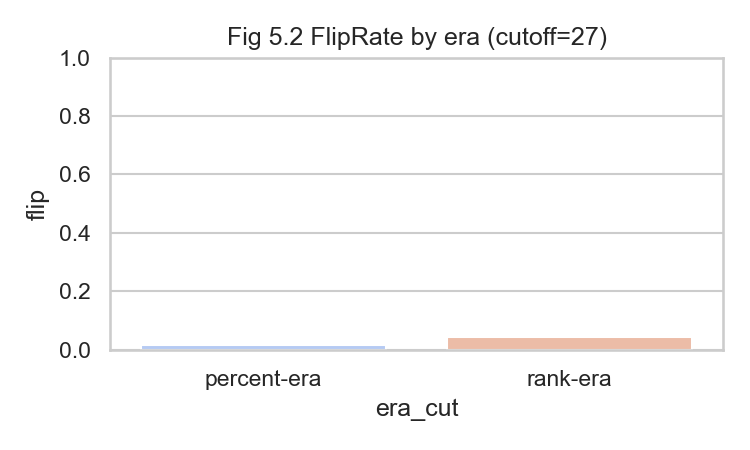
\includegraphics[width=\linewidth]{output/fig/fig5_2_cutoff_27_fliprate.png}
    \caption{Cutoff at Season-27.}
    \label{fig:cutoff_27}
  \end{subfigure}
  \hfill
  \begin{subfigure}{0.49\textwidth}
    \centering
    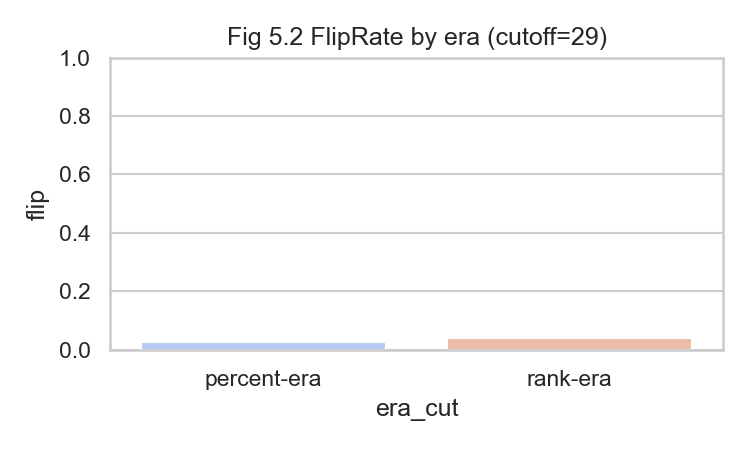
\includegraphics[width=\linewidth]{output/fig/fig5_2_cutoff_29_fliprate.png}
    \caption{Cutoff at Season-29.}
    \label{fig:cutoff_29}
  \end{subfigure}
\end{figure}

\section{Complete Files for Problem B}
See \href{https://github.com/charles65536/model2026-2}{2625838} for repository tree and executiomn steps.
\clearpage


% ==================================================================================
% Report on Use of AI (Appendix - NOT counted in main 25 pages if your rule allows)
% Place this at the very end of the appendices.
% ==================================================================================
\pagenumbering{gobble}
\begingroup
\setstretch{0.95}
\fontsize{9}{10.5}
\selectfont
\section*{\center{Report on Use of AI}}
\noindent\textbf{Team Control Number:} \# 2625838\\
\textbf{Problem:} C\\

\vspace{0.1em}
\subsection*{AI Tools Used}
\begin{table}[h!]
\centering
\small
\setlength{\tabcolsep}{6pt}
\renewcommand{\arraystretch}{1.15}
\begin{tabular}{|p{3.2cm}|p{3.2cm}|p{8.2cm}|}
\hline
\textbf{AI Tool} & \textbf{Version / Model} & \textbf{Primary Purpose} \\
\hline
OpenAI ChatGPT  & GPT-5.2 &
Language polishing, structural refinement, and clarification of written explanations \\
OpenAI ChatGPT & GPT-5.2 &
Brainstorming ideas for modeling approaches, algorithm designs, and solution strategies \\
OpenAI ChatGPT & GPT-5.2 &
Generating preliminary code drafts for data processing, graph producing and simulation, later reviewed and modified by the team \\
OpenAI ChatGPT & GPT-5.2 &
Synthesis of the explanatory documents, work orders, template tickets for internal team Delivery \\
OpenAI ChatGPT & GPT-5.2 &
Giving Advice on engineered Document Management and Version Control best practices \\
Github Copilot & \center{---} & Enhance productivity while maintaining full control over the code quality and integrity\\
\hline
\end{tabular}
\end{table}

\subsection*{Query/Response Record}
Click \textbf{ChatGPT Query \#} to view the full input and output records on GitHub. Screenshots of the outputs are provided below for reference.
\textbf{\href{https://github.com/charles65536/model2026-2/blob/main/report_on_use_of_ai/chatgpt_1_output.md}{ChatGPT Query 1:}}\\
\textbf{Input:}
We just inished our setting of \textit{dynamic\_files}, please refer to the \textit{first\_stage\_modeling.md} and \textit{context\_pack\_for\_ai.md} in our repository, 
and search for authorative and highly credible supporting literature on topics of convex optimization/scalable solving, underdetermined inversion/regularization, ranking/rule differences, compositional data, simulation and sensitivity\\
\textbf{Output:}
\begin{figure}[H]
  \centering
  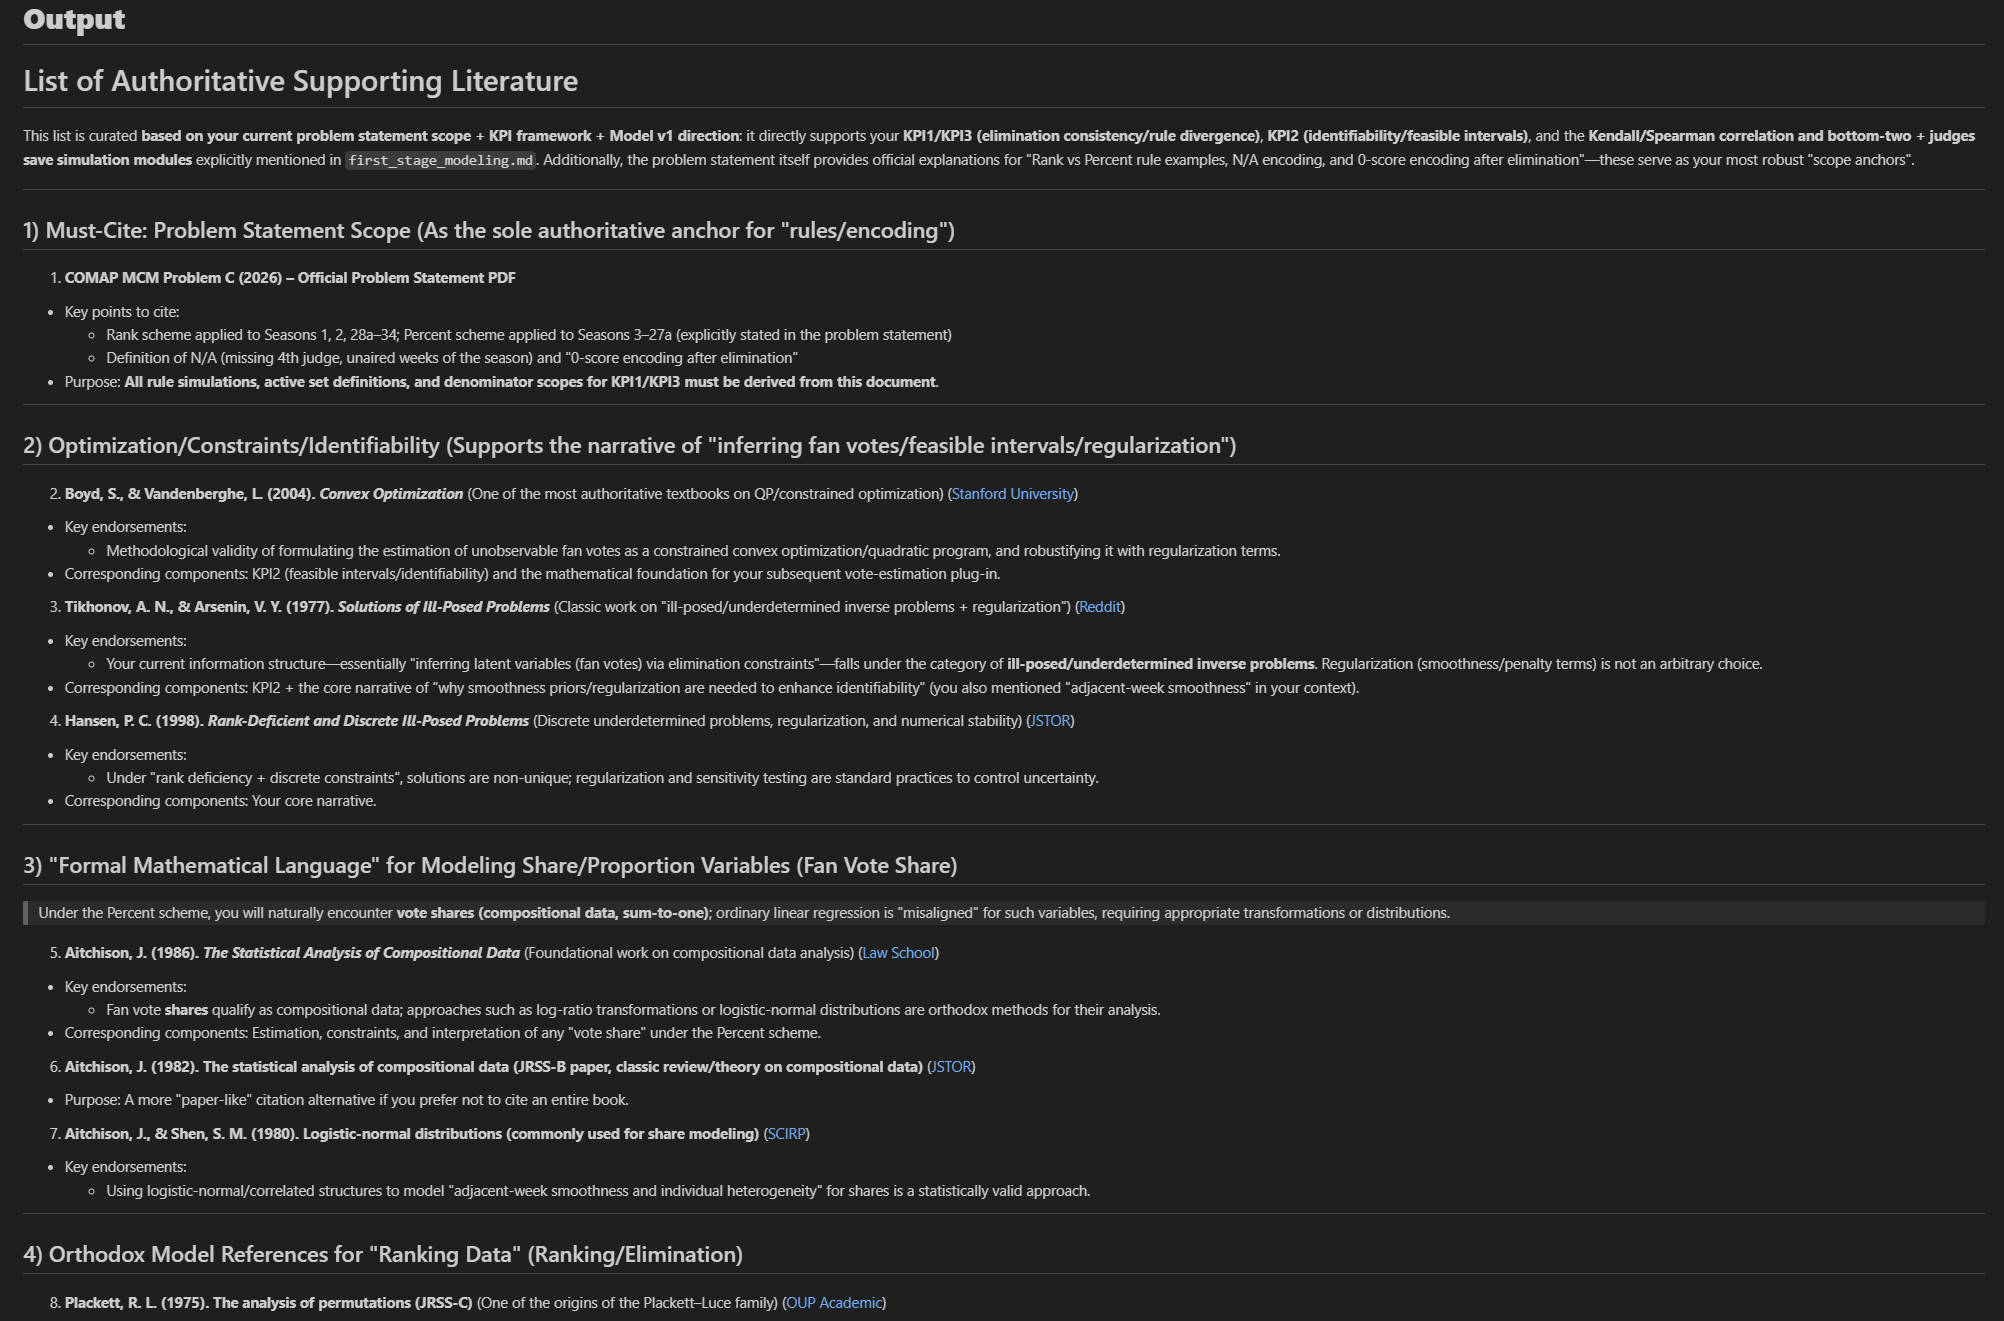
\includegraphics[width=0.9\linewidth]{report_on_use_of_ai/pho/1_1.png}
  \caption{ChatGPT Query 1 Output Screenshot}
  \label{fig:chatgpt_query_1_output}
\end{figure}
\begin{figure}[H]
  \centering
  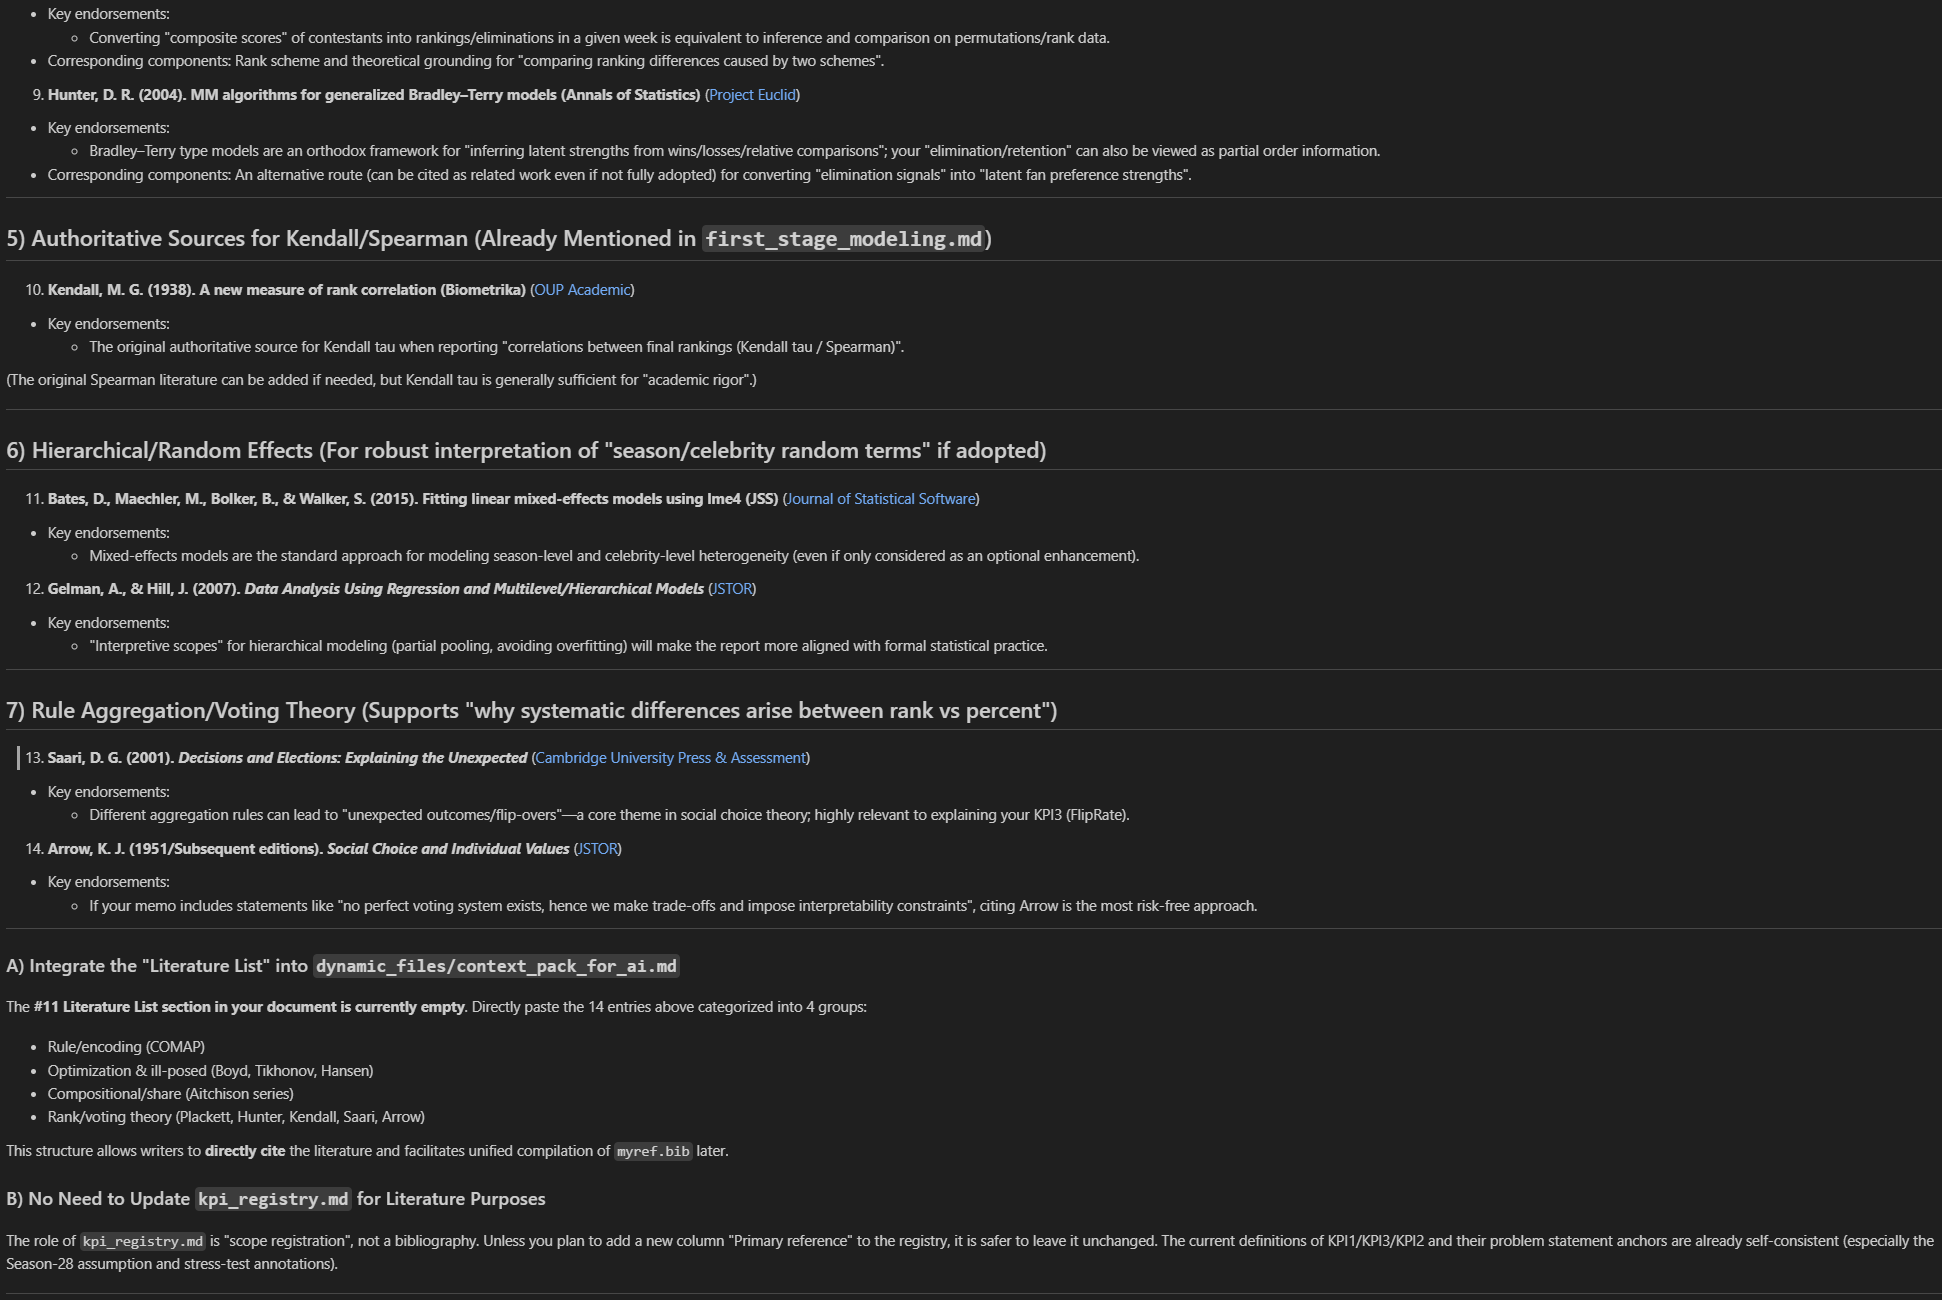
\includegraphics[width=0.9\linewidth]{report_on_use_of_ai/pho/1_2.png}
  \caption{ChatGPT Query 1 Output Screenshot (Continued)}
  \label{fig:chatgpt_query_1_output_2} 
\end{figure}

\textbf{\href{https://github.com/charles65536/model2026-2/blob/main/report_on_use_of_ai/chatgpt_2_input_and_output.md}{ChatGPT Query 2:}}\\
\begin{figure}[H]
  \centering
  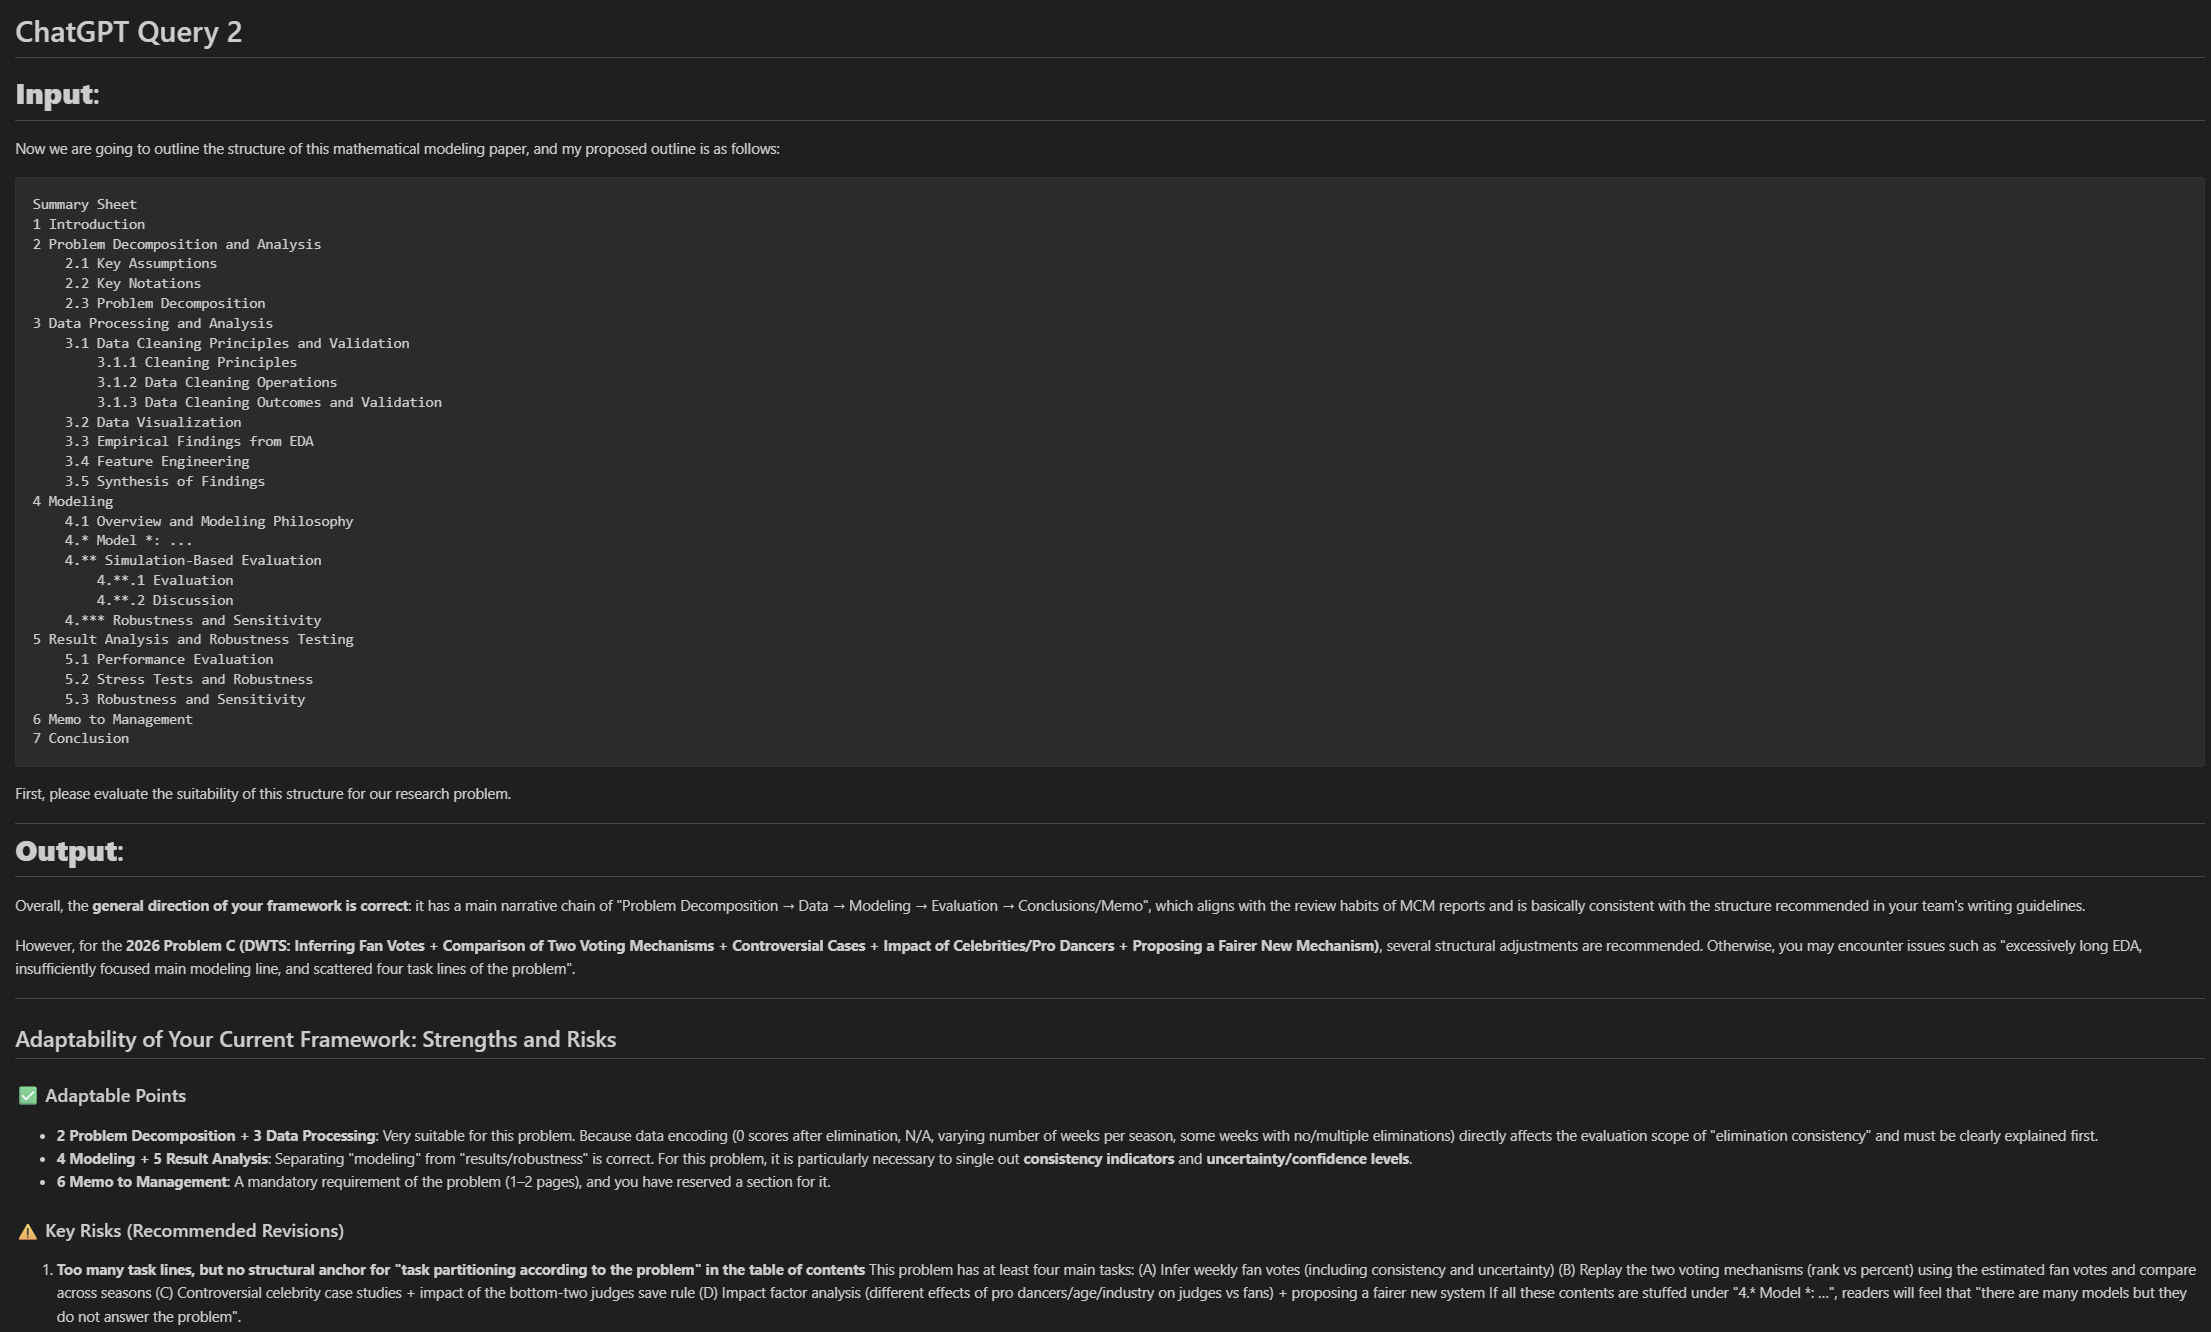
\includegraphics[width=0.9\linewidth]{report_on_use_of_ai/pho/2_1.png}
  \caption{ChatGPT Query 2 Output Screenshot}
  \label{fig:chatgpt_query_2_output}
\end{figure}
\begin{figure}[H]
  \centering
  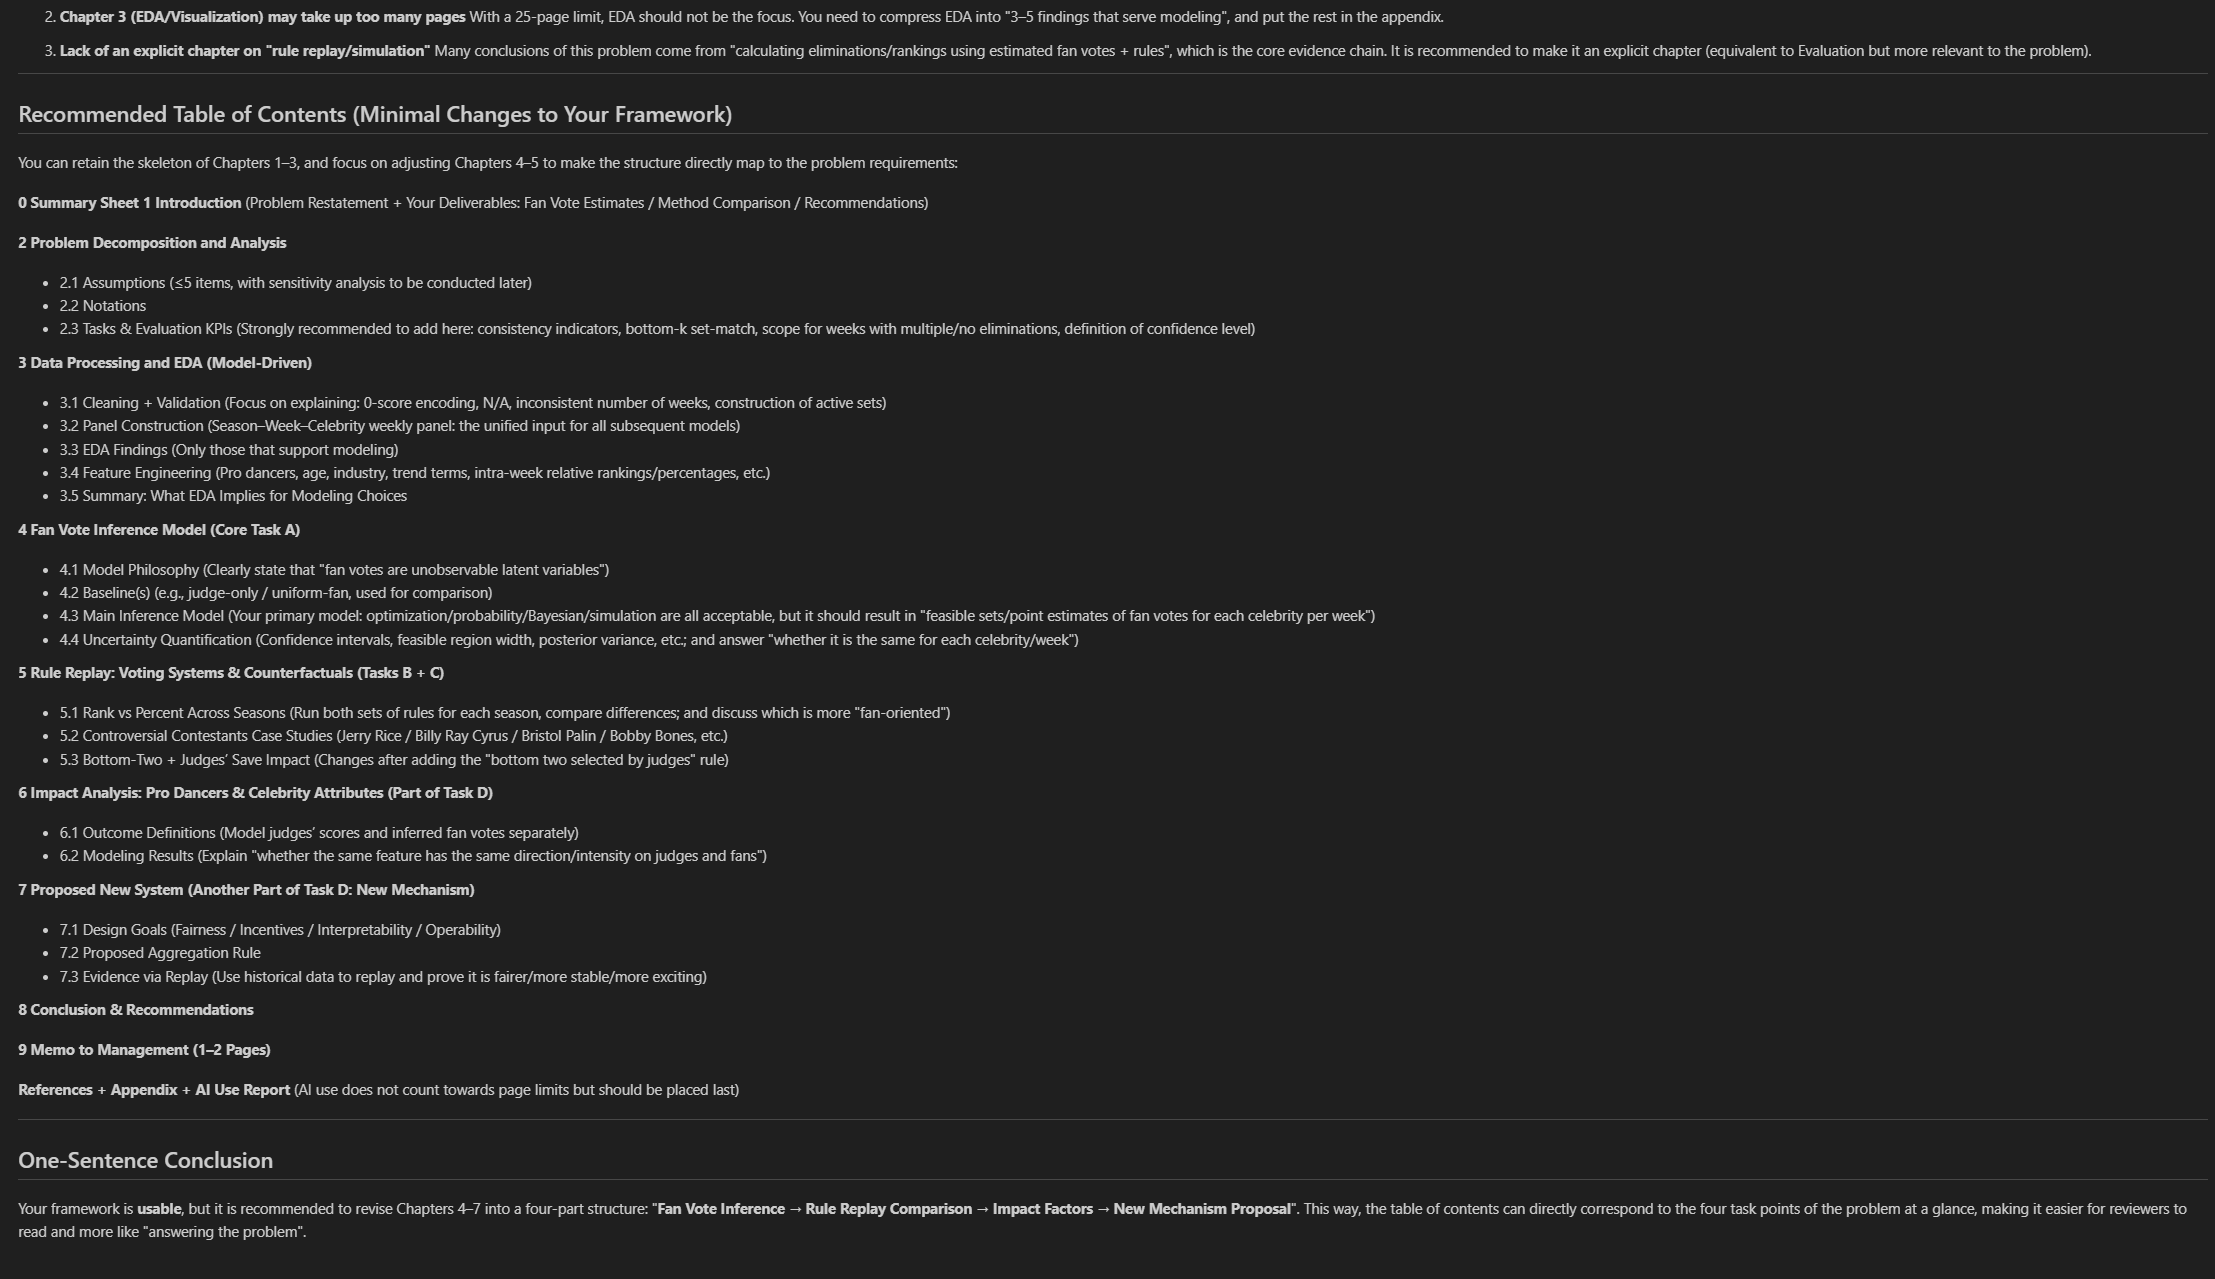
\includegraphics[width=0.9\linewidth]{report_on_use_of_ai/pho/2_2.png}
  \caption{ChatGPT Query 2 Output Screenshot (Continued)}
  \label{fig:chatgpt_query_2_output_2}
\end{figure}

\textbf{\href{https://github.com/charles65536/model2026-2/blob/main/report_on_use_of_ai/chatgpt_3_input_and_output.md}{ChatGPT Query 3:}}\\
\textbf{Input:}
\begin{figure}[H]
  \centering
  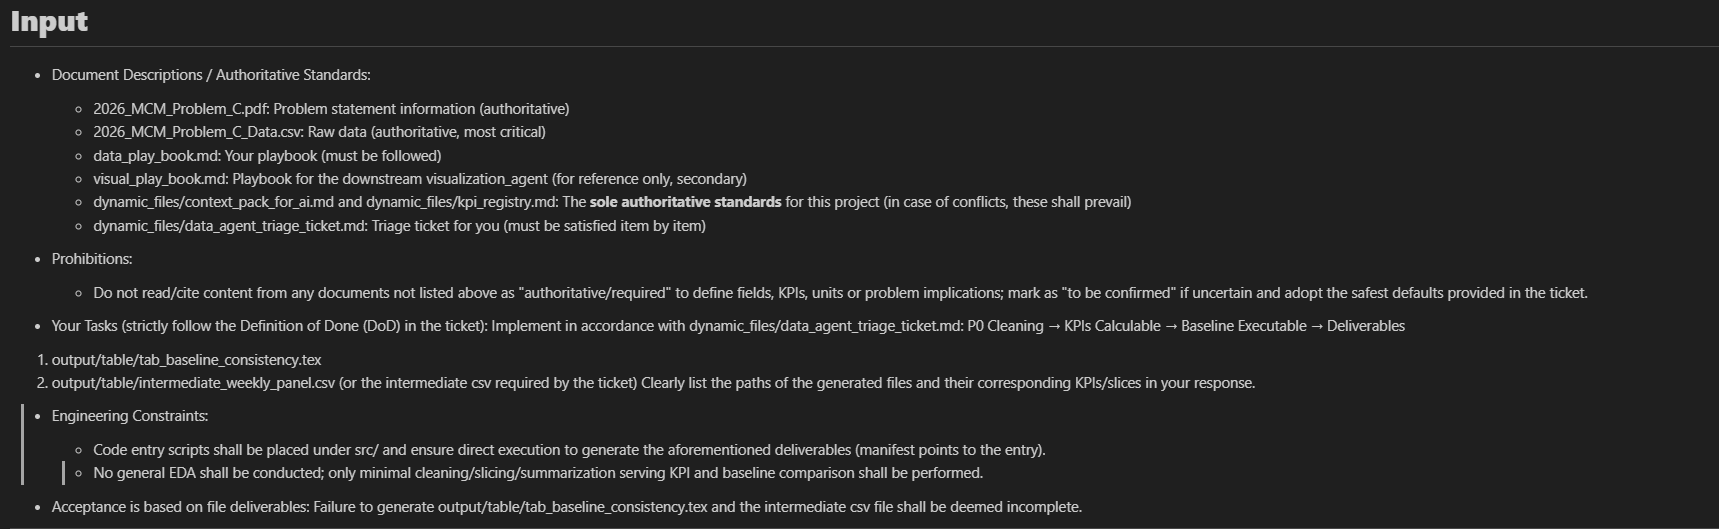
\includegraphics[width=0.9\linewidth]{report_on_use_of_ai/pho/3_1.png}
  \caption{ChatGPT Query 3 Input Screenshot}
  \label{fig:chatgpt_query_3_input}
\end{figure}
\textbf{Output:}
\begin{figure}[H]
  \centering
  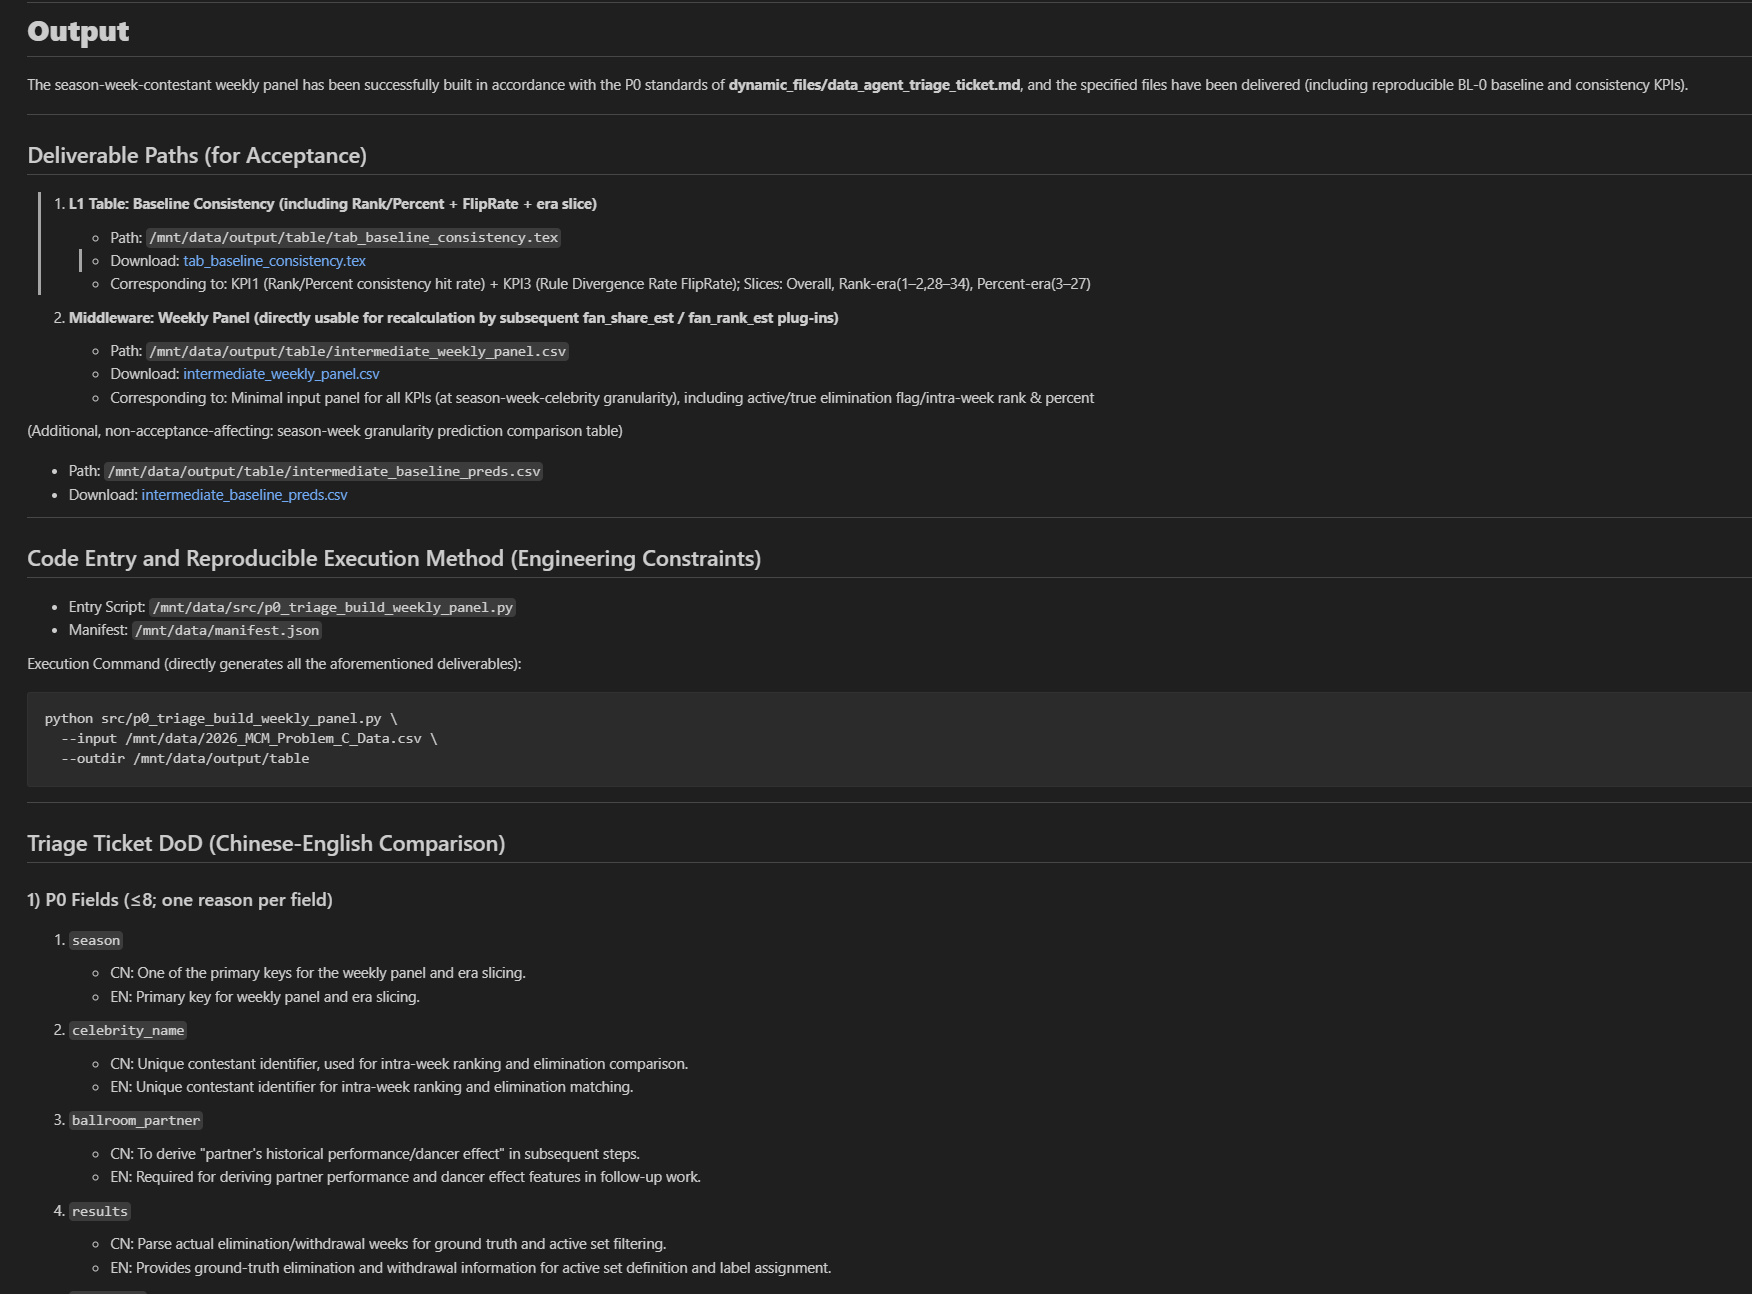
\includegraphics[width=0.9\linewidth]{report_on_use_of_ai/pho/3_2.png}
  \caption{ChatGPT Query 3 Output Screenshot}
  \label{fig:chatgpt_query_3_output}
\end{figure}
\begin{figure}[H]
  \centering
  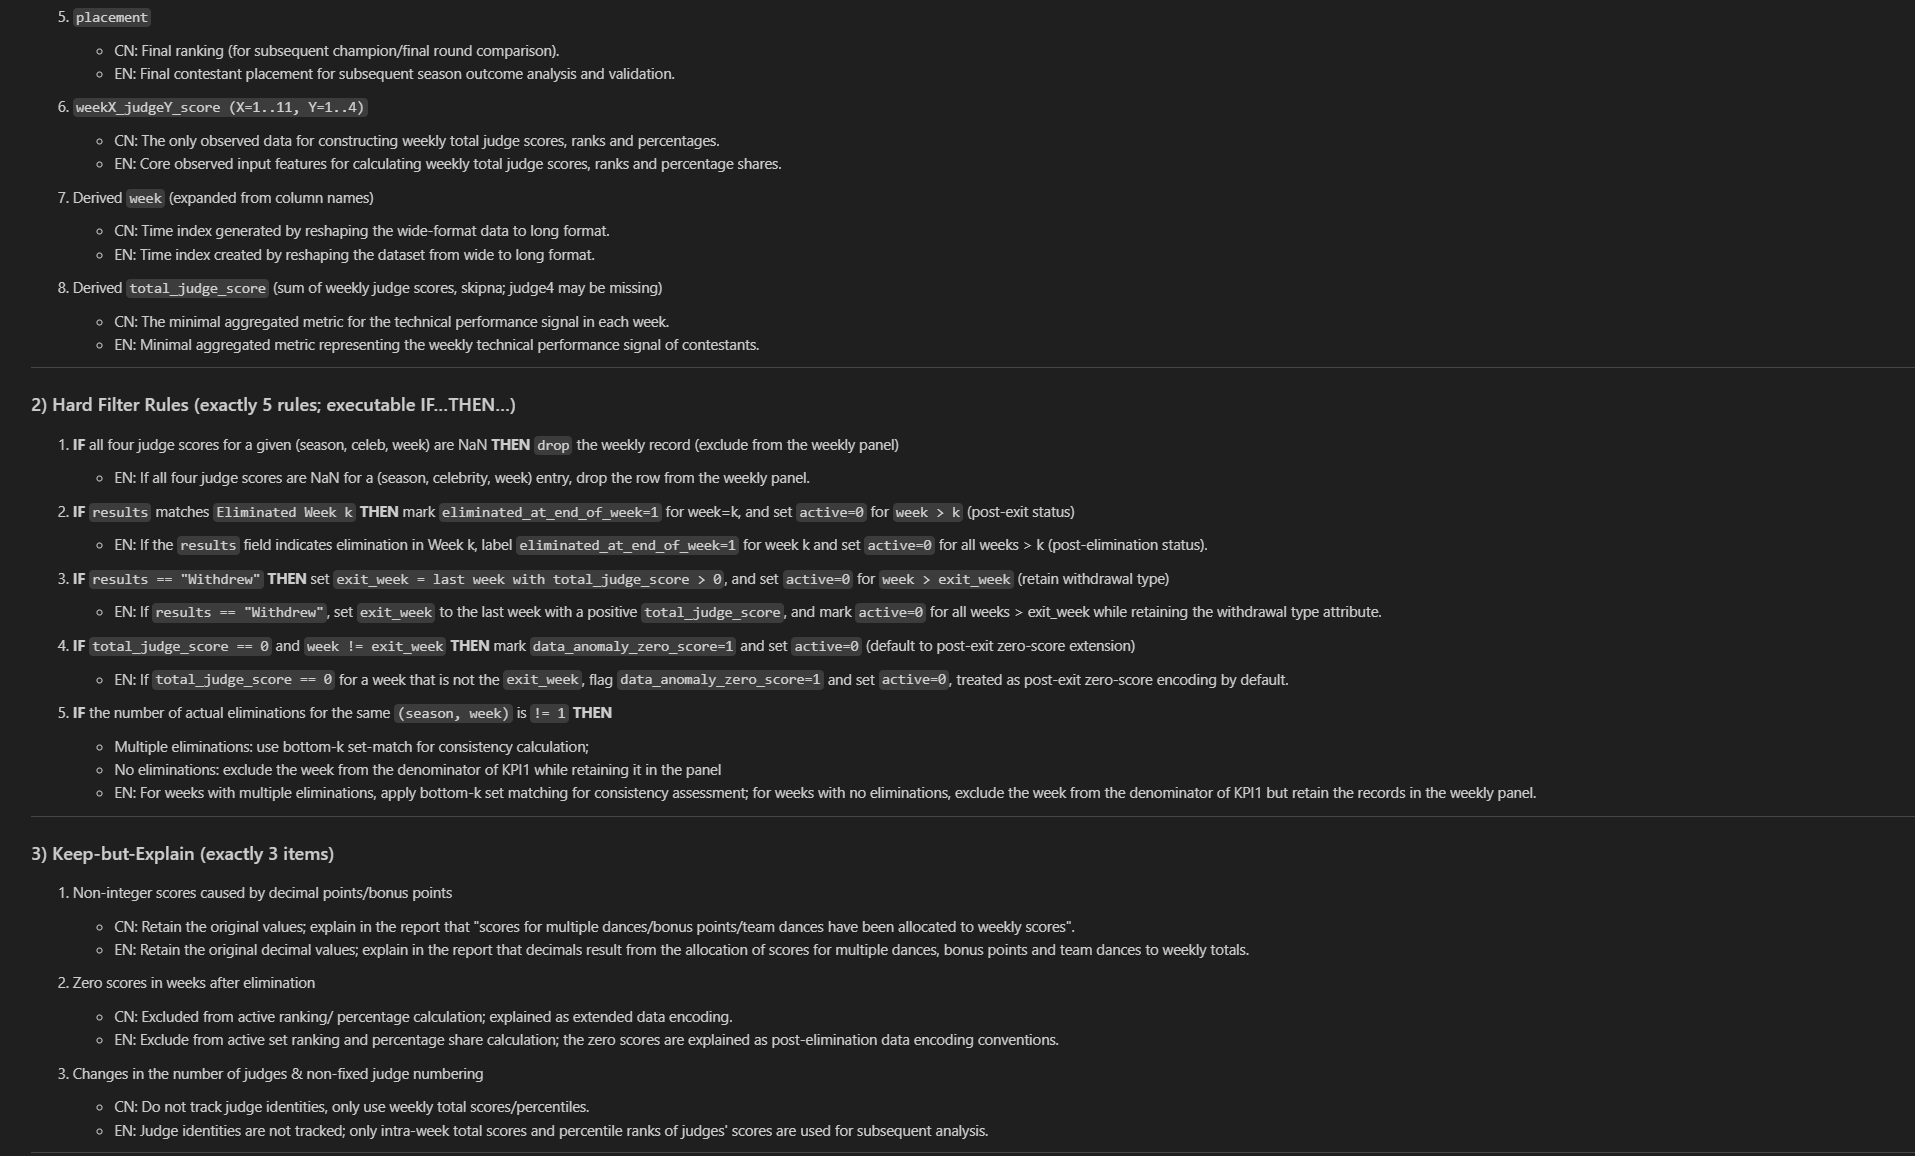
\includegraphics[width=0.9\linewidth]{report_on_use_of_ai/pho/3_3.png}
  \caption{ChatGPT Query 3 Output Screenshot (Continued)}
  \label{fig:chatgpt_query_3_output_2}
\end{figure}
\begin{figure}[H]
  \centering
  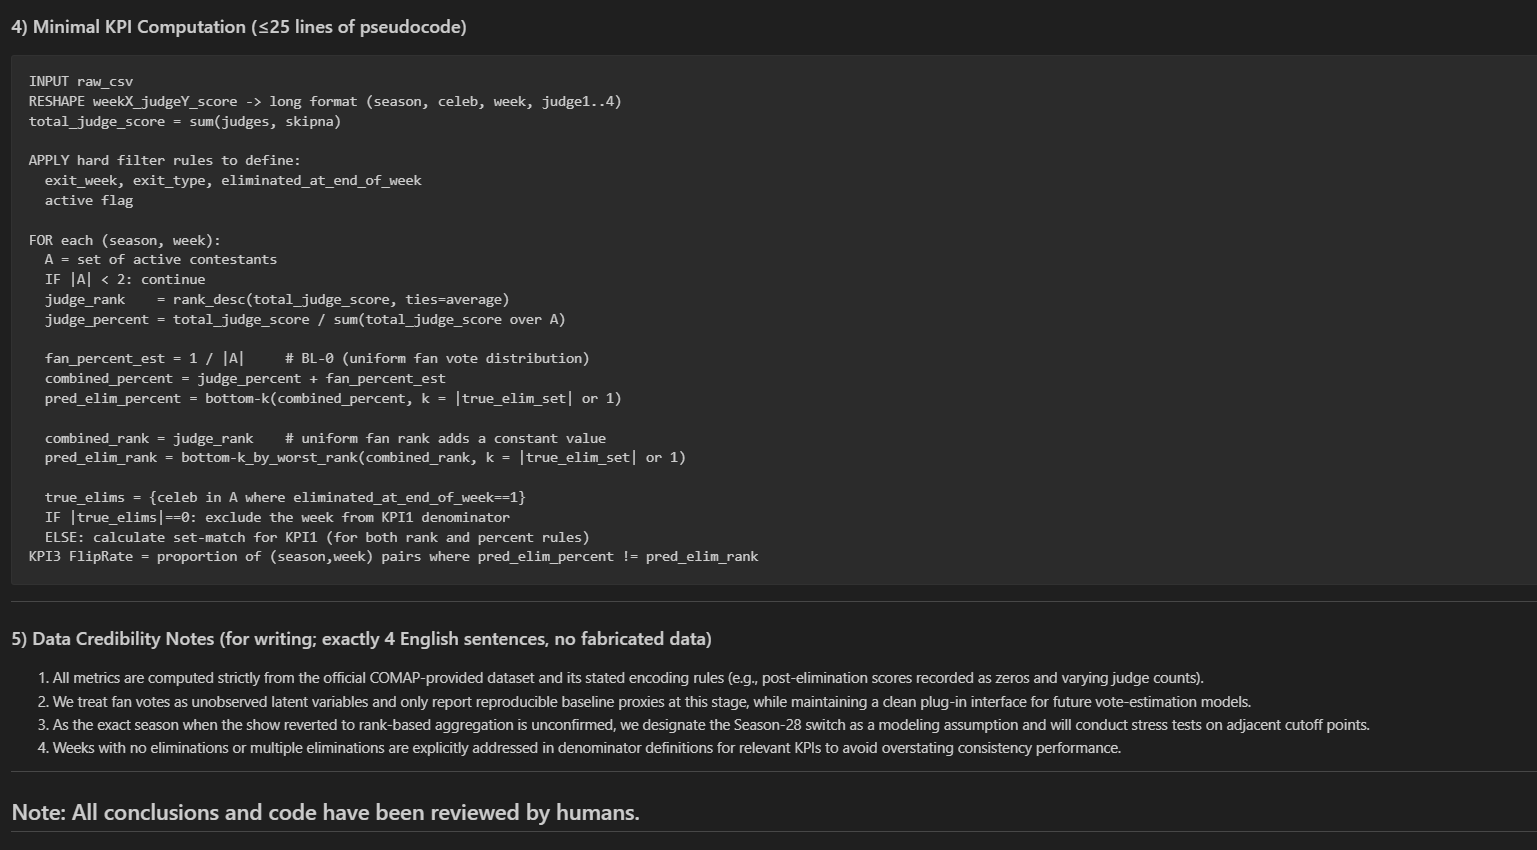
\includegraphics[width=0.9\linewidth]{report_on_use_of_ai/pho/3_4.png}
  \caption{ChatGPT Query 3 Output Screenshot (Continued)}
  \label{fig:chatgpt_query_3_output_3}
\end{figure}




\textbf{\href{https://github.com/charles65536/model2026-2/blob/main/report_on_use_of_ai/chatgpt_4_input_and_output.md}{ChatGPT Query 4:}}\\
\textbf{Input:}
Wait, why is the generated .pdf file completely unchanged? Could there be an issue with how we implemented the rules? Also, where in the code you provided do we need to modify the paths for importing and exporting files?\\
\textbf{Output:}
\begin{figure}[H]
  \centering
  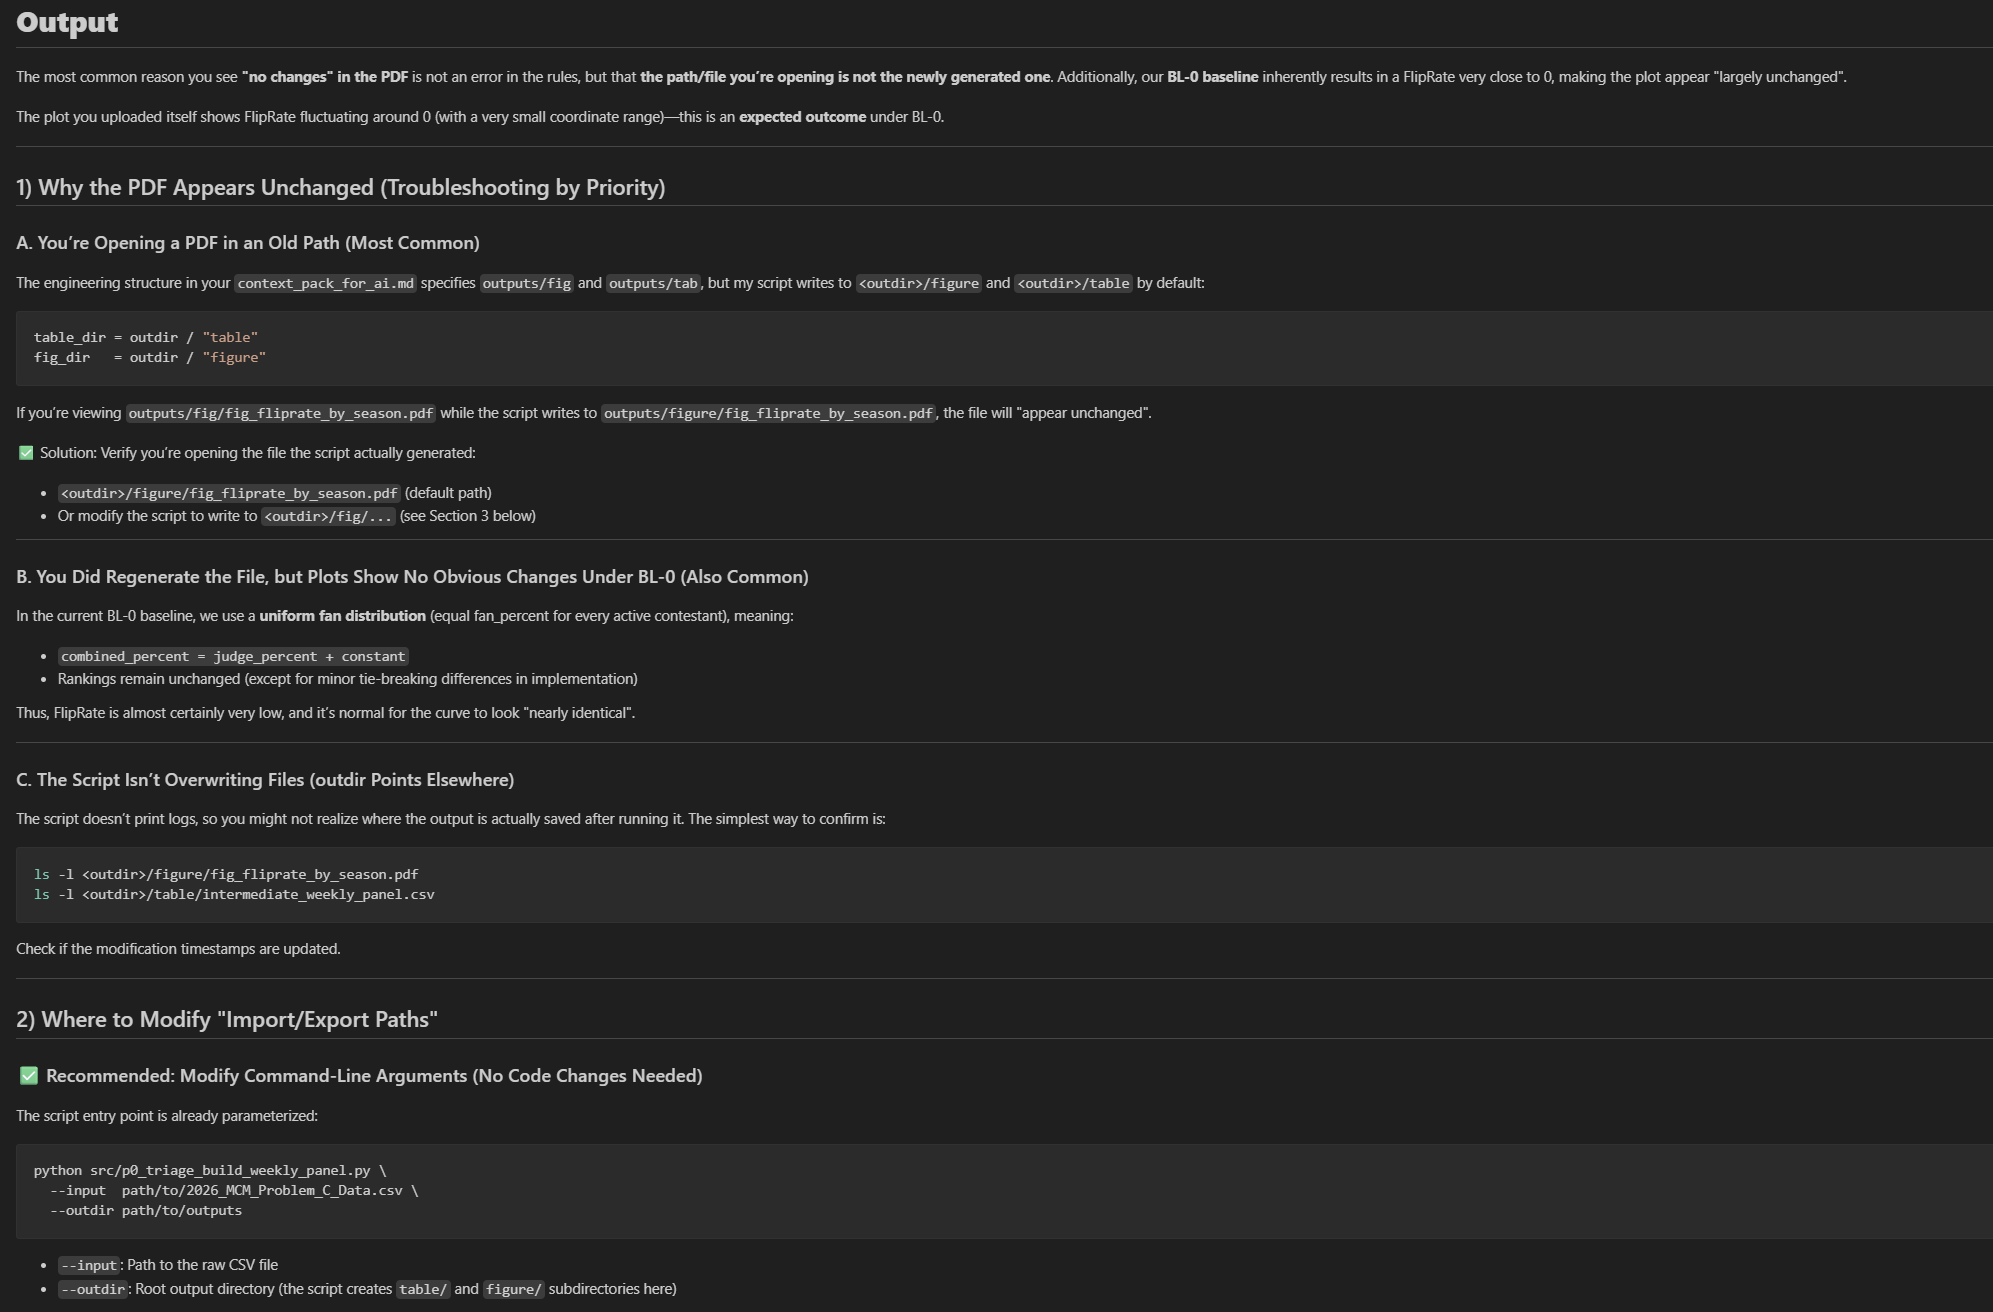
\includegraphics[width=0.9\linewidth]{report_on_use_of_ai/pho/4_1.png}
  \caption{ChatGPT Query 4 Output Screenshot}
  \label{fig:chatgpt_query_4_output}
\end{figure}
\begin{figure}[H]
  \centering
  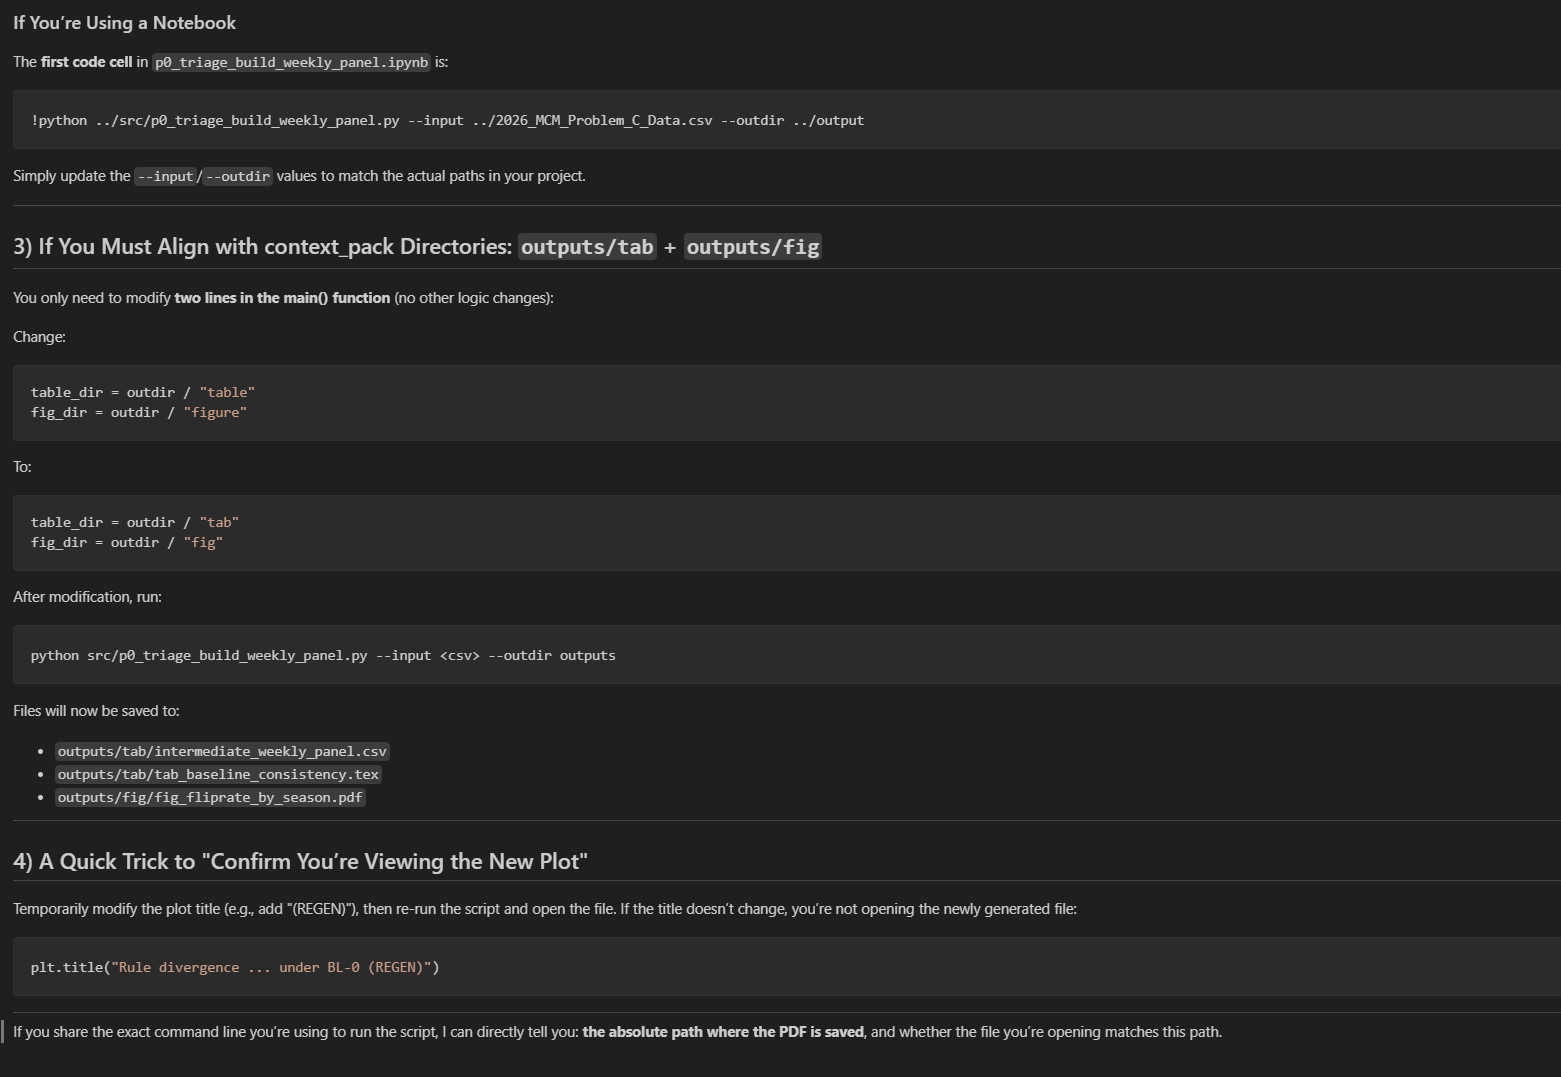
\includegraphics[width=0.9\linewidth]{report_on_use_of_ai/pho/4_2.png}
  \caption{ChatGPT Query 4 Output Screenshot}
  \label{fig:chatgpt_query_4_output_2}
\end{figure}


\textbf{\href{https://github.com/charles65536/model2026-2/blob/main/report_on_use_of_ai/chatgpt_5_input_and_output.md}{ChatGPT Query 5:}}\\
\textbf{Input:}
Currently, our .py code files are located at 2026\_MCM/src/LI\_play\_data/*.py, and we expect the generated charts to be saved to 2026\_MCM/output/fig (or 2026\_MCM/output/tab for tables, and the required data to be saved to 2026\_MCM/output/data\_cleaned).
I have several questions:\\
(a) Do we need to manually create the output/fig and output/tab directories in advance?\\
(b) If not, do we need to modify the paths in the Python files, and how? (We do not plan to use .ipynb files.)\\
(c) After modifying the paths in the files, how should I run the script on a Windows computer to generate the new files? Will the newly generated files overwrite the existing ones after running the script?\\
\textbf{Output:}
\begin{figure}[H]
  \centering
  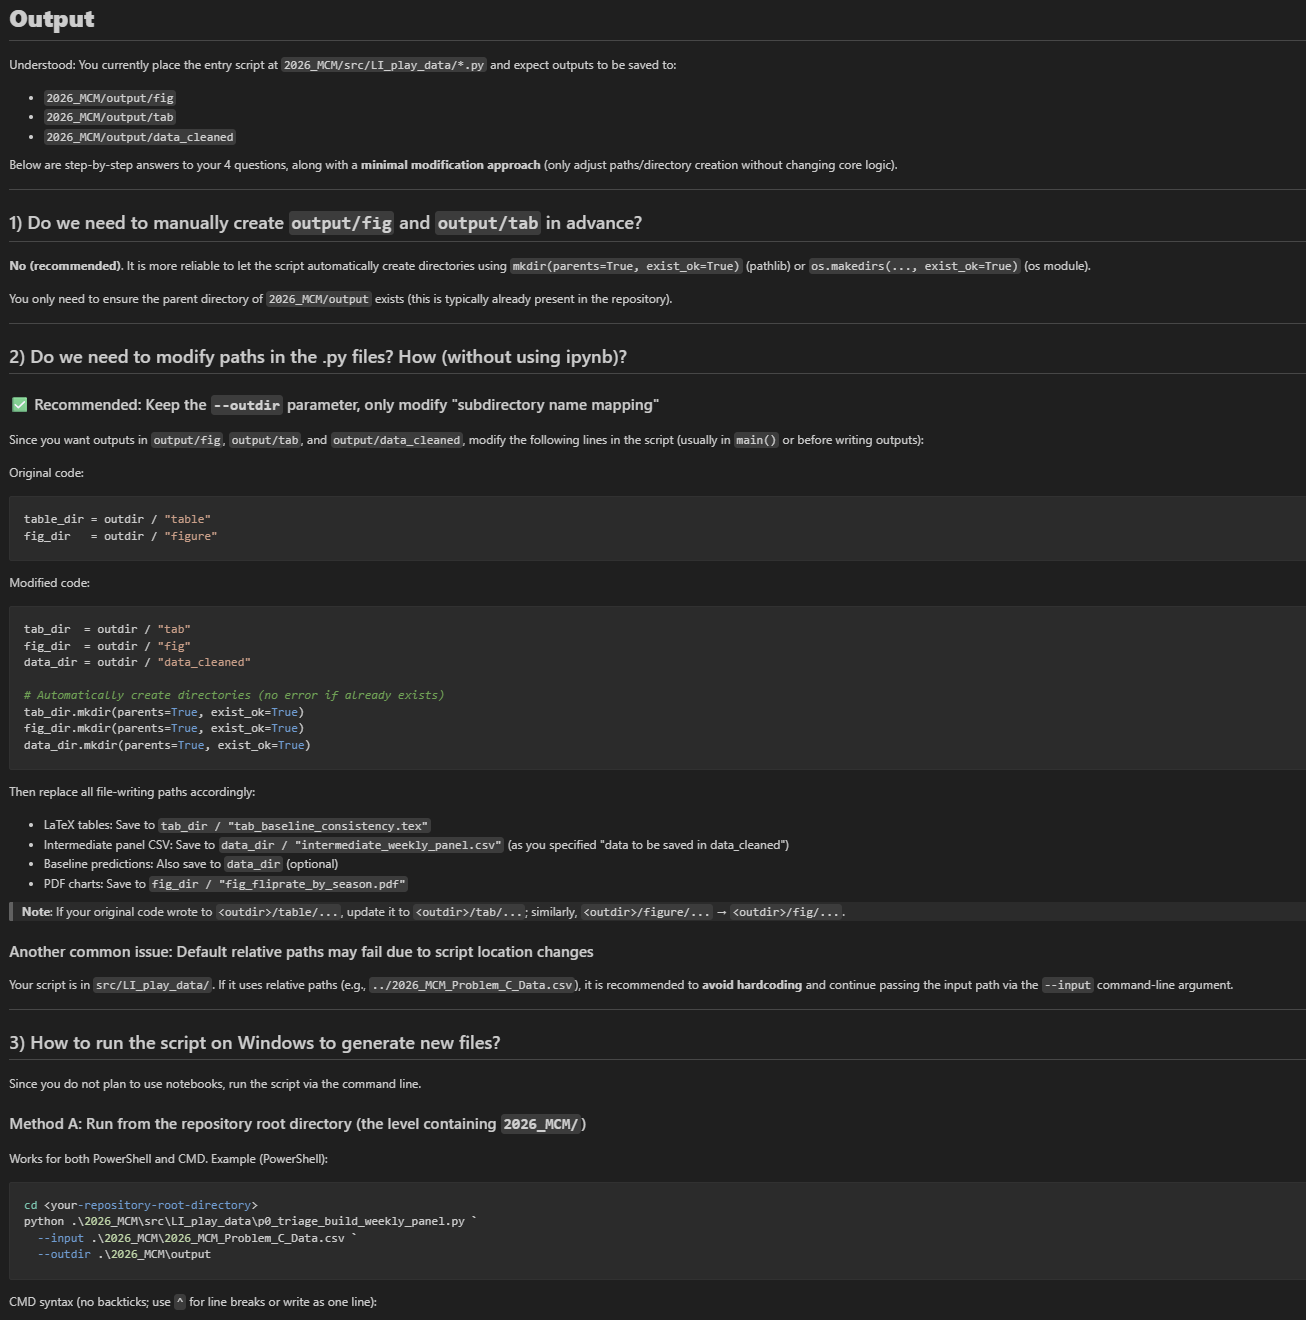
\includegraphics[width=0.9\linewidth]{report_on_use_of_ai/pho/5_1.png}
  \caption{ChatGPT Query 5 Output Screenshot}
  \label{fig:chatgpt_query_5_output}
\end{figure}
\begin{figure}[H]
  \centering
  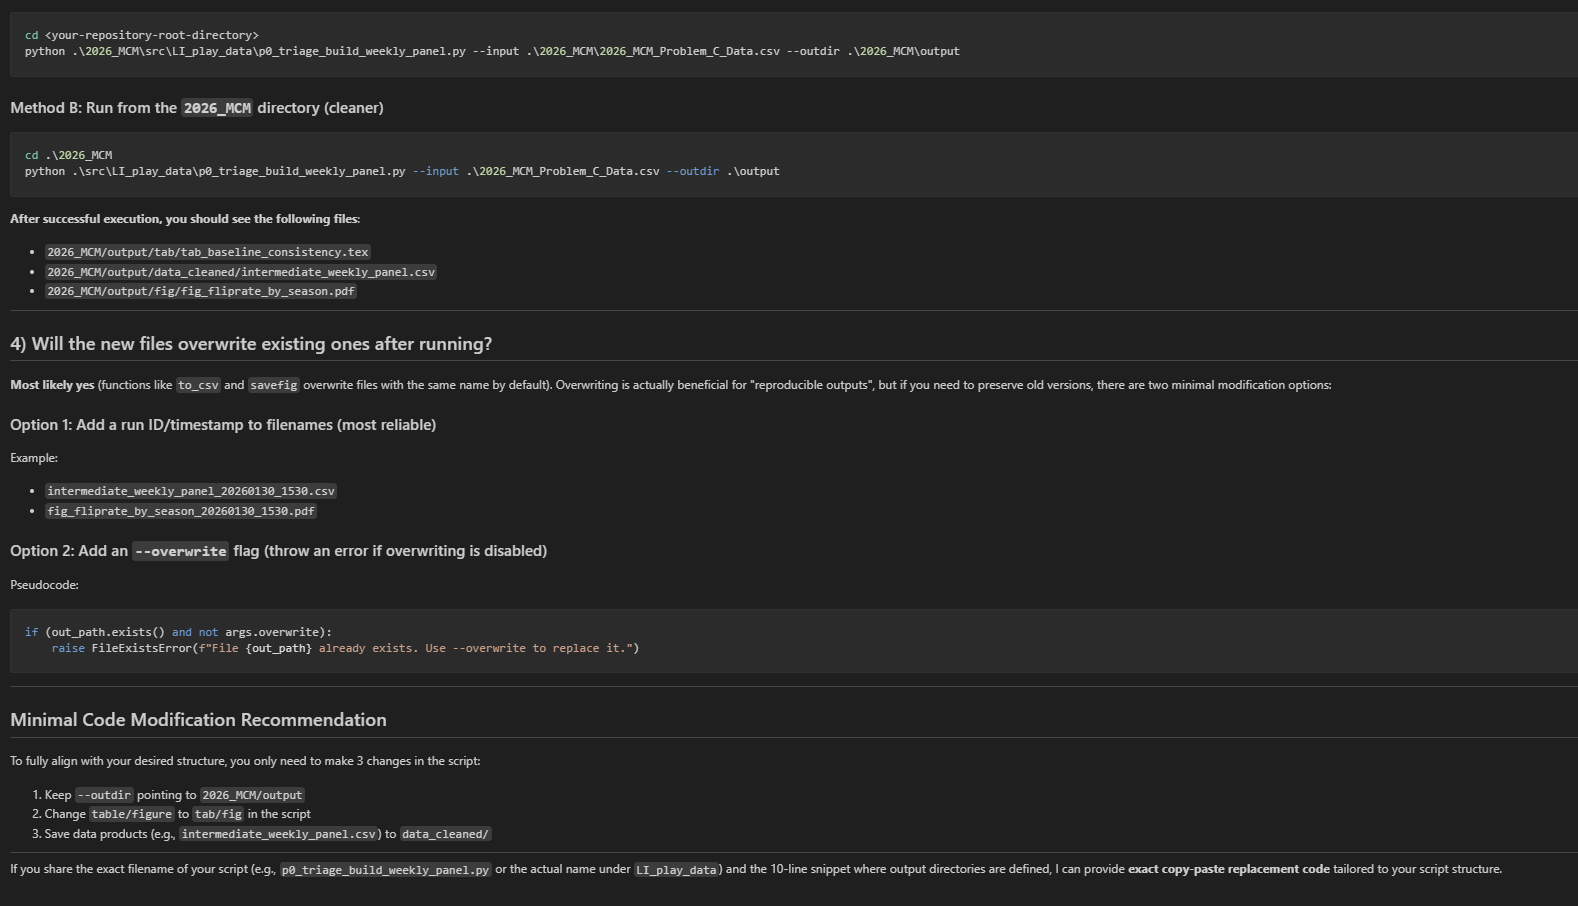
\includegraphics[width=0.9\linewidth]{report_on_use_of_ai/pho/5_2.png}
  \caption{ChatGPT Query 5 Output Screenshot}
  \label{fig:chatgpt_query_5_output_2}
\end{figure}



\textbf{\href{https://github.com/charles65536/model2026-2/blob/main/report_on_use_of_ai/chatgpt_6_input_and_output.md}{ChatGPT Query 6:}}\\
\begin{figure}[H]
  \centering
  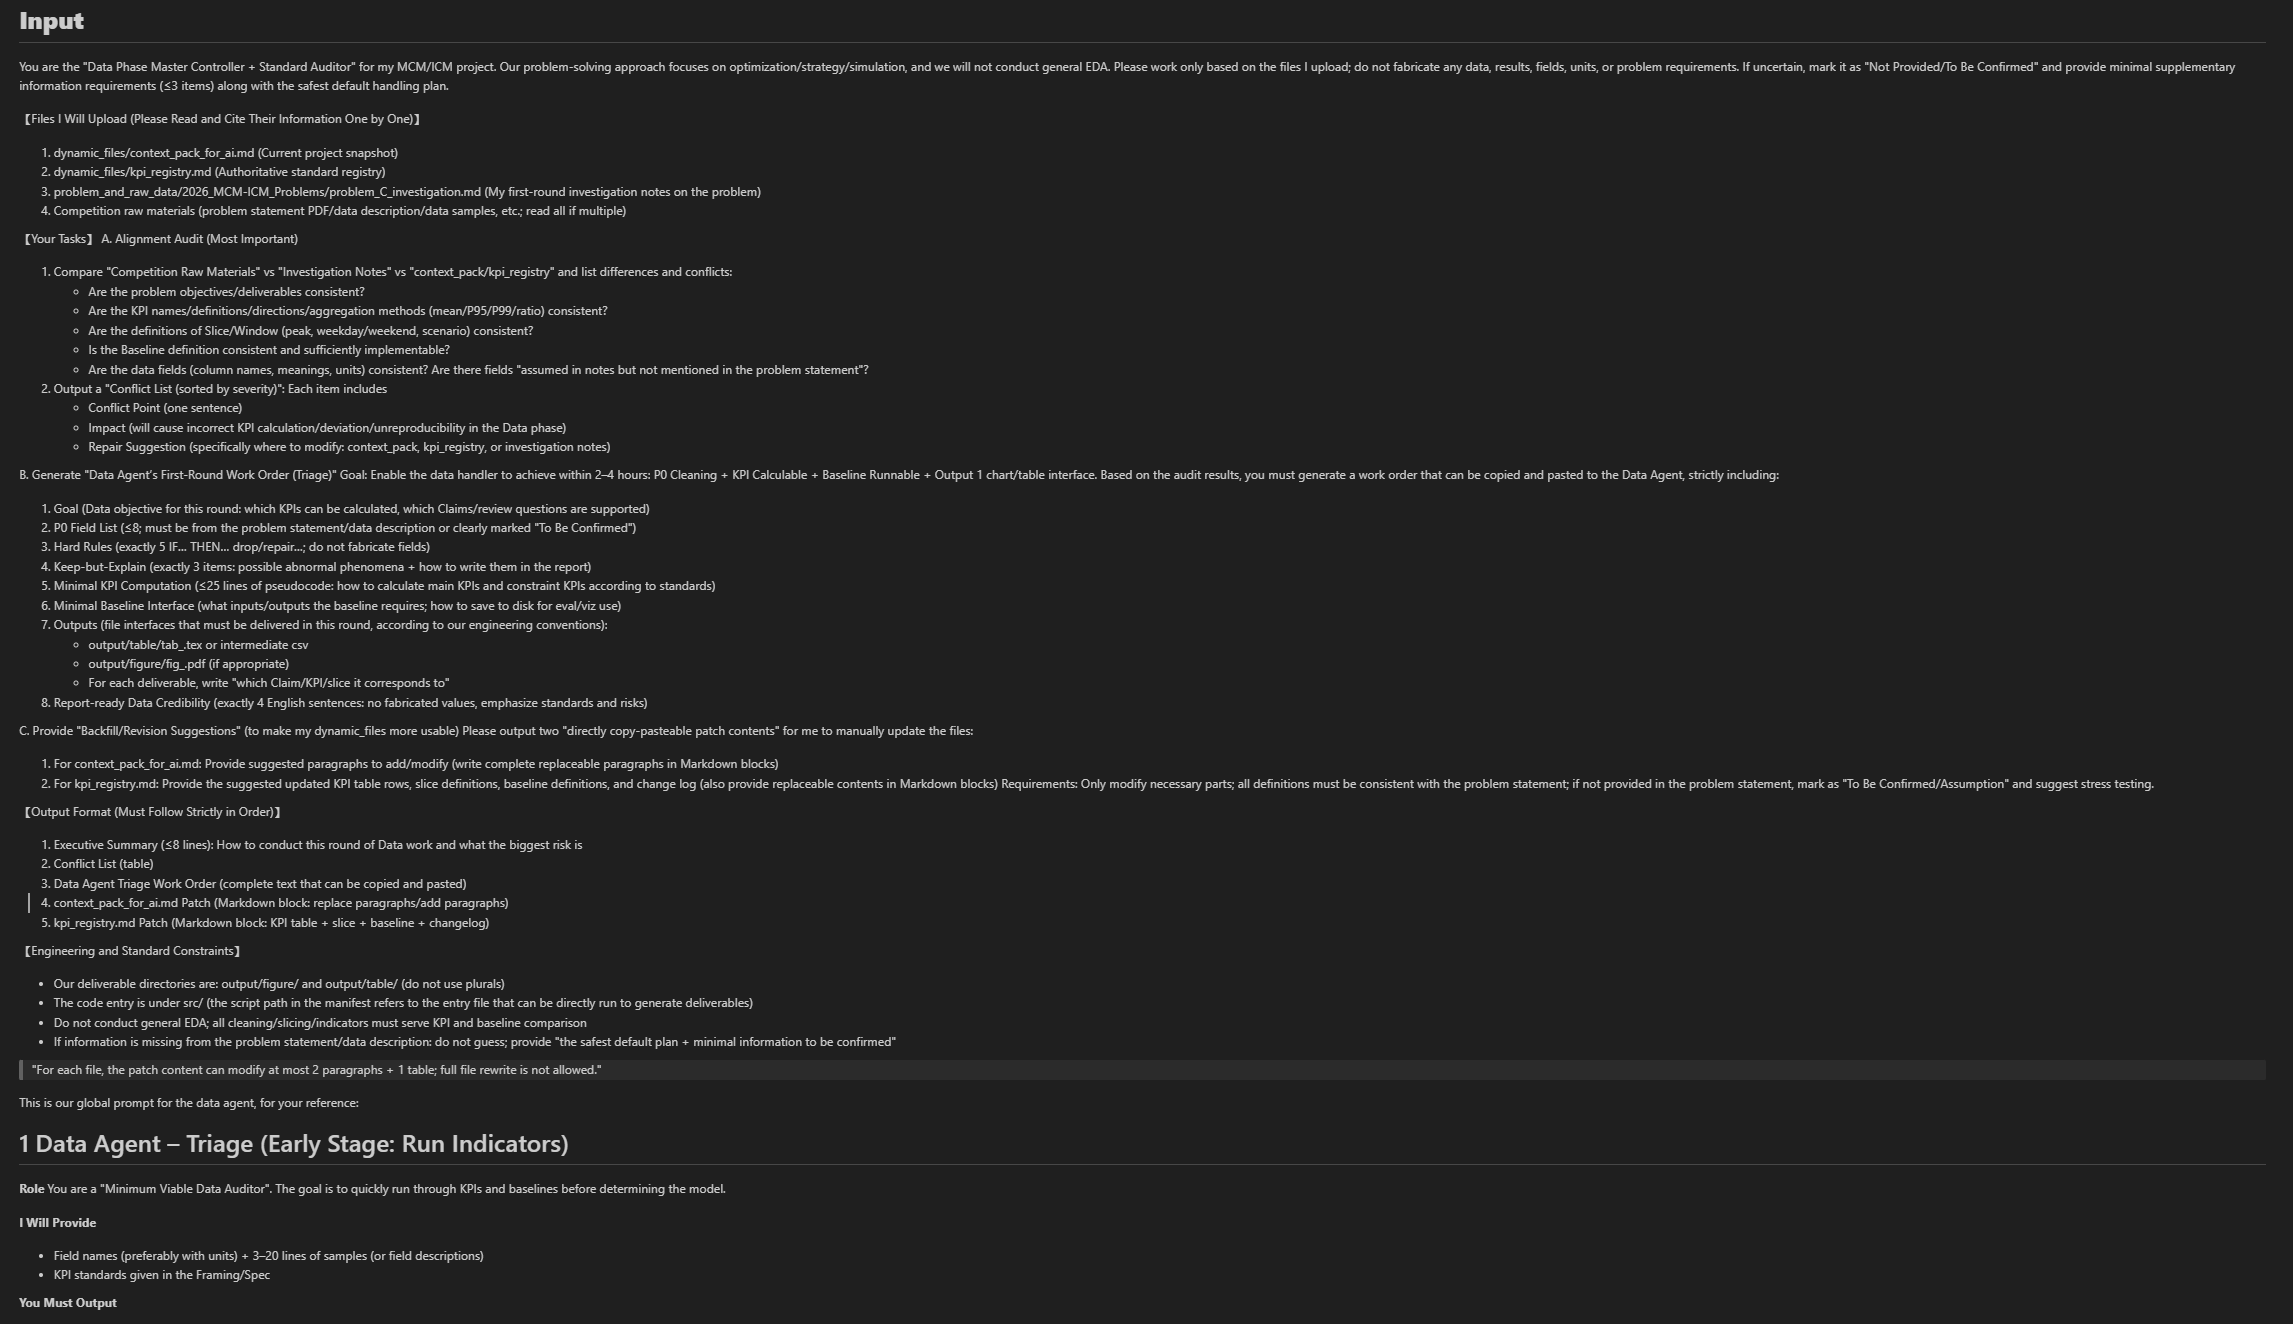
\includegraphics[width=0.9\linewidth]{report_on_use_of_ai/pho/6_1.png}
  \caption{ChatGPT Query 6 Output Screenshot}
  \label{fig:chatgpt_query_6_output}
\end{figure}
\begin{figure}[H]
  \centering
  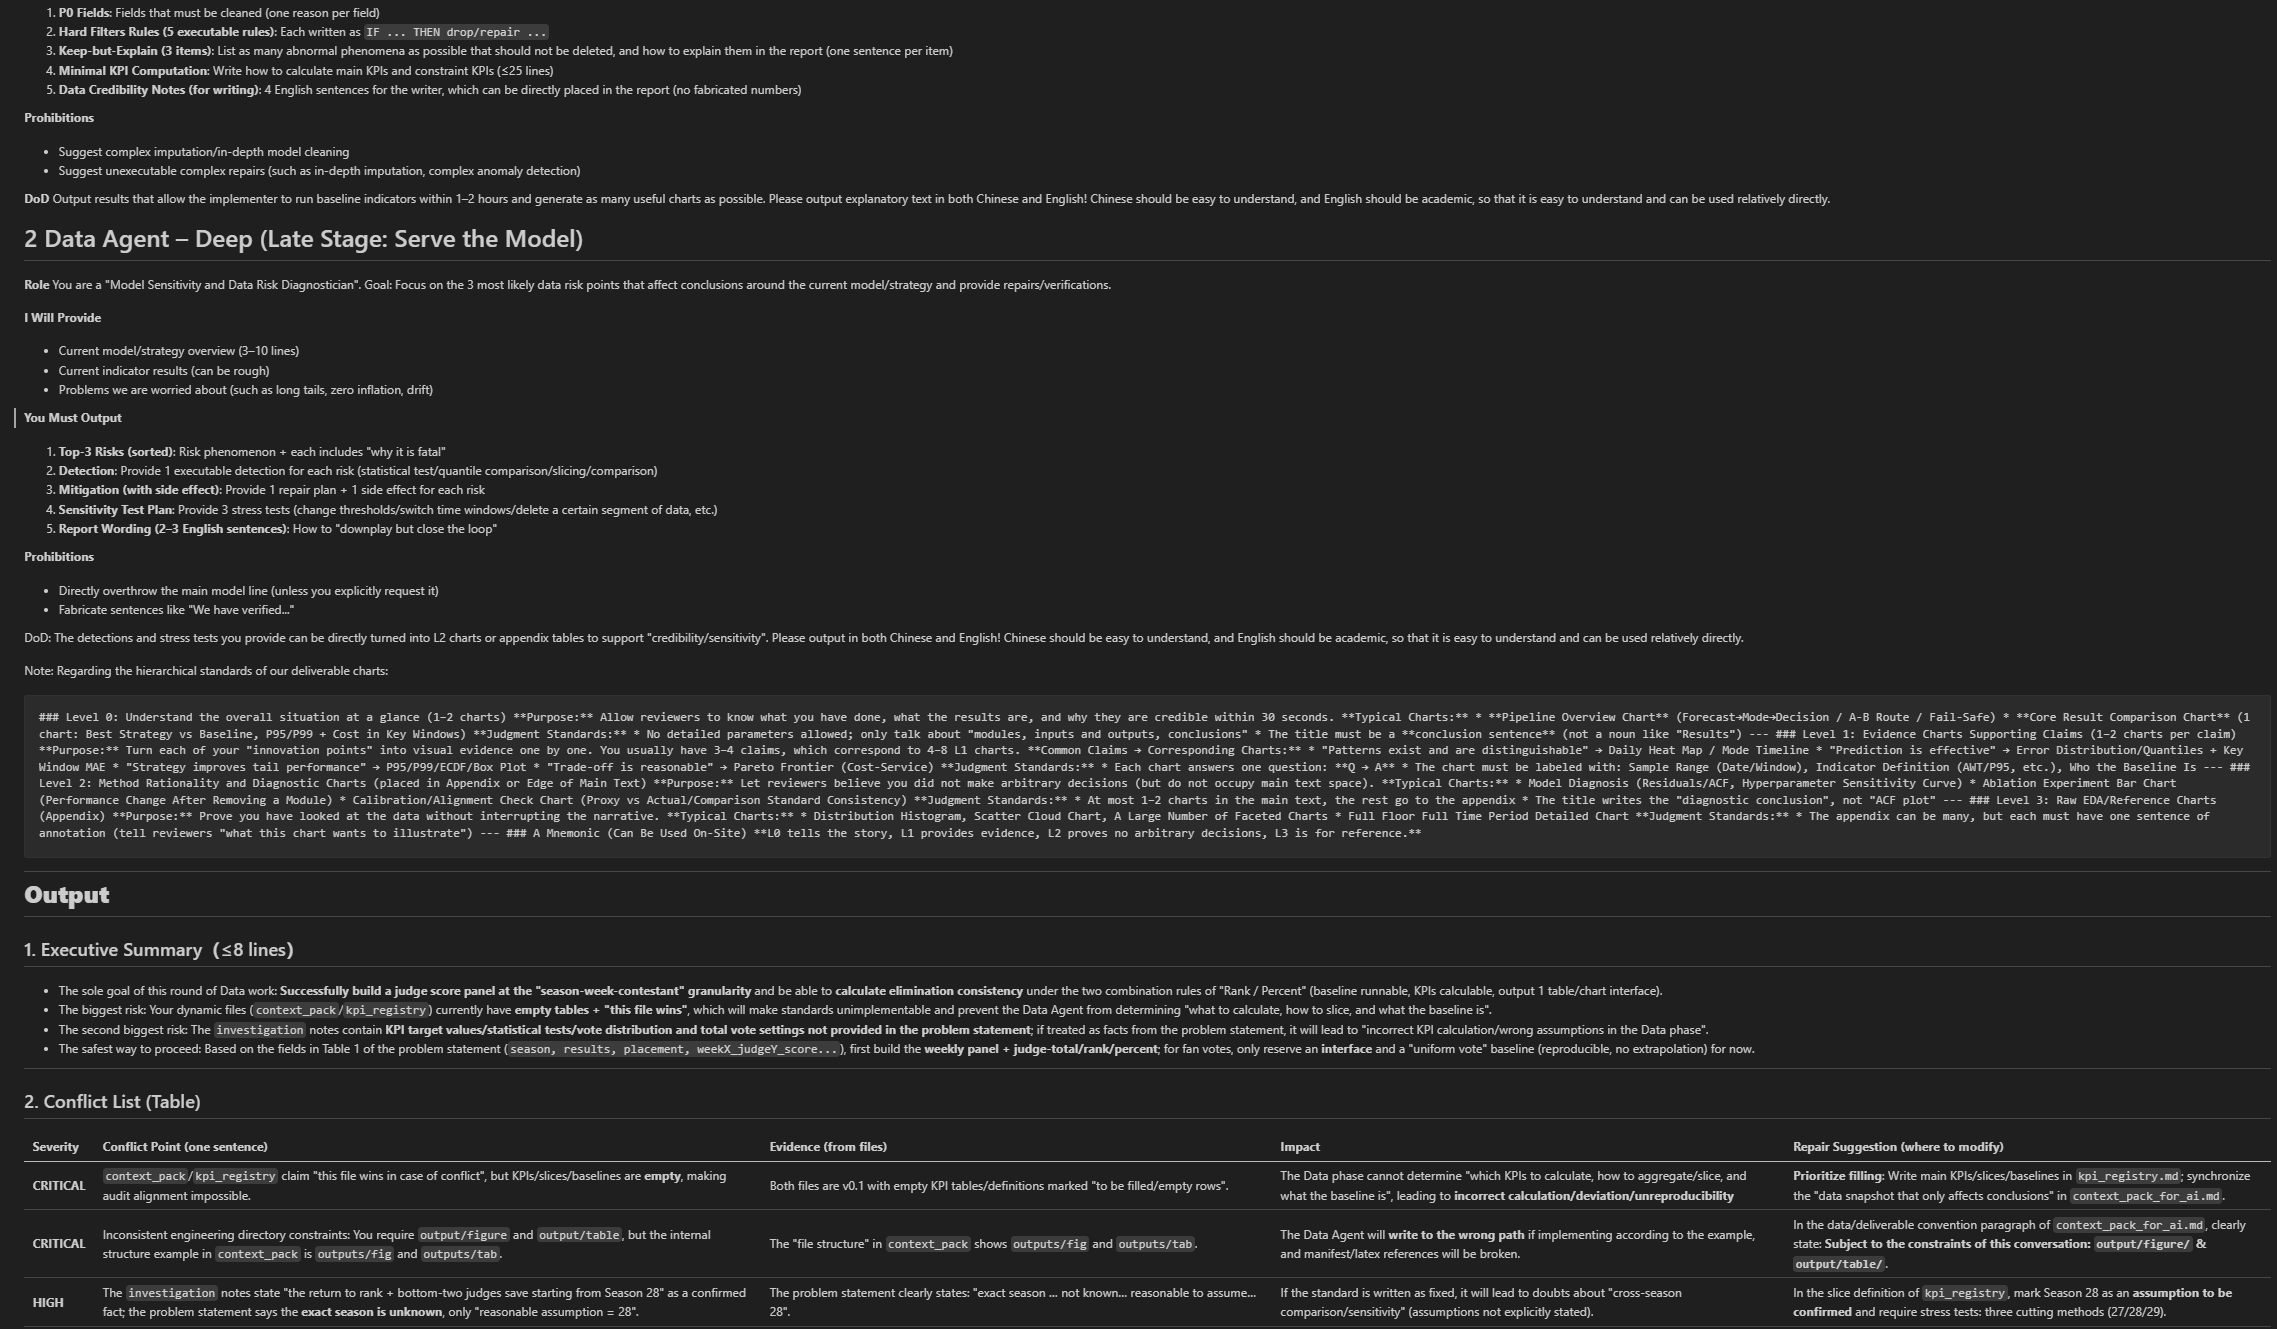
\includegraphics[width=0.9\linewidth]{report_on_use_of_ai/pho/6_2.png}
  \caption{ChatGPT Query 6 Output Screenshot}
  \label{fig:chatgpt_query_6_output2}
\end{figure}
\begin{figure}[H]
  \centering
  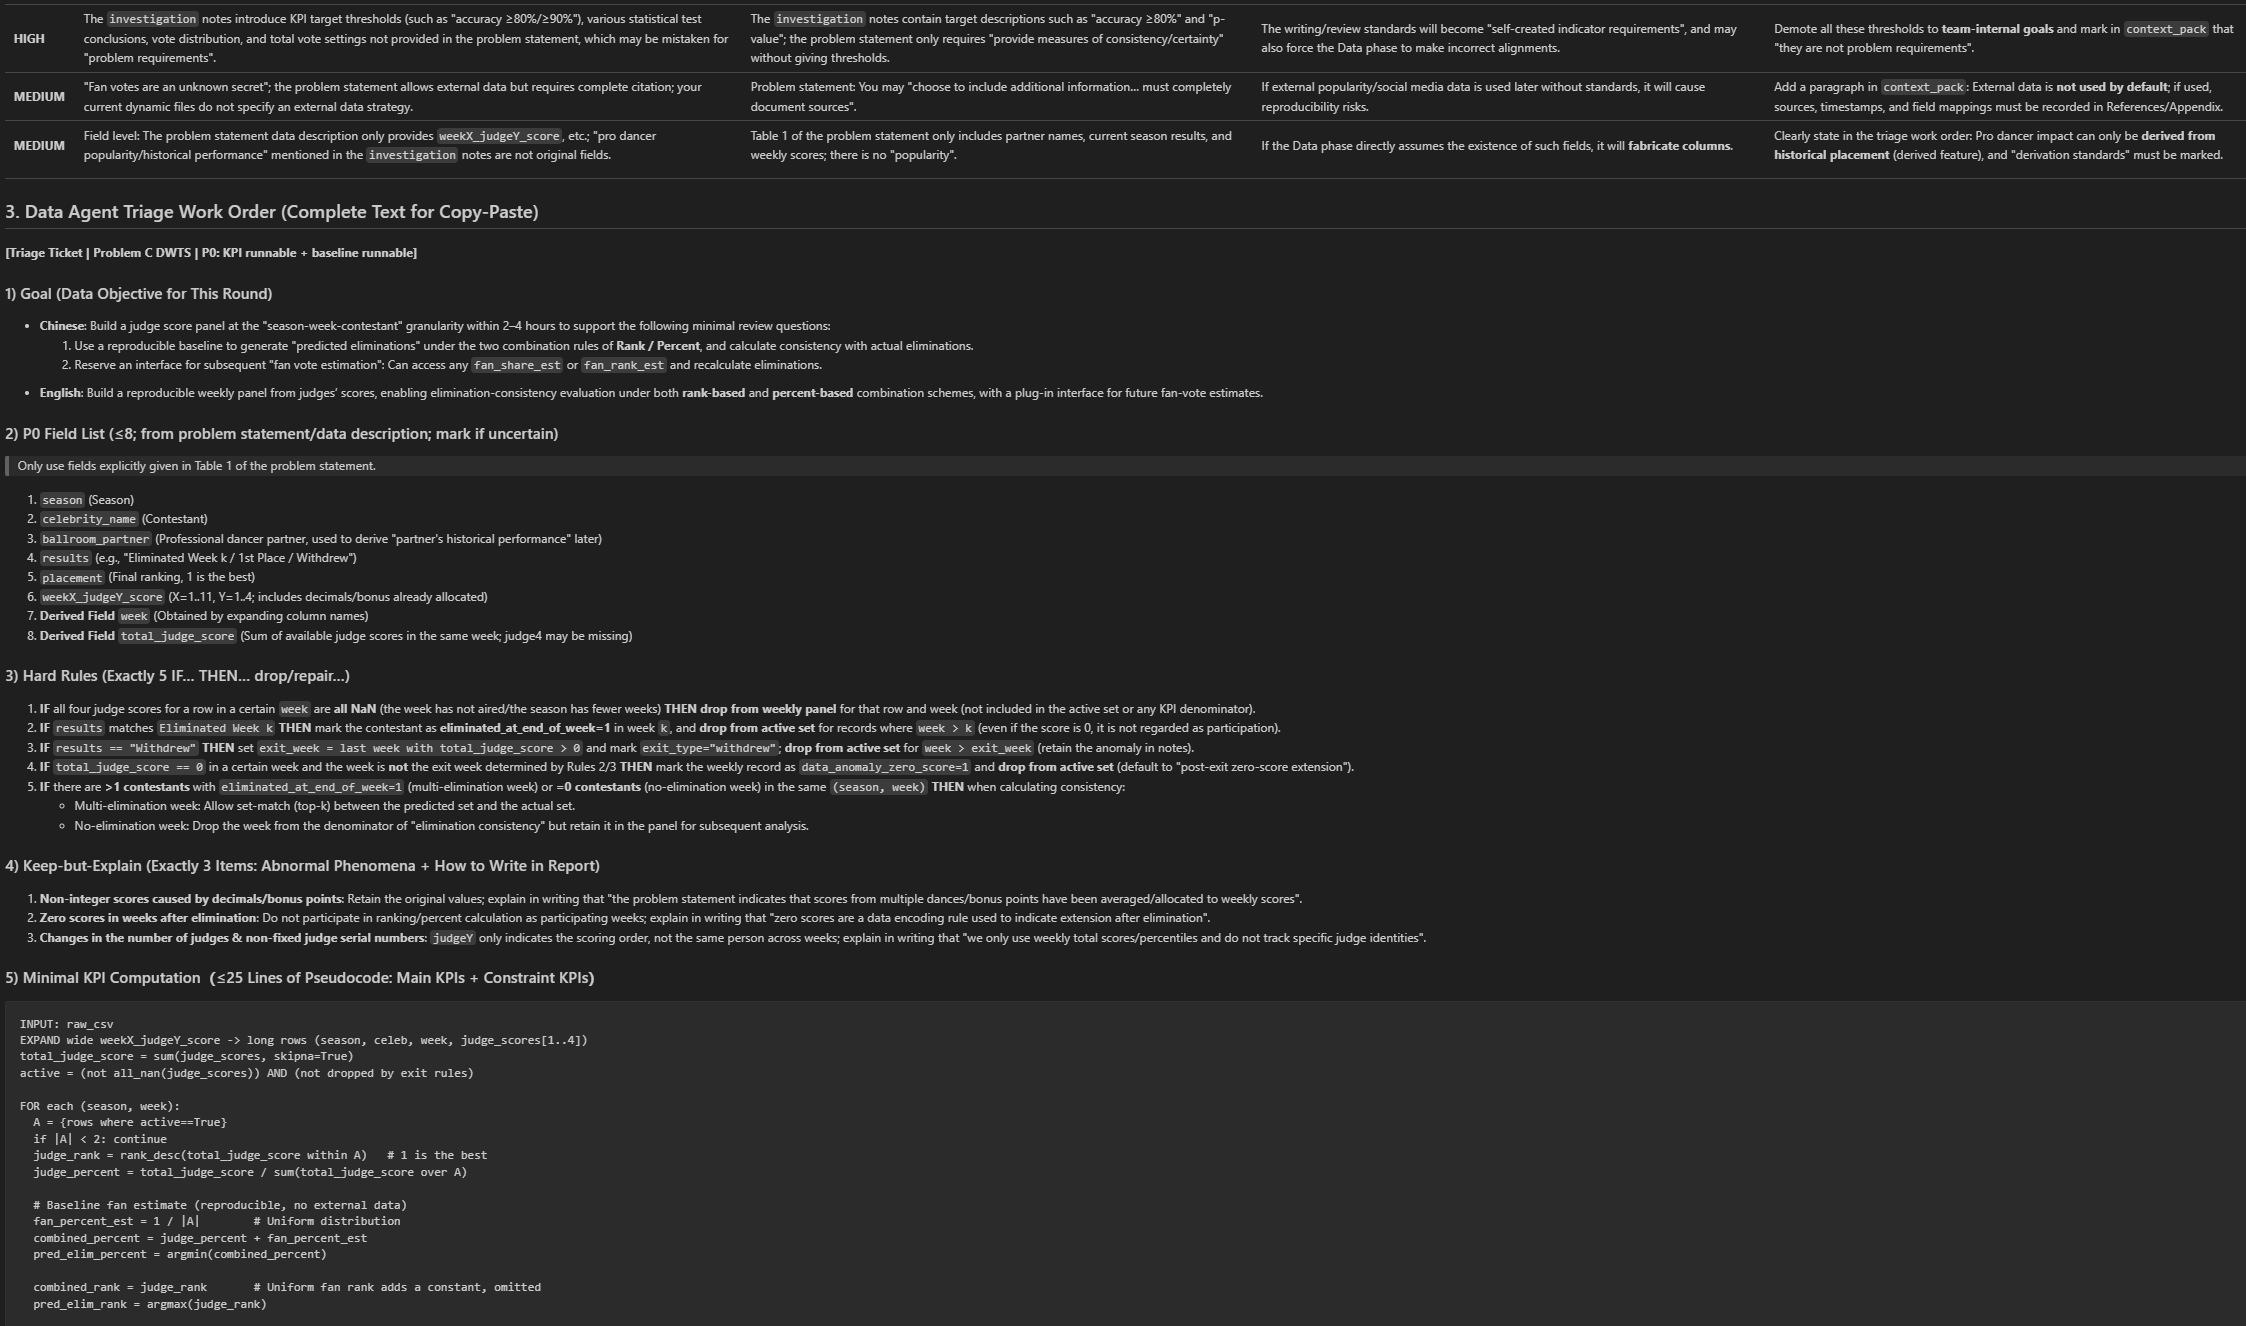
\includegraphics[width=0.9\linewidth]{report_on_use_of_ai/pho/6_3.png}
  \caption{ChatGPT Query 6 Output Screenshot}
  \label{fig:chatgpt_query_6_output3}
\end{figure}
\begin{figure}[H]
  \centering
  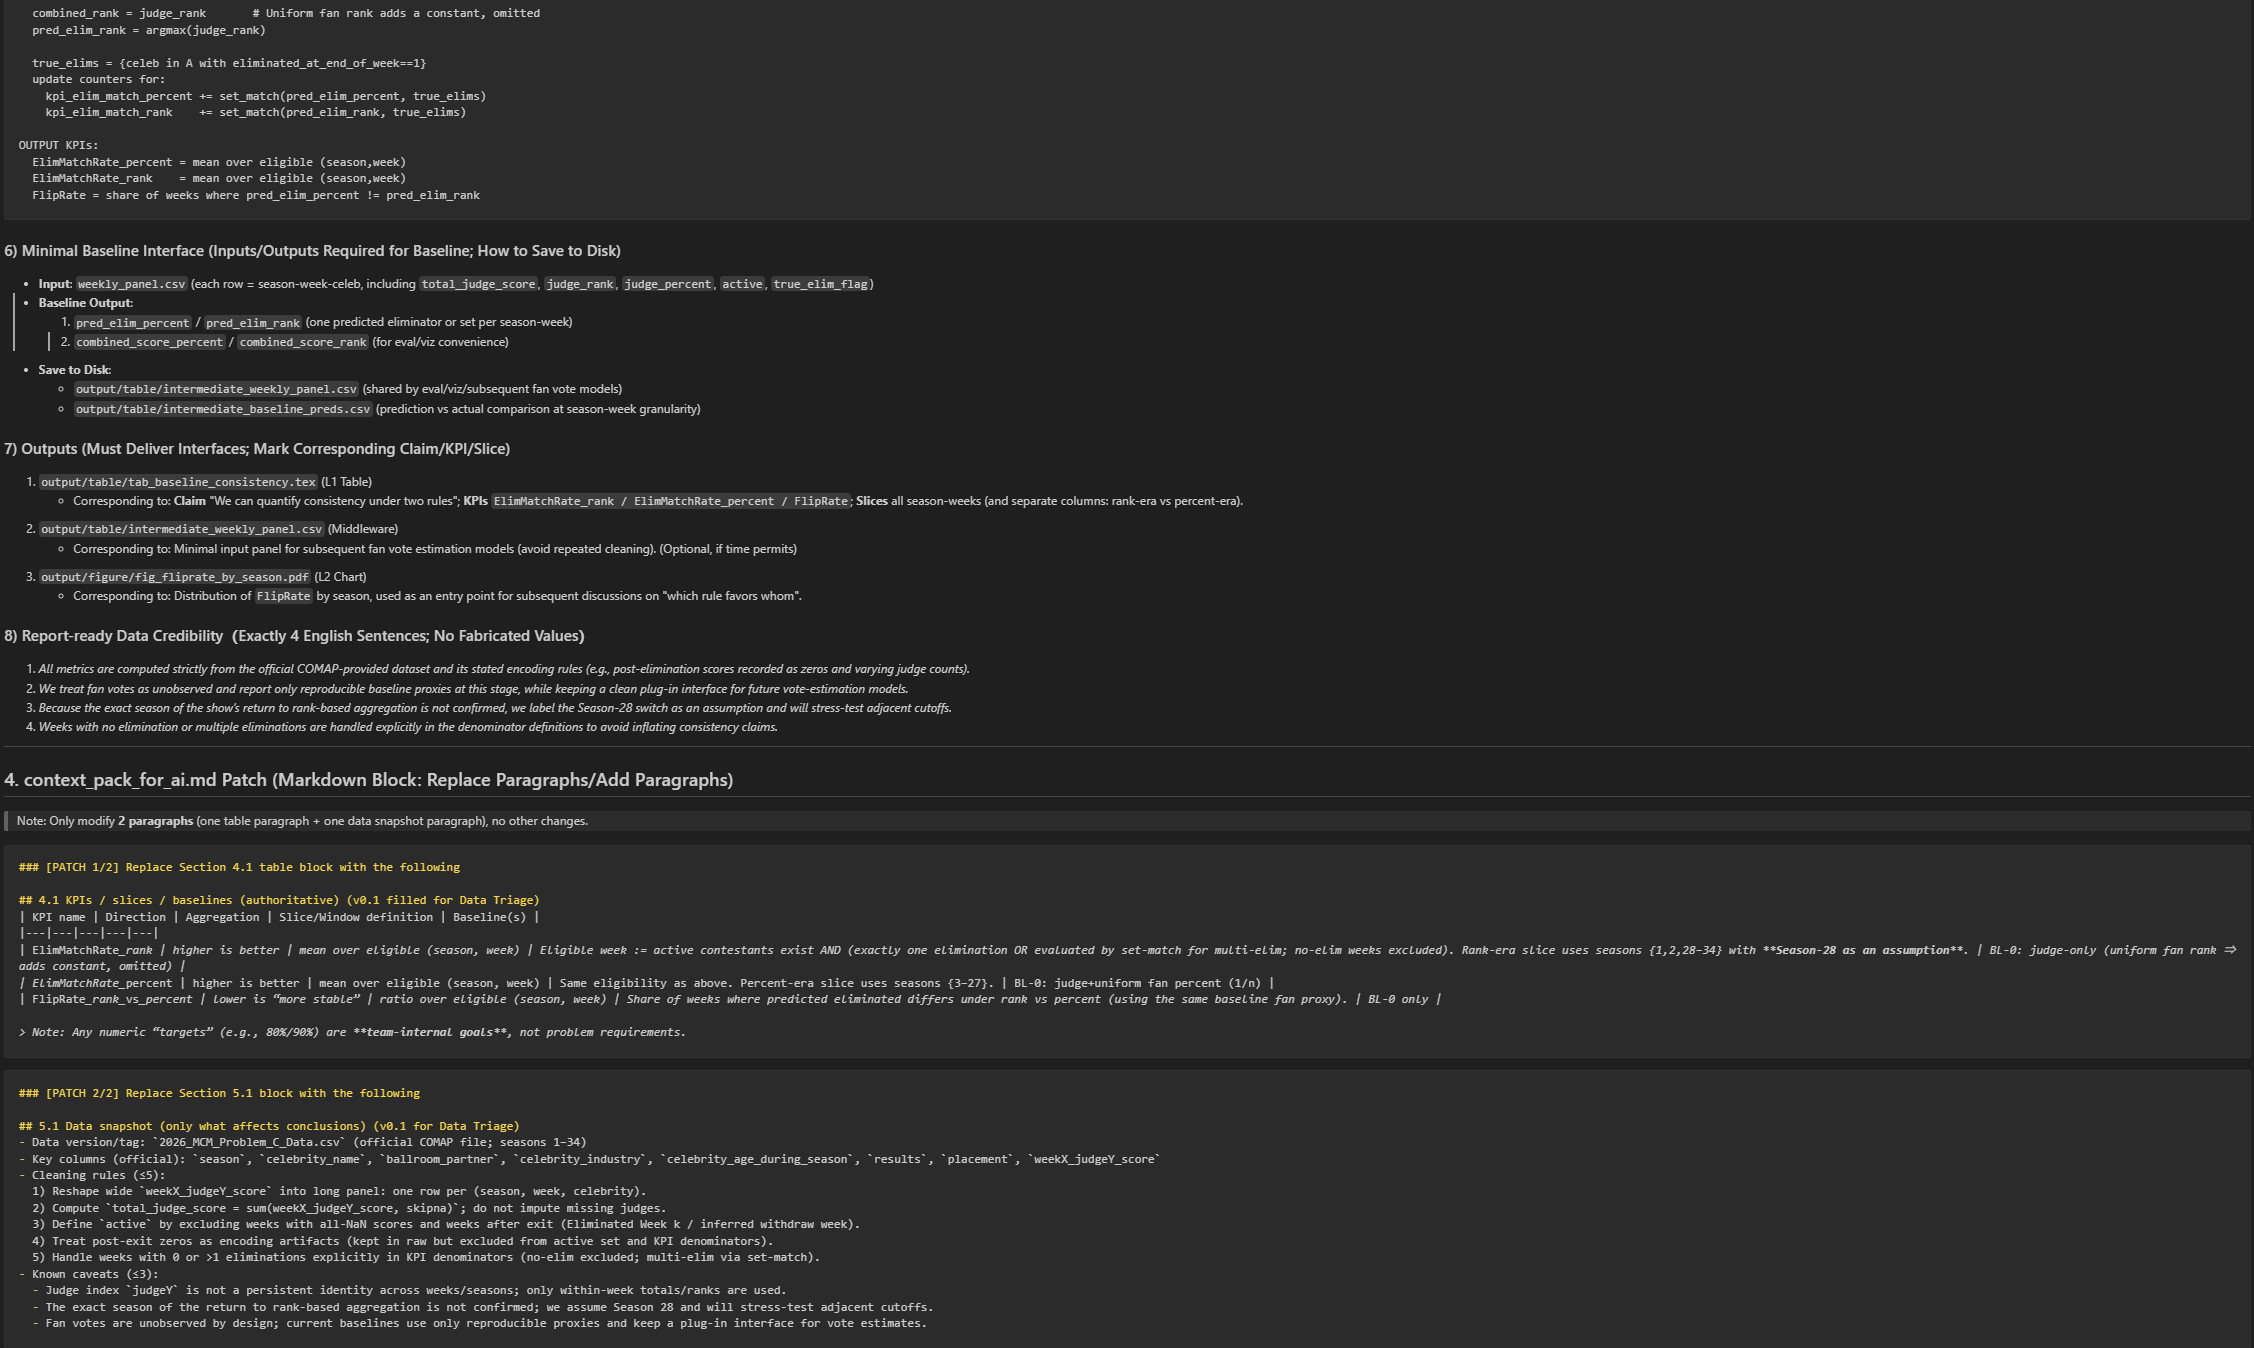
\includegraphics[width=0.9\linewidth]{report_on_use_of_ai/pho/6_4.png}
  \caption{ChatGPT Query 6 Output Screenshot}
  \label{fig:chatgpt_query_6_output4}
\end{figure}
\begin{figure}[H]
  \centering
  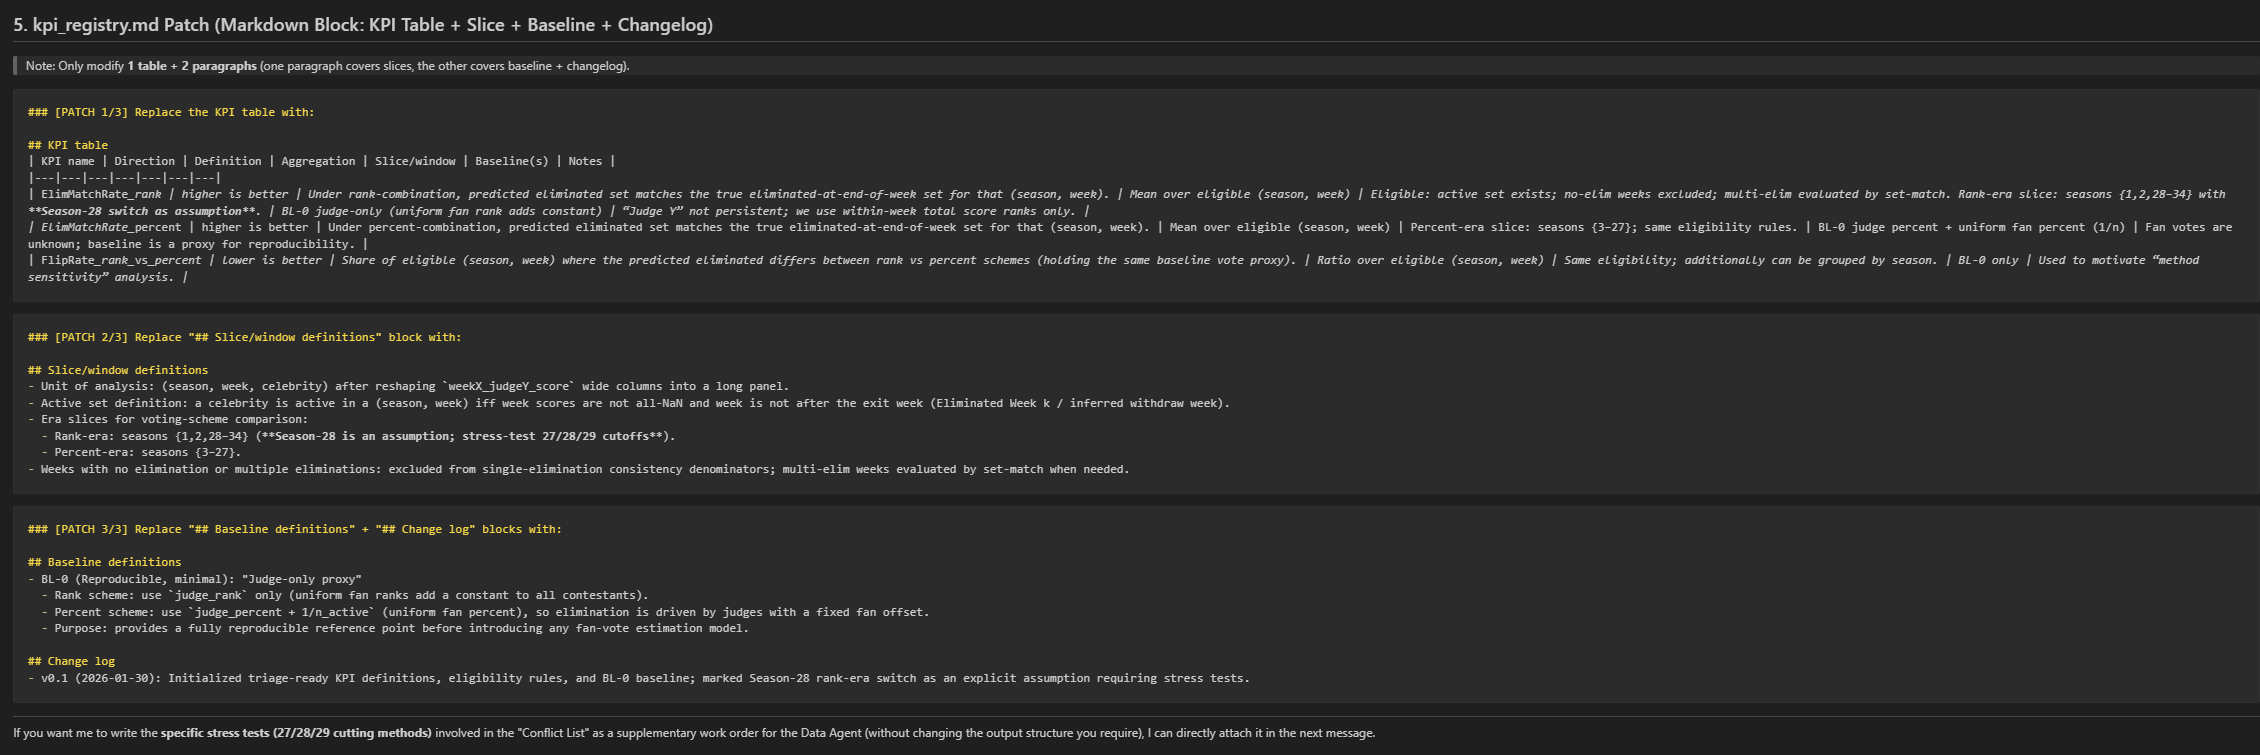
\includegraphics[width=0.9\linewidth]{report_on_use_of_ai/pho/6_5.png}
  \caption{ChatGPT Query 6 Output Screenshot}
  \label{fig:chatgpt_query_6_output5}
\end{figure}


\textbf{\href{https://github.com/charles65536/model2026-2/blob/main/report_on_use_of_ai/chatgpt_7_input_and_output.md}{ChatGPT Query 7:}}\\
\textbf{Input:}
What should we do regarding the previous conversation? Because the investigation file is non-authoritative; the files we feed to the agent do not include the investigation—it is only used for us to check if our framing/spec agent has any important omissions. Now clearly tell me how to use the information you provided above (e.g., 3. Place the Data Agent Triage work order in... file / place it separately in the conversation as a prompt).\\
\textbf{Output:}
\begin{figure}[H]
  \centering
  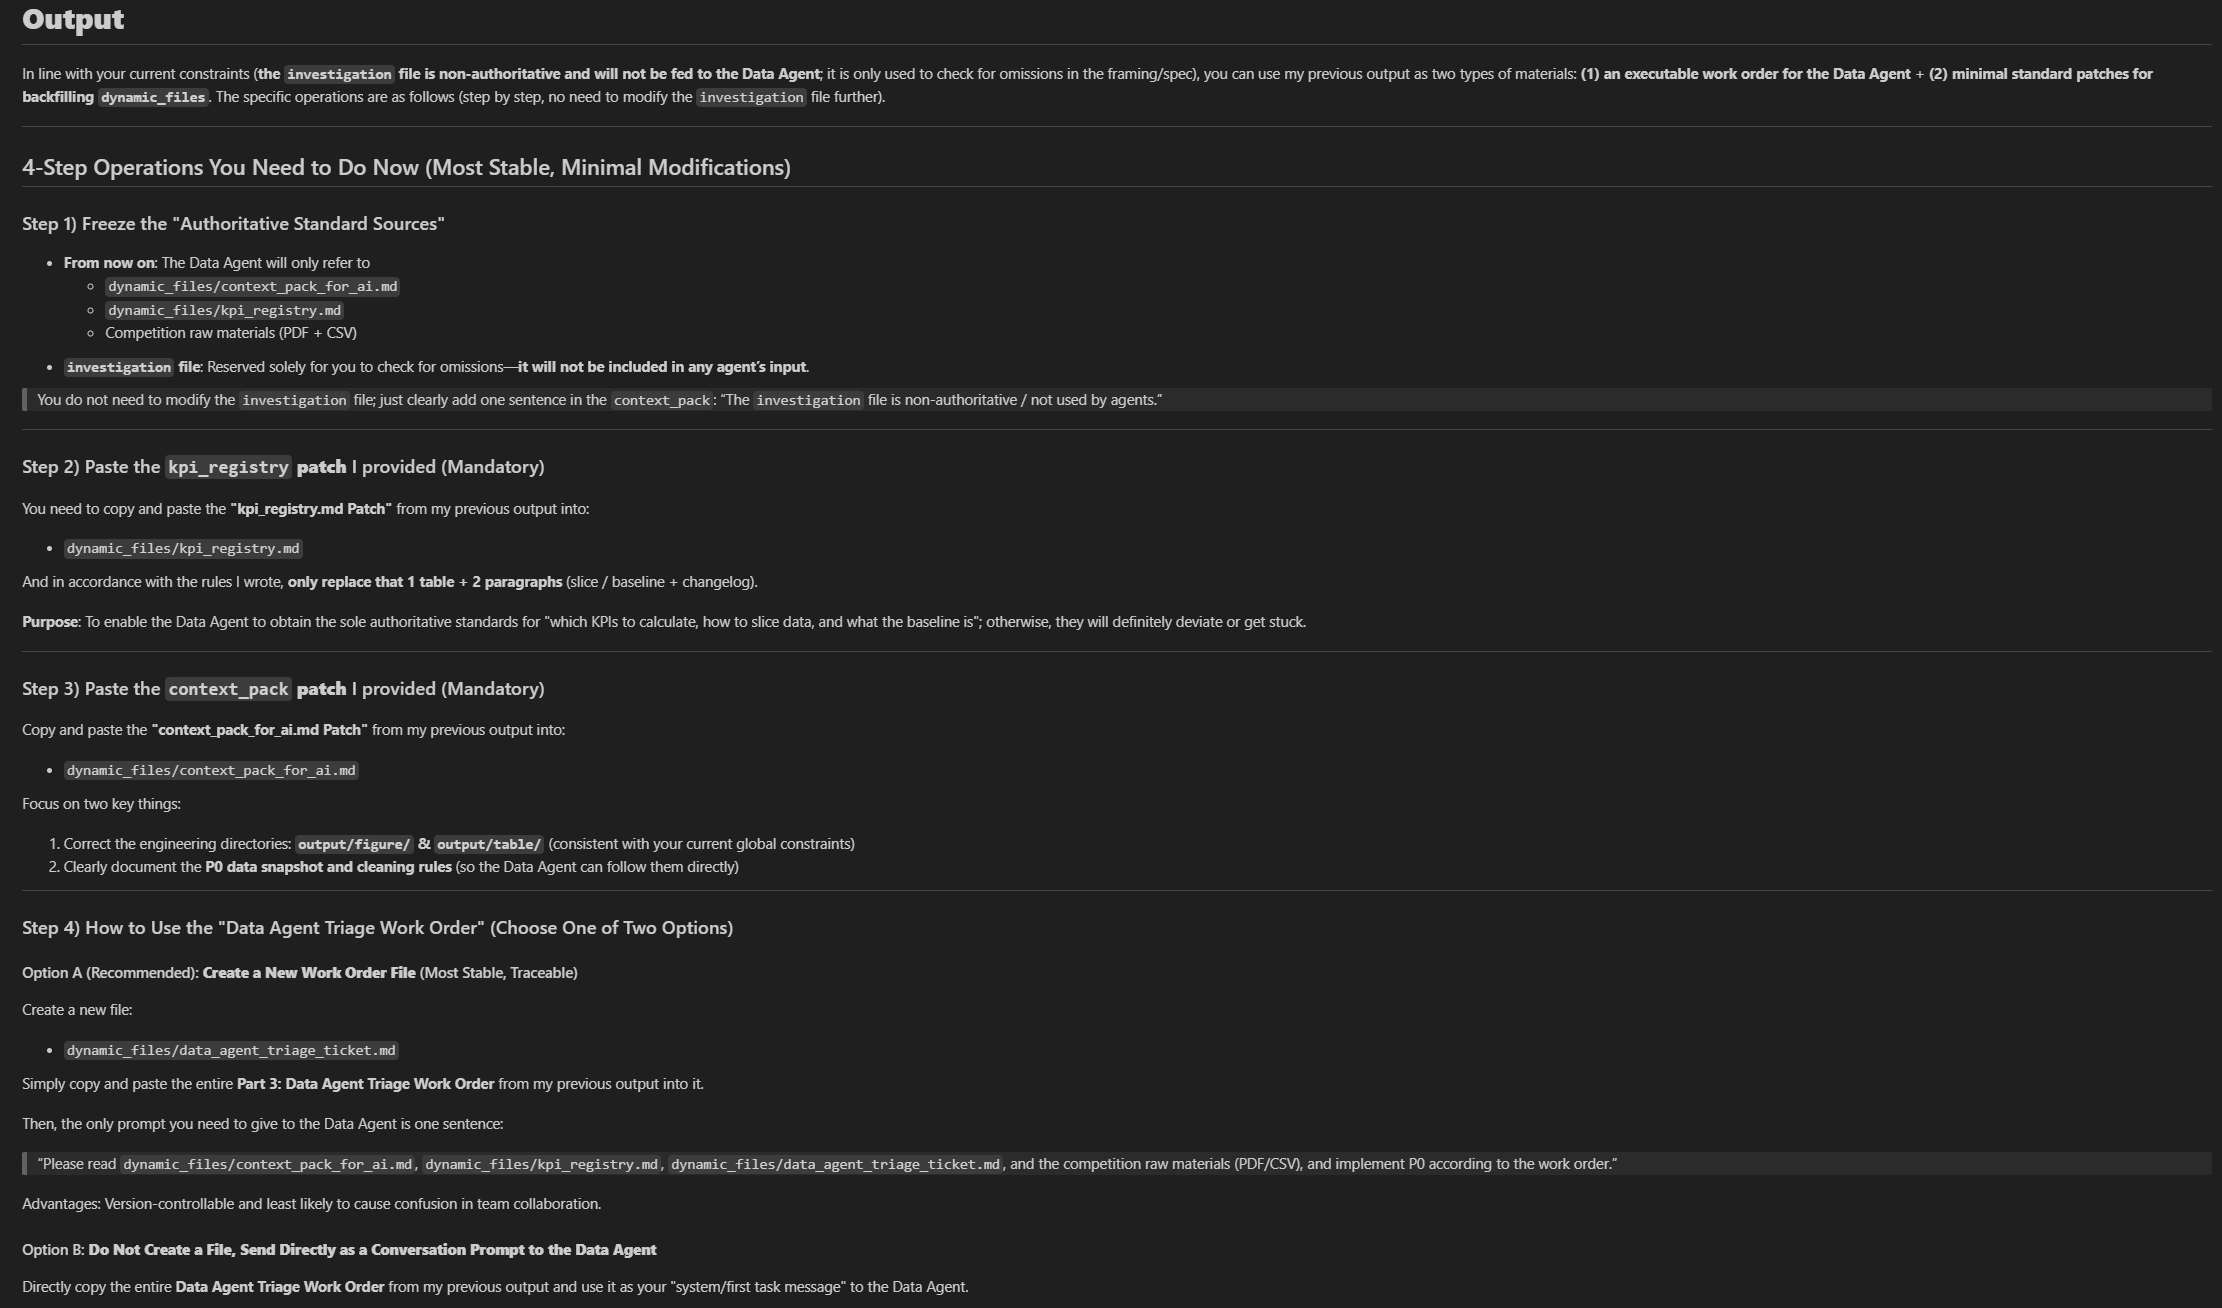
\includegraphics[width=0.9\linewidth]{report_on_use_of_ai/pho/7_1.png}
  \caption{ChatGPT Query 7 Output Screenshot}
  \label{fig:chatgpt_query_7_output}
\end{figure}
\begin{figure}[H]
  \centering
  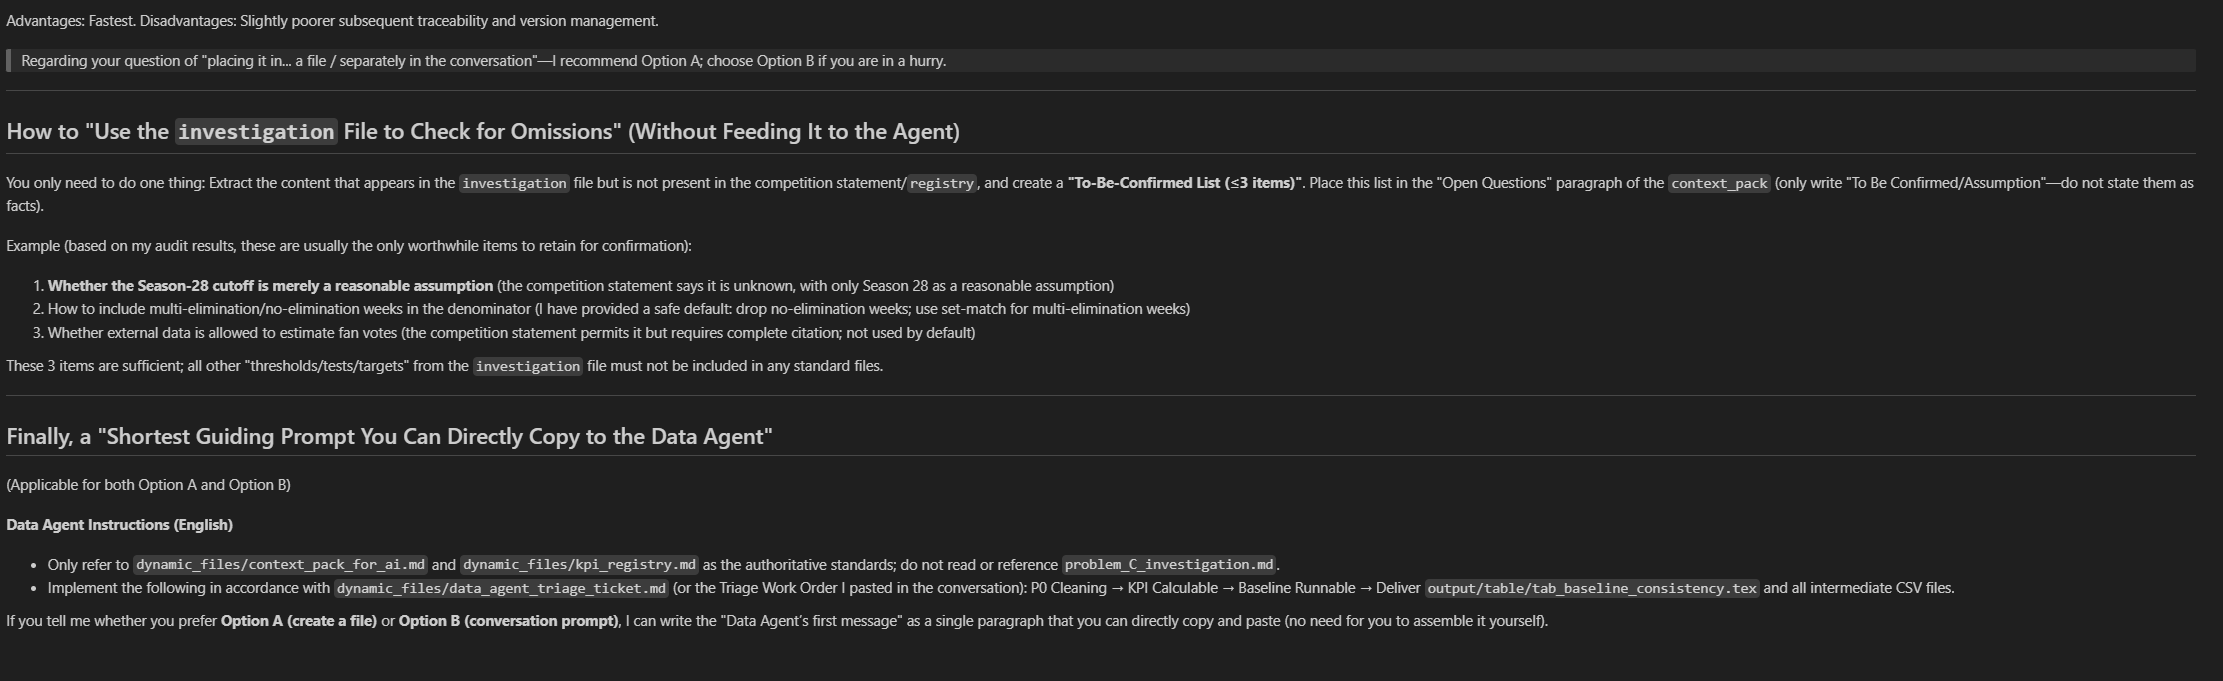
\includegraphics[width=0.9\linewidth]{report_on_use_of_ai/pho/7_2.png}
  \caption{ChatGPT Query 7 Output Screenshot}
  \label{fig:chatgpt_query_7_output2}
\end{figure}

\textbf{\href{https://github.com/charles65536/model2026-2/blob/main/report_on_use_of_ai/chatgpt_8_input_and_output.md}{ChatGPT Query 8:}}\\
\textbf{Input:}
'Handling of "Withdrew": Should it be "exclude after inferring the exit week" or "exclude the entire season from the consistency denominator"?
Consistency denominator: Exclude no-elimination weeks, use set-match for multi-elimination weeks (is this acceptable?).'
What is the best way to handle this? Is it part of our cleaning standards? If we only add this one-sentence patch, will it cause huge problems in subsequent data processing?\\
\textbf{Output:}
\begin{figure}[H]
  \centering
  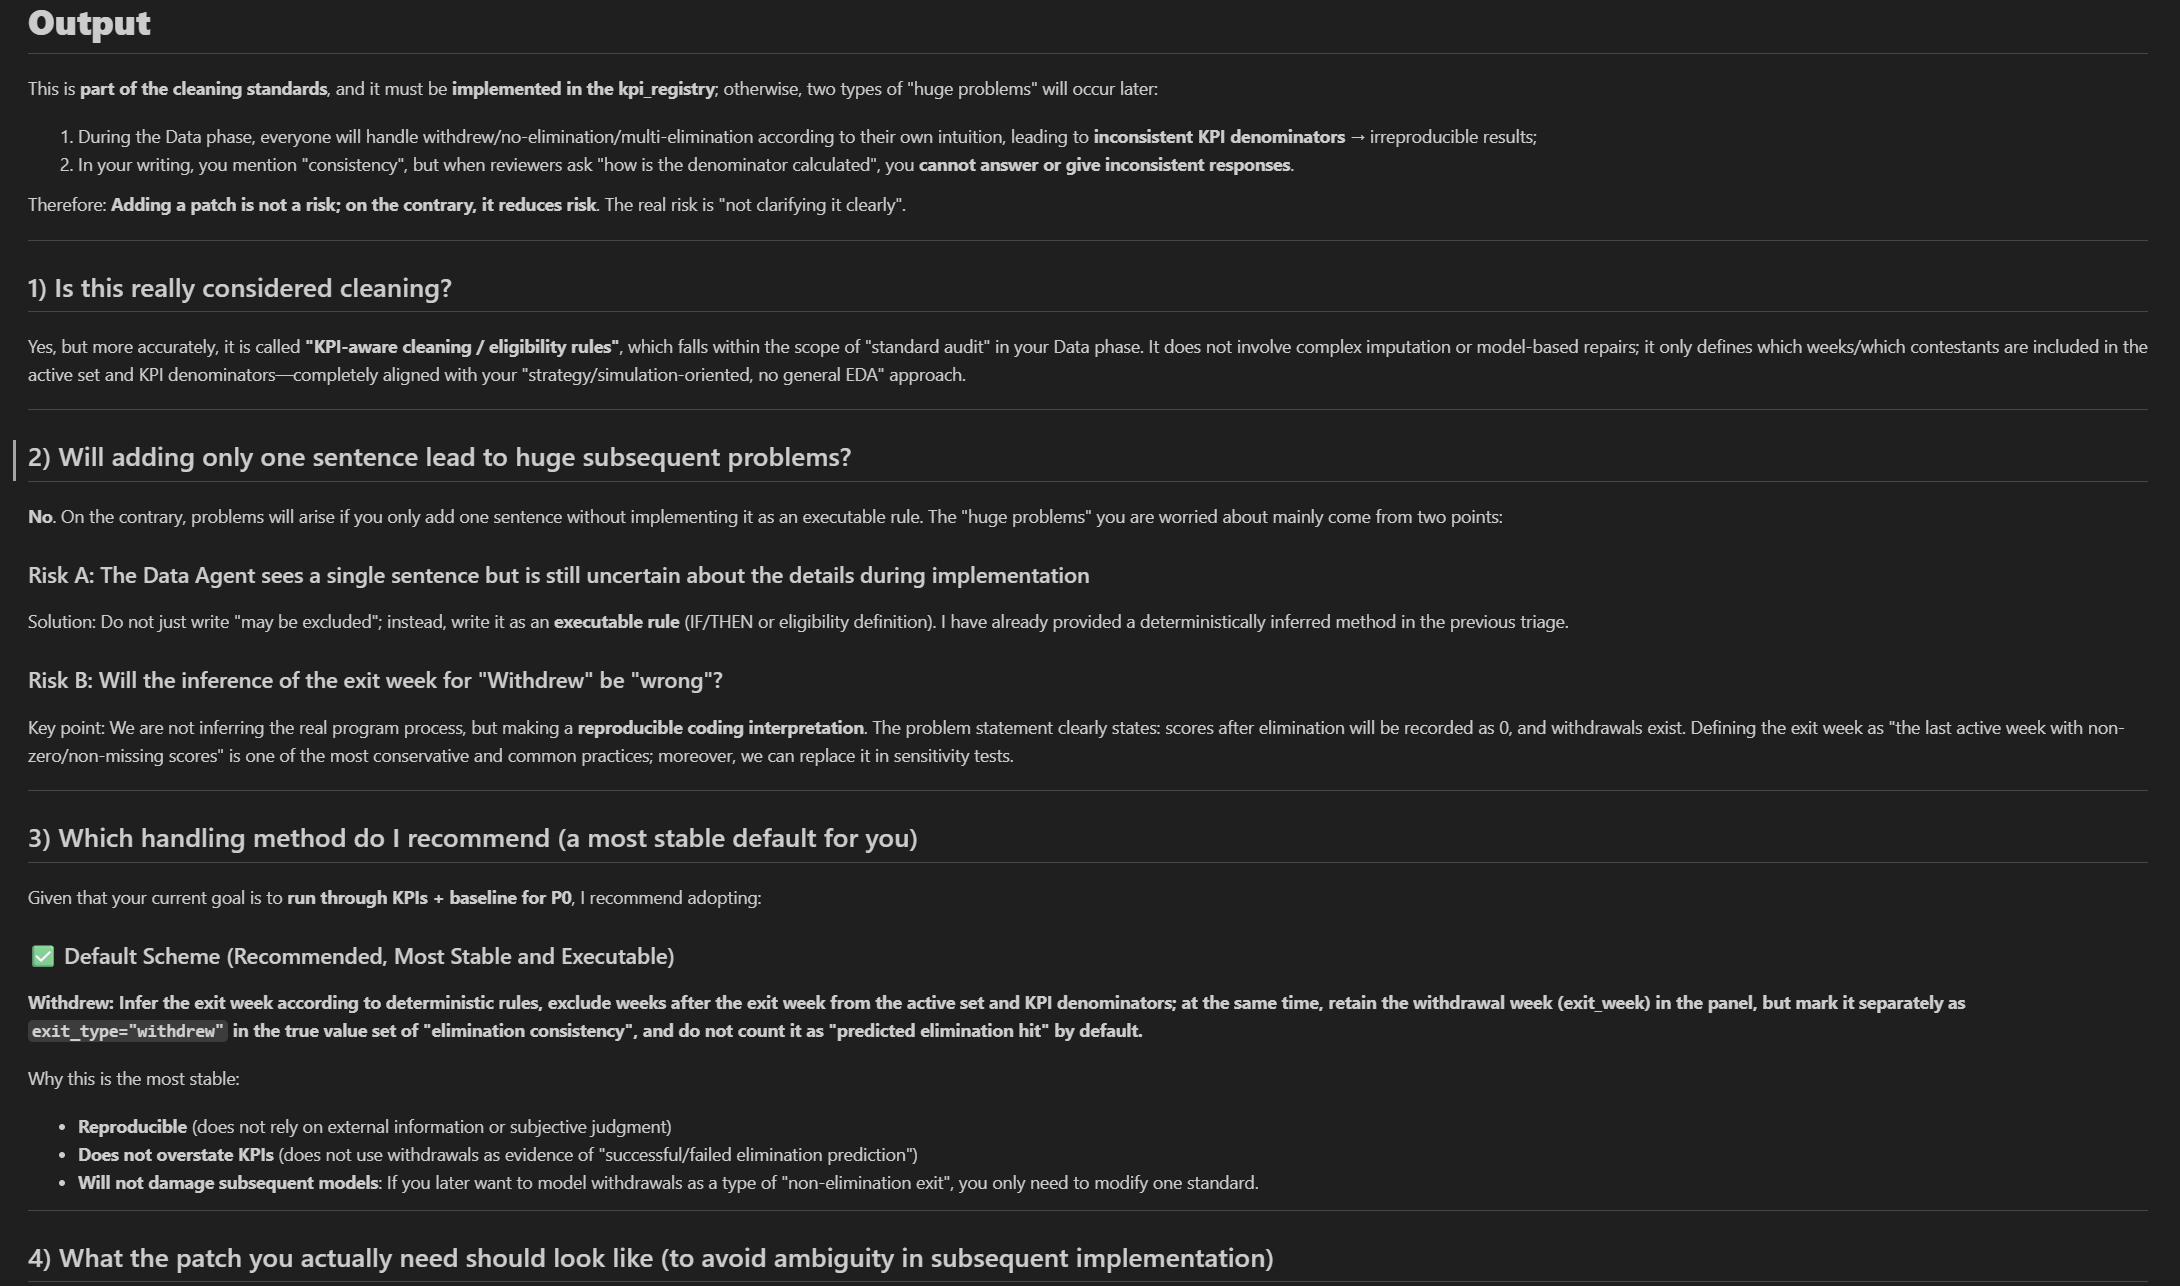
\includegraphics[width=0.9\linewidth]{report_on_use_of_ai/pho/81.png}
  \caption{ChatGPT Query 8 Output Screenshot}
  \label{fig:chatgpt_query_8_output}
\end{figure}
\begin{figure}[H]
  \centering
  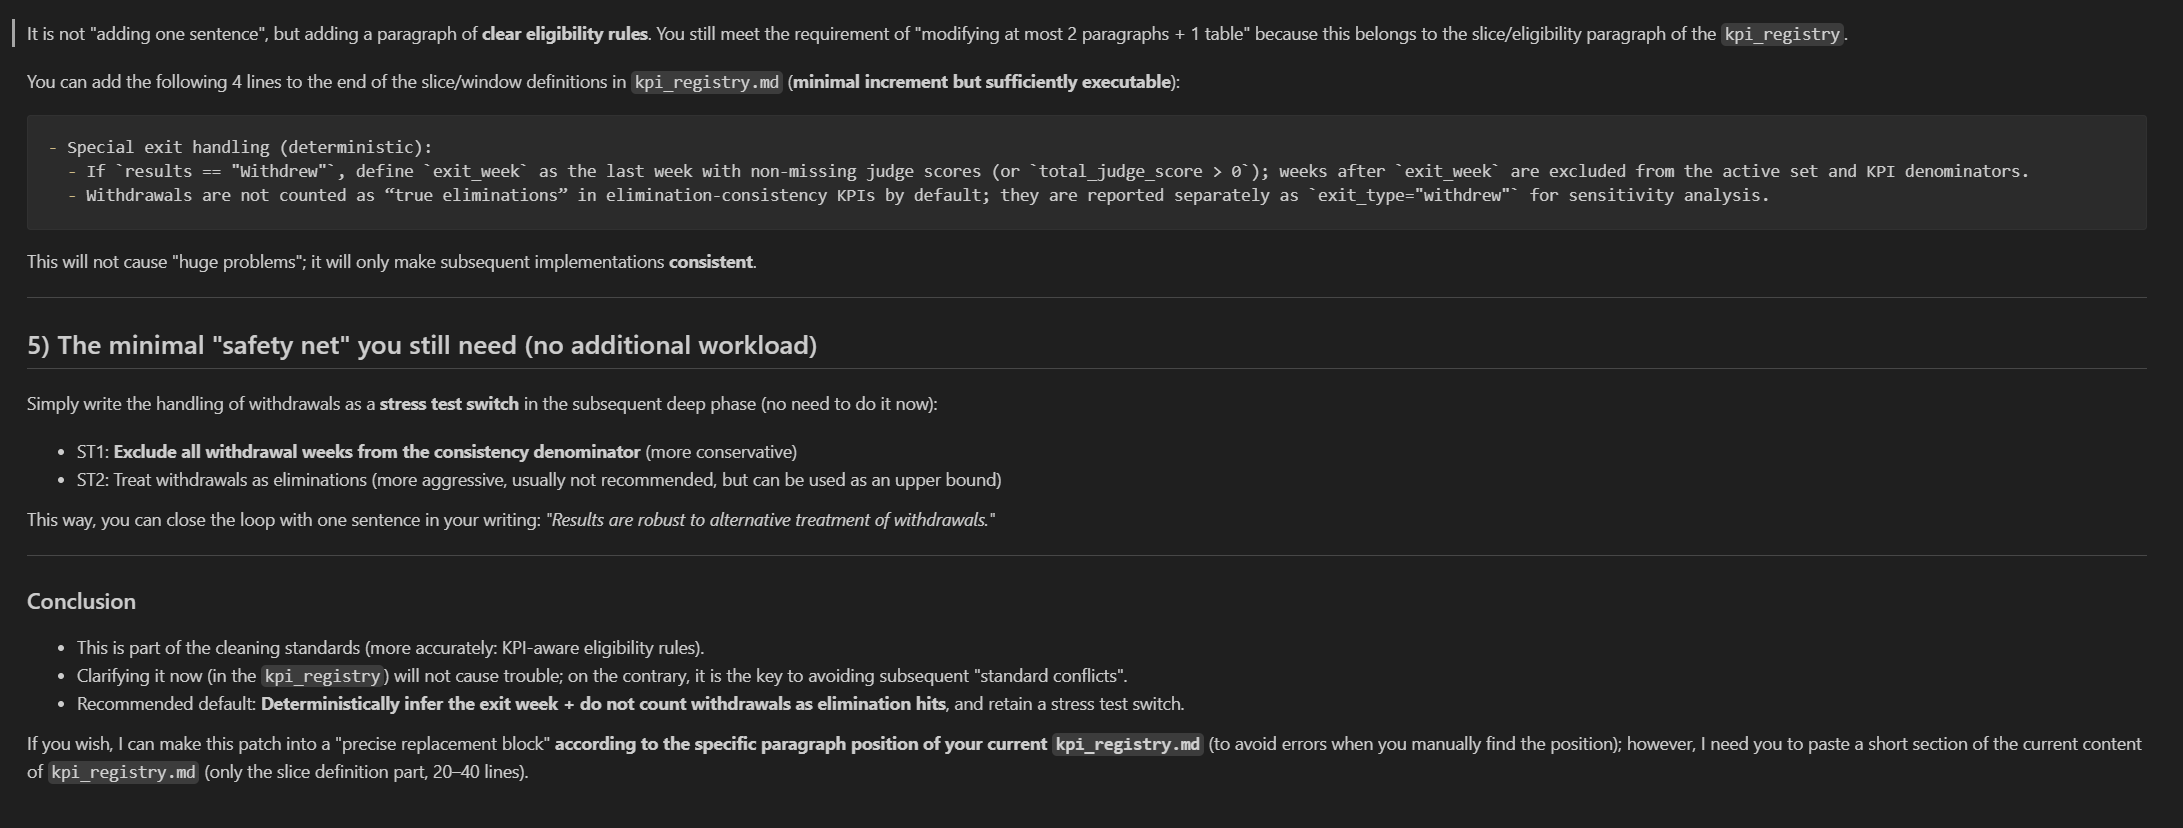
\includegraphics[width=0.9\linewidth]{report_on_use_of_ai/pho/82.png}
  \caption{ChatGPT Query 8 Output Screenshot}
  \label{fig:chatgpt_query_8_output2}
\end{figure}


\textbf{\href{https://github.com/charles65536/model2026-2/blob/main/report_on_use_of_ai/chatgpt_9_input_and_output.md}{ChatGPT Query 9:}}\\
\\
\textbf{Input:}
\begin{figure}[H]
  \centering
  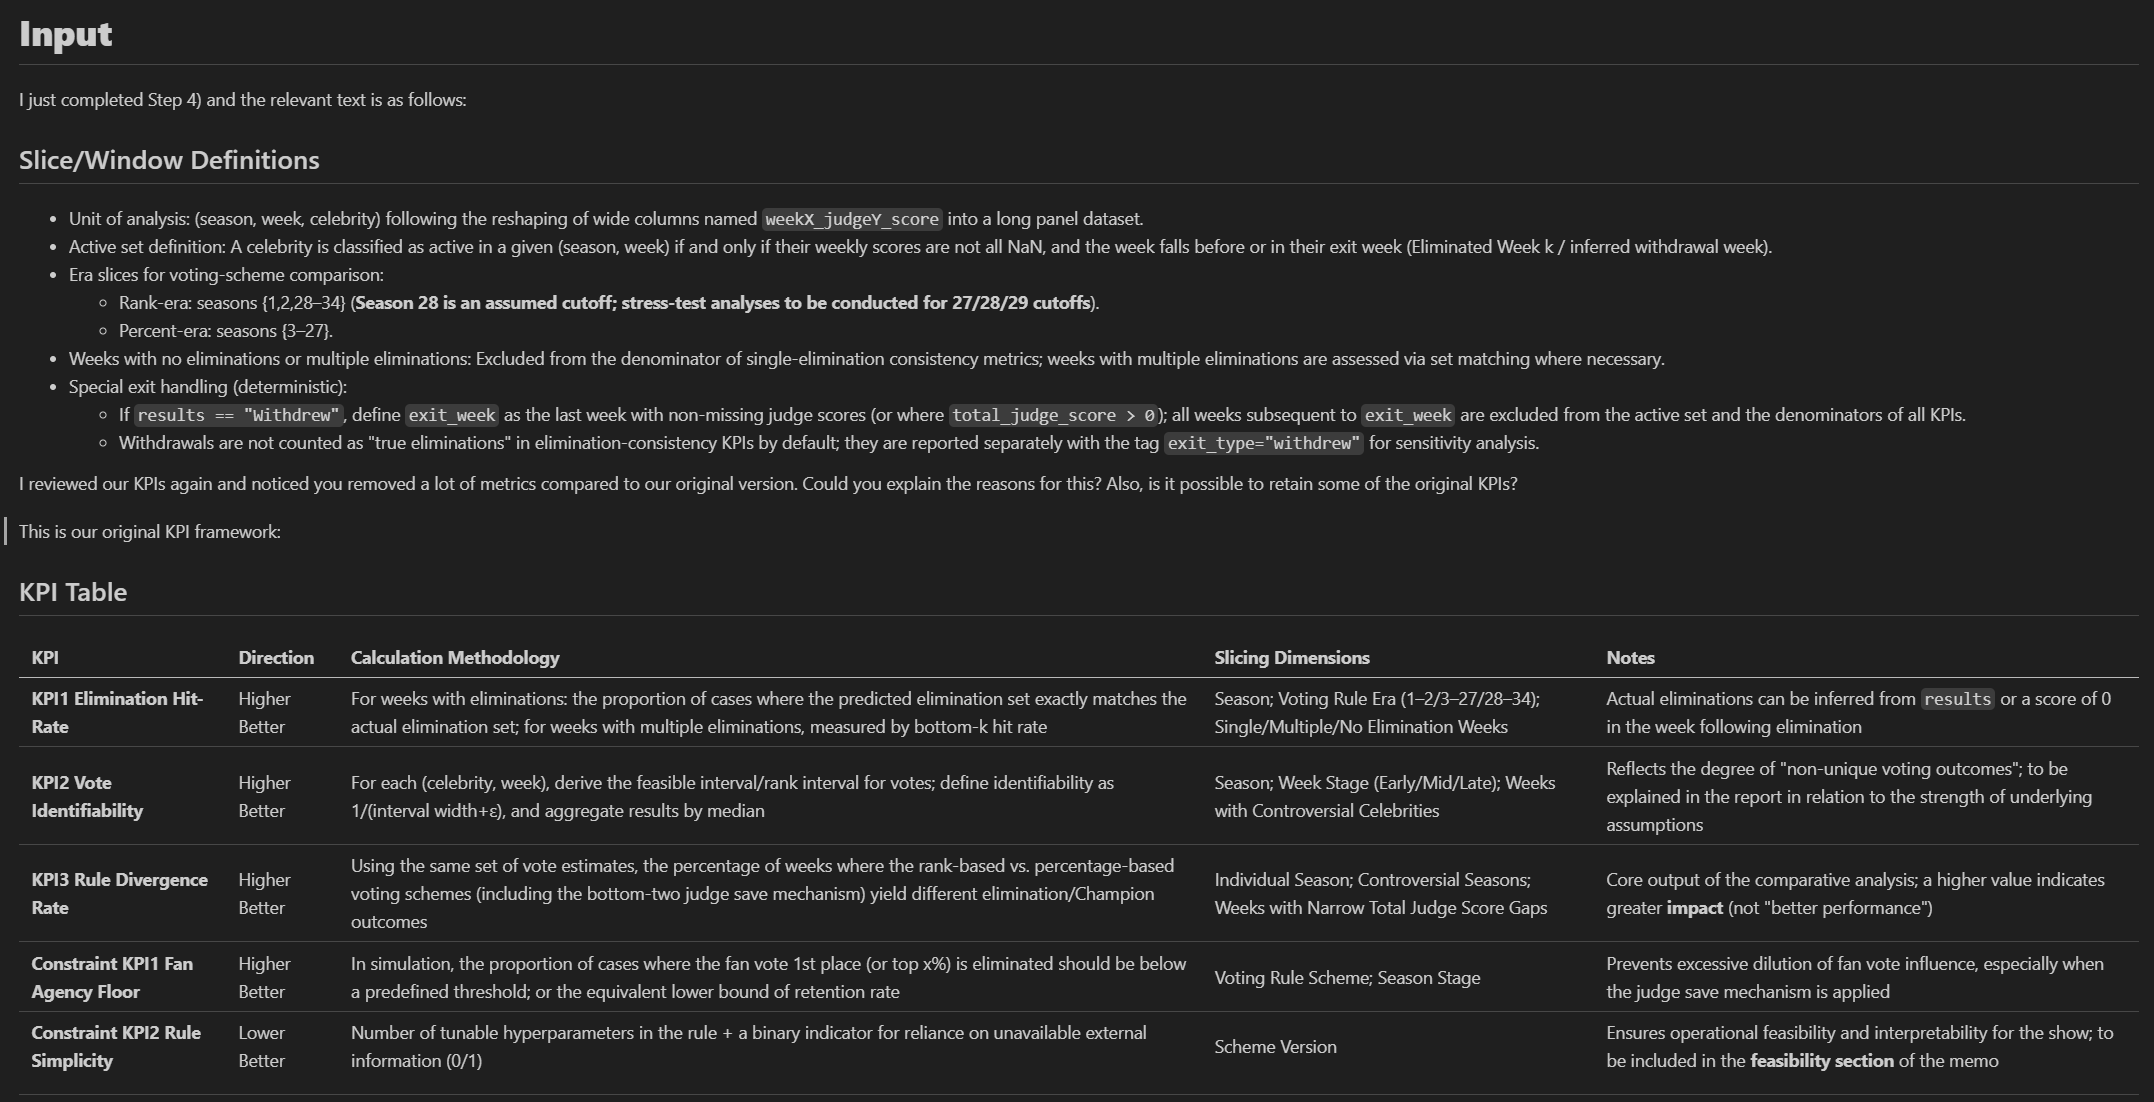
\includegraphics[width=0.9\linewidth]{report_on_use_of_ai/pho/91.png}
  \caption{ChatGPT Query 9 Input Screenshot}
  \label{fig:chatgpt_query_9_input}
\end{figure}

\textbf{Output:}
\begin{figure}[H]
  \centering
  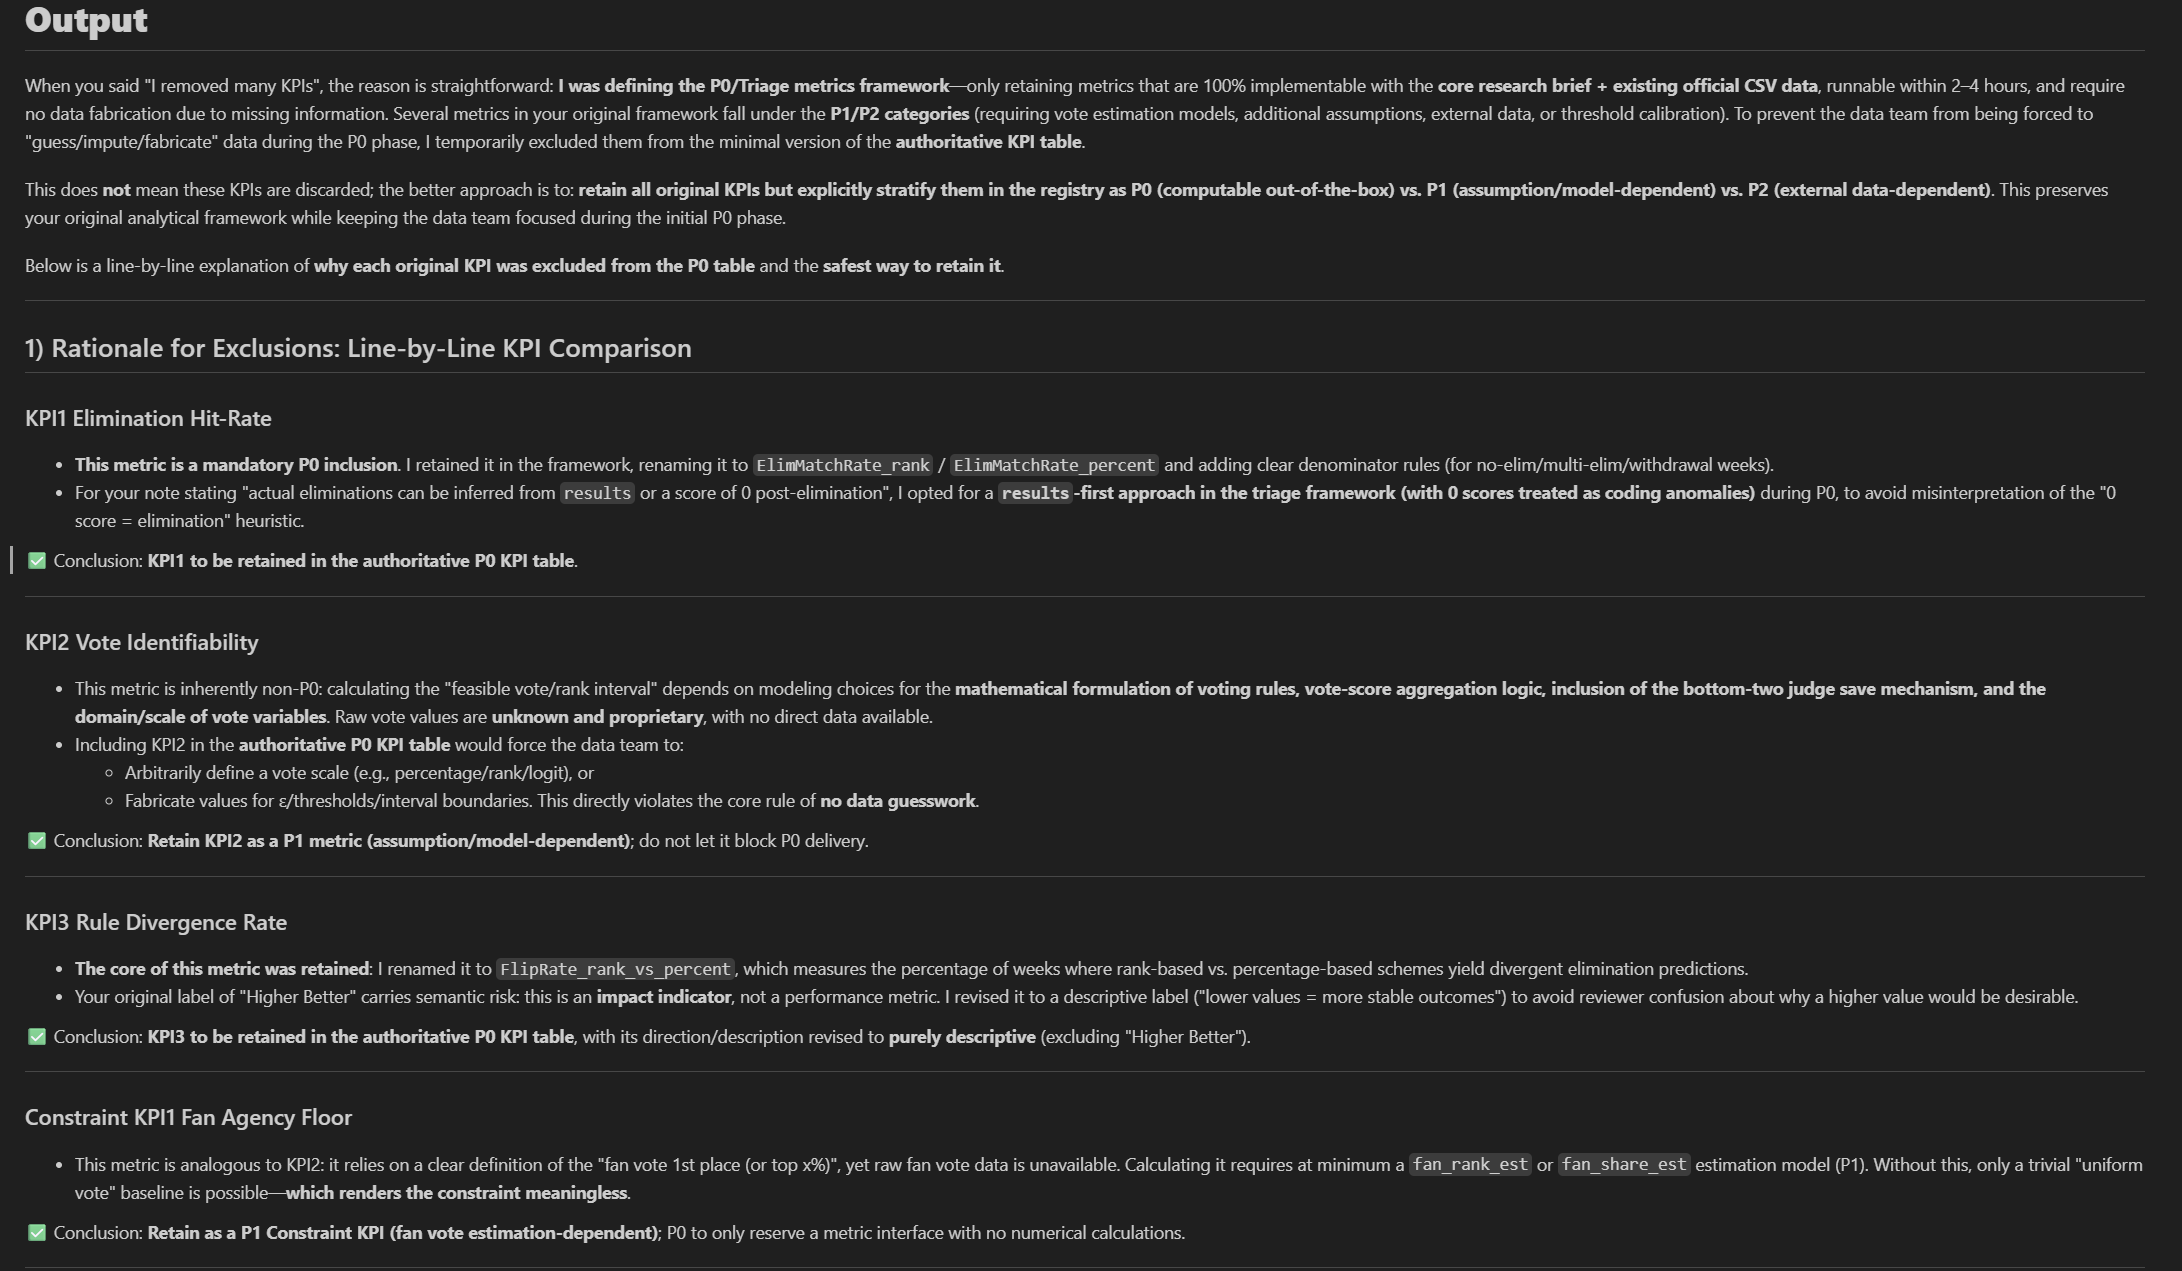
\includegraphics[width=0.9\linewidth]{report_on_use_of_ai/pho/92.png}
  \caption{ChatGPT Query 9 Output Screenshot}
  \label{fig:chatgpt_query_9_output}
\end{figure}
\begin{figure}[H]
  \centering
  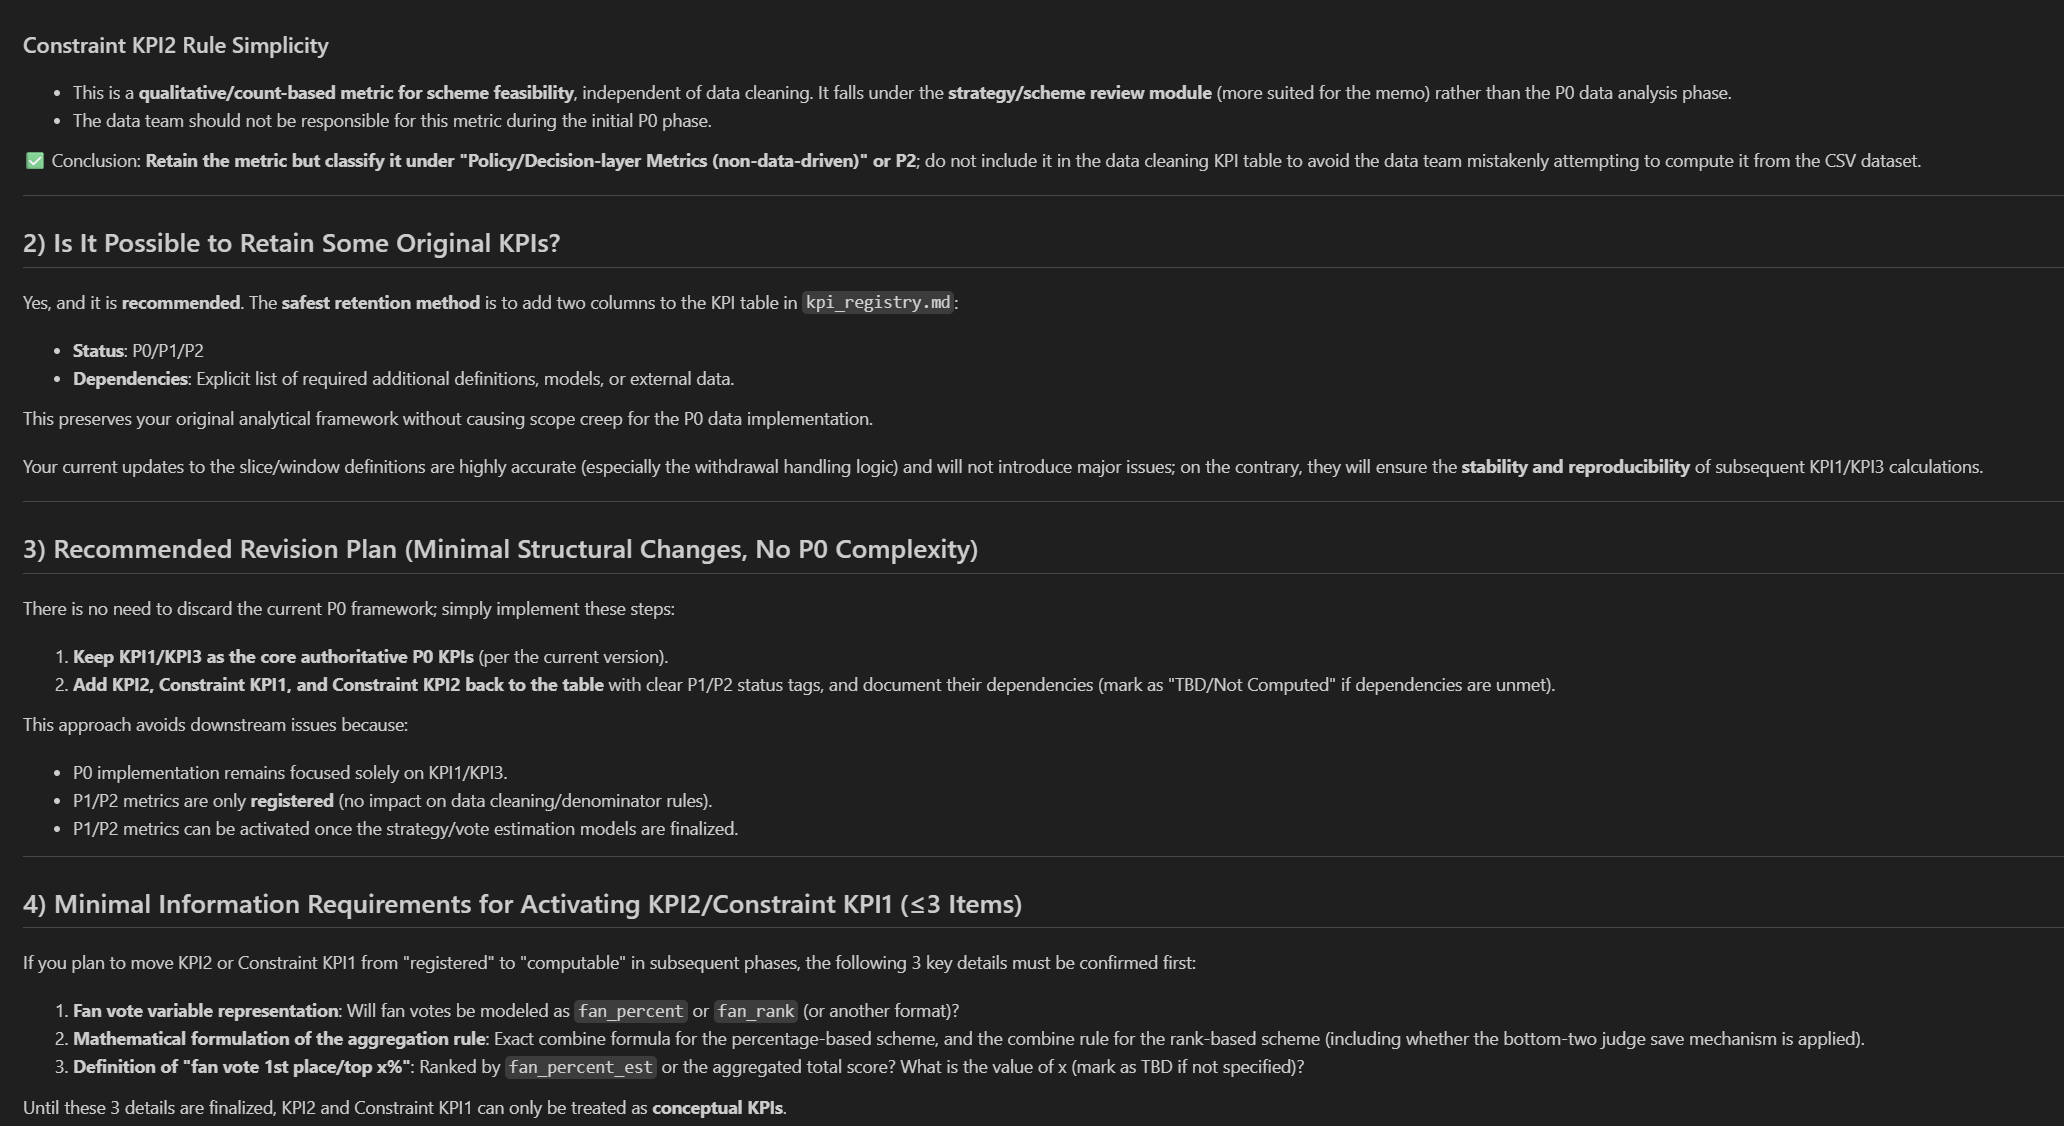
\includegraphics[width=0.9\linewidth]{report_on_use_of_ai/pho/93.png}
  \caption{ChatGPT Query 9 Output Screenshot}
  \label{fig:chatgpt_query_9_output2}
\end{figure}


\textbf{\href{https://github.com/charles65536/model2026-2/blob/main/report_on_use_of_ai/chatgpt_10_input_and_output.md}{ChatGPT Query 10:}}\\
\textbf{Input:}

\begin{figure}[H]
  \centering
  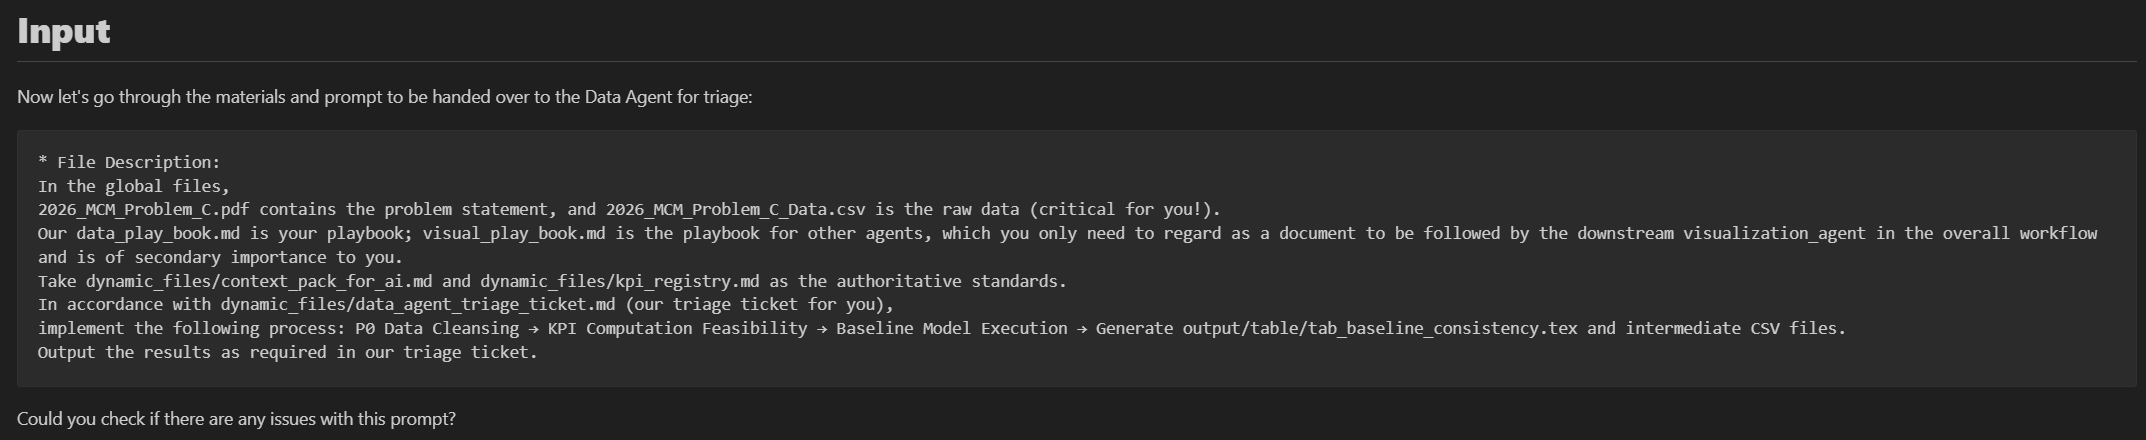
\includegraphics[width=0.9\linewidth]{report_on_use_of_ai/pho/101.png}
  \caption{ChatGPT Query 10 Input Screenshot}
  \label{fig:chatgpt_query_10_input}
\end{figure}

\textbf{Output:}
\begin{figure}[H]
  \centering
  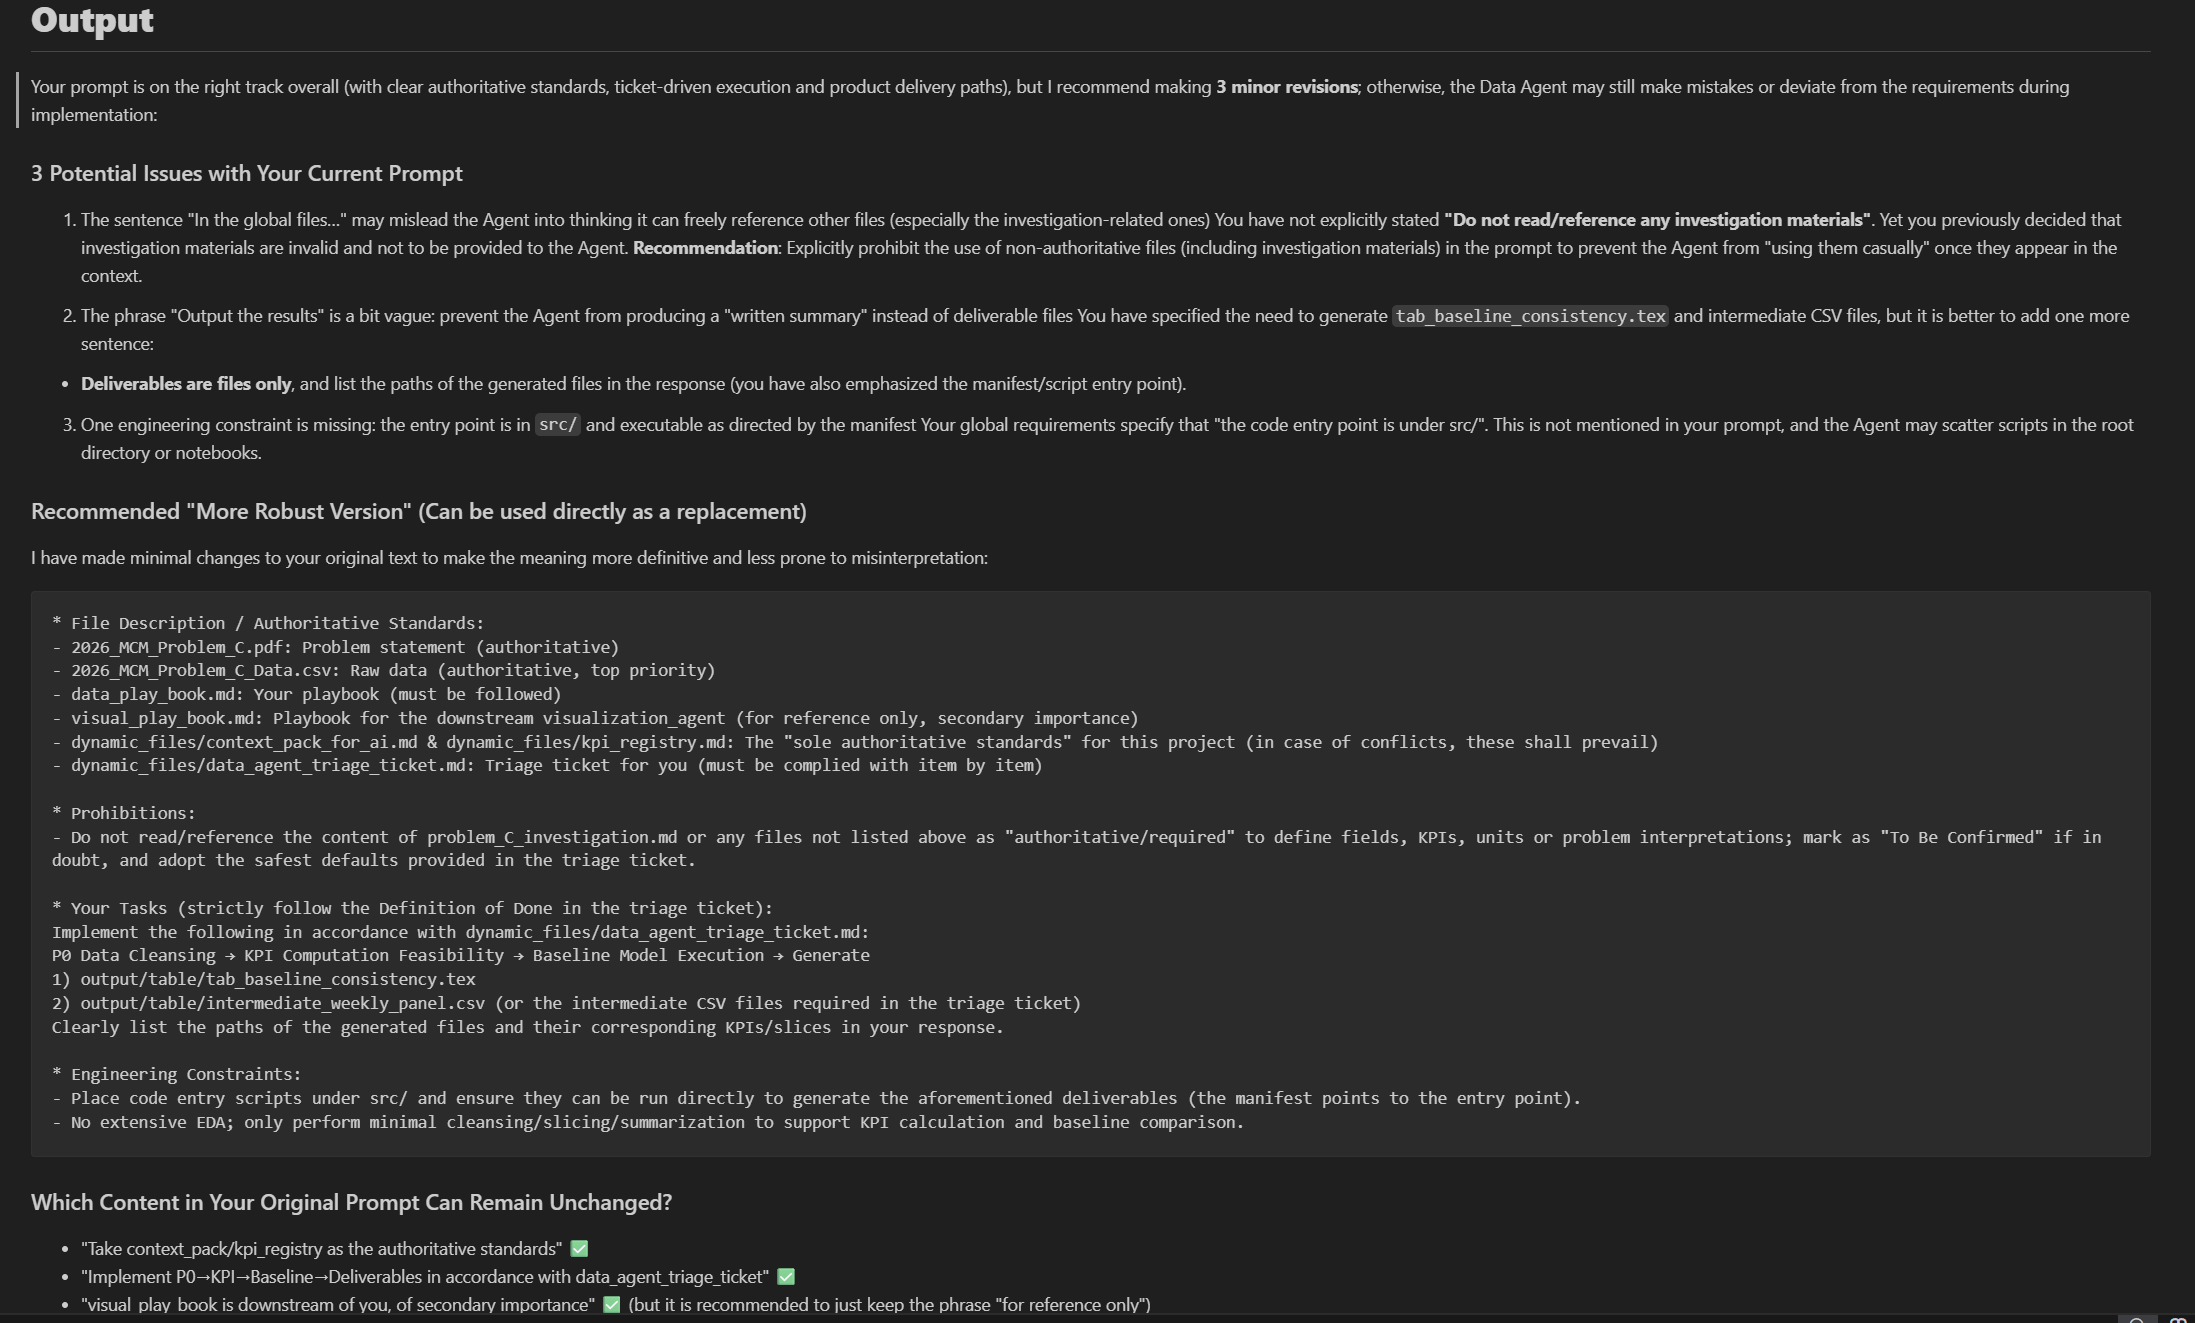
\includegraphics[width=0.9\linewidth]{report_on_use_of_ai/pho/102.png}
  \caption{ChatGPT Query 10 Output Screenshot}
  \label{fig:chatgpt_query_10_output}
\end{figure}

\begin{figure}[H]
  \centering
  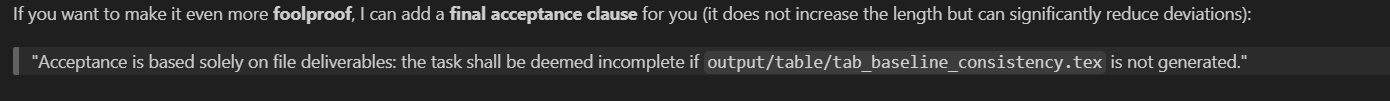
\includegraphics[width=0.9\linewidth]{report_on_use_of_ai/pho/103.png}
  \caption{ChatGPT Query 10 Output Screenshot}
  \label{fig:chatgpt_query_10_output2}
\end{figure}


\textbf{\href{https://github.com/charles65536/model2026-2/blob/main/report_on_use_of_ai/chatgpt_11_input_and_output.md}{ChatGPT Query 11:}}\\
\textbf{Input:}

\begin{figure}[H]
  \centering
  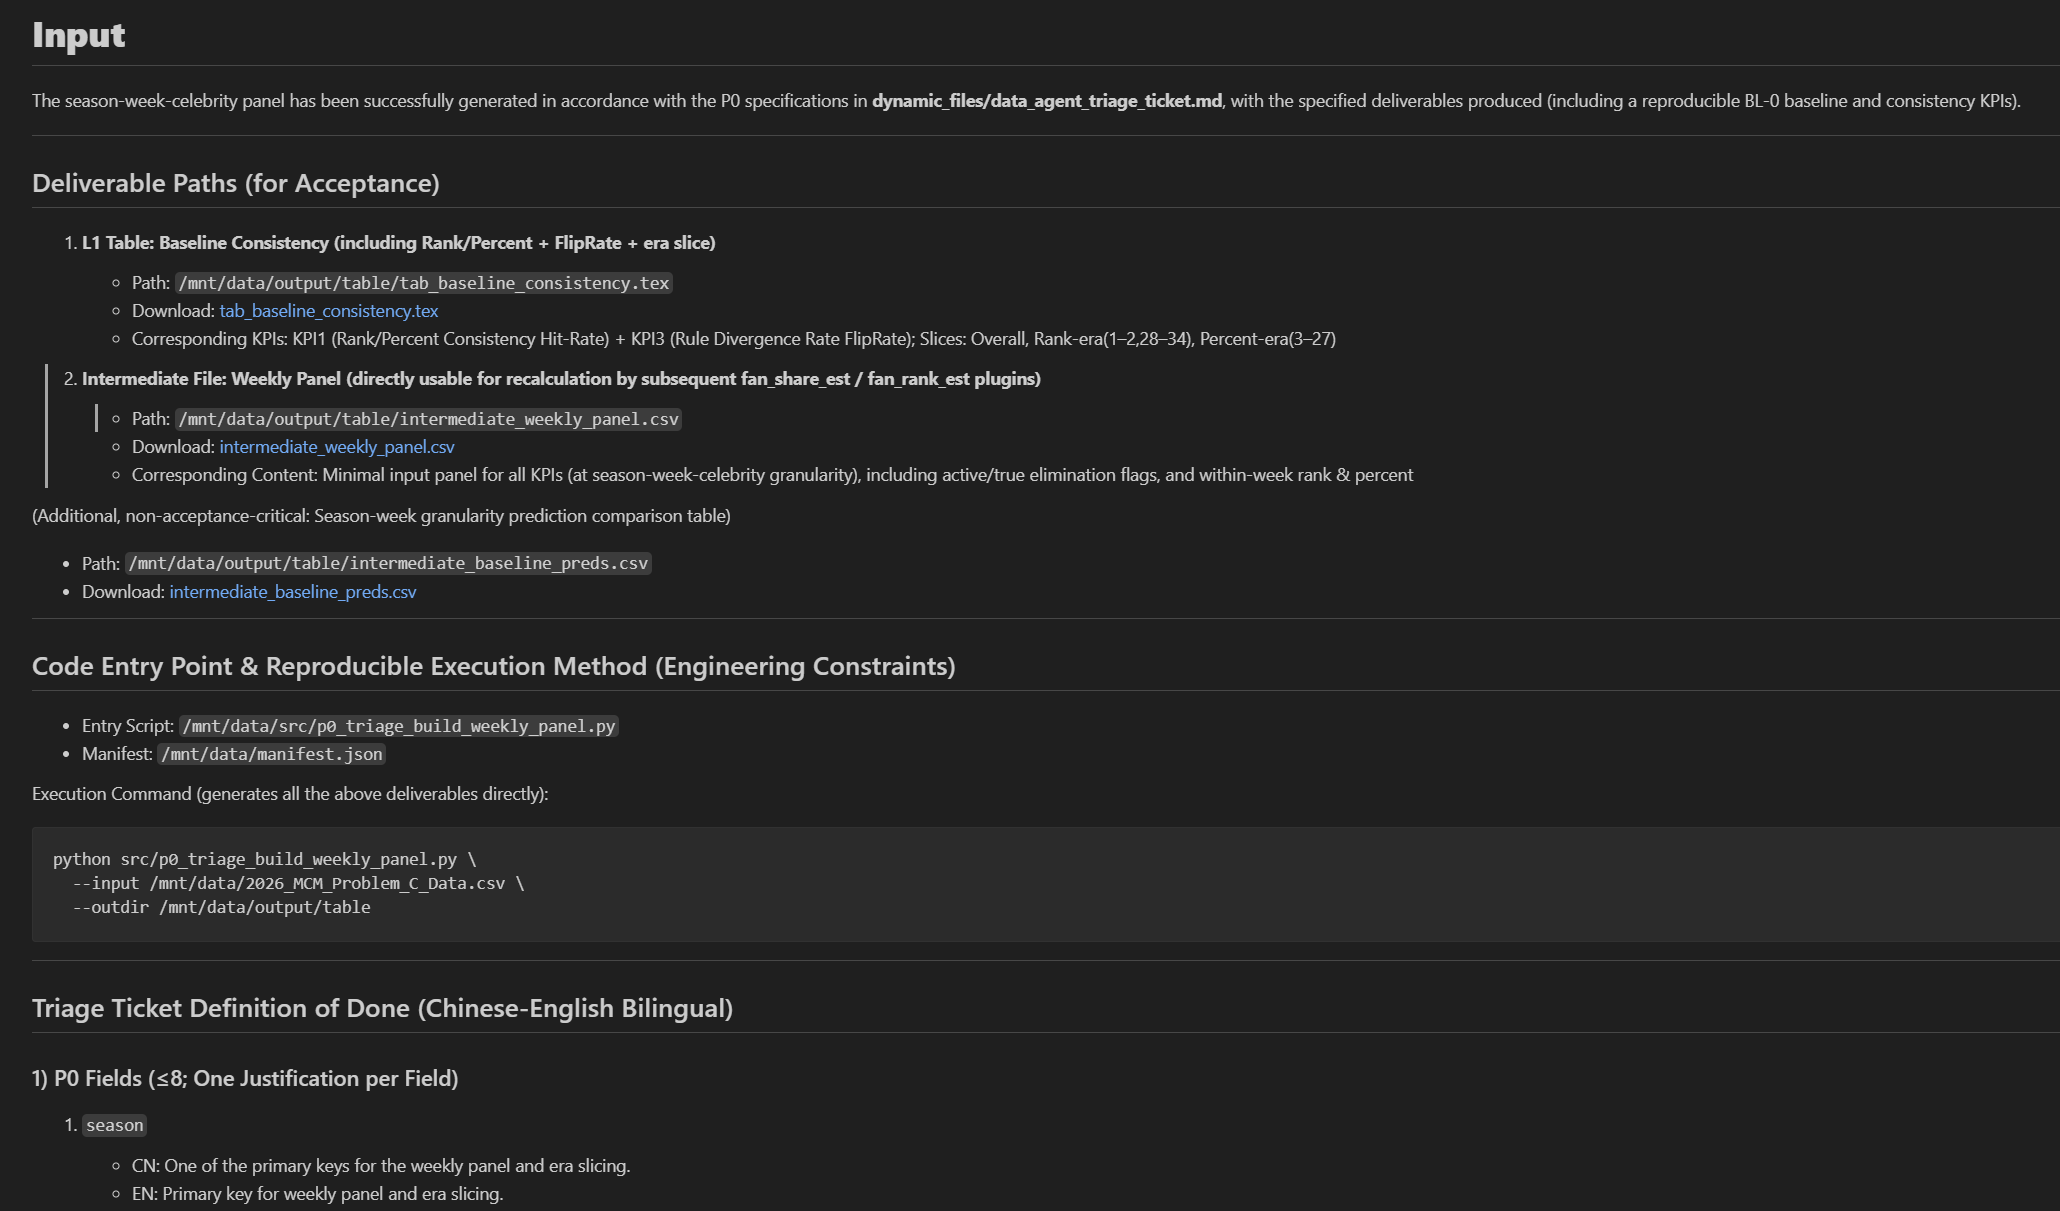
\includegraphics[width=0.9\linewidth]{report_on_use_of_ai/pho/111.png}
  \caption{ChatGPT Query 11 Input Screenshot}
  \label{fig:chatgpt_query_11_input}
\end{figure}

\textbf{Output:}
\begin{figure}[H]
  \centering
  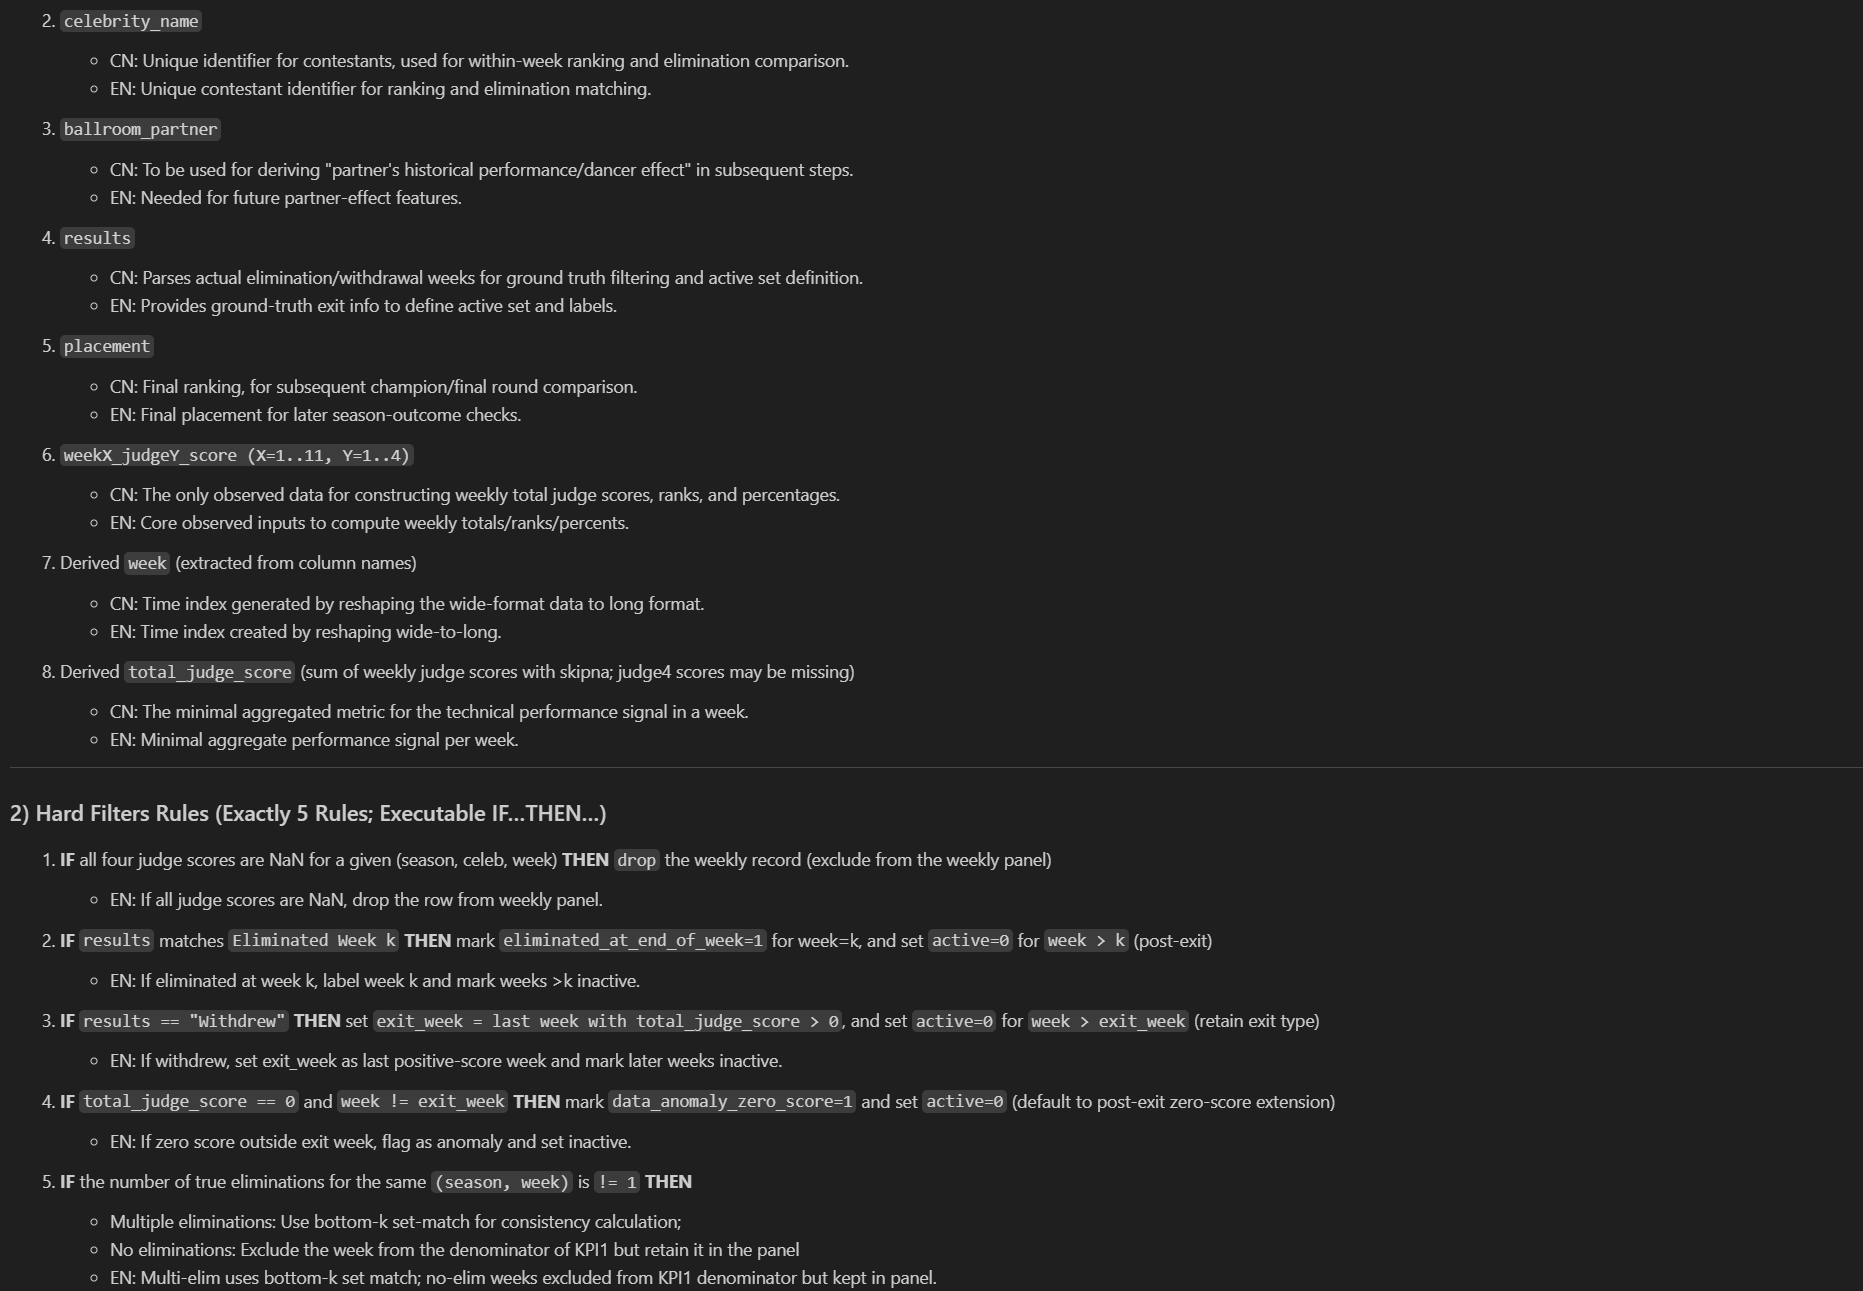
\includegraphics[width=0.9\linewidth]{report_on_use_of_ai/pho/112.png}
  \caption{ChatGPT Query 11 Output Screenshot}
  \label{fig:chatgpt_query_11_output}
\end{figure}
\begin{figure}[H]
  \centering
  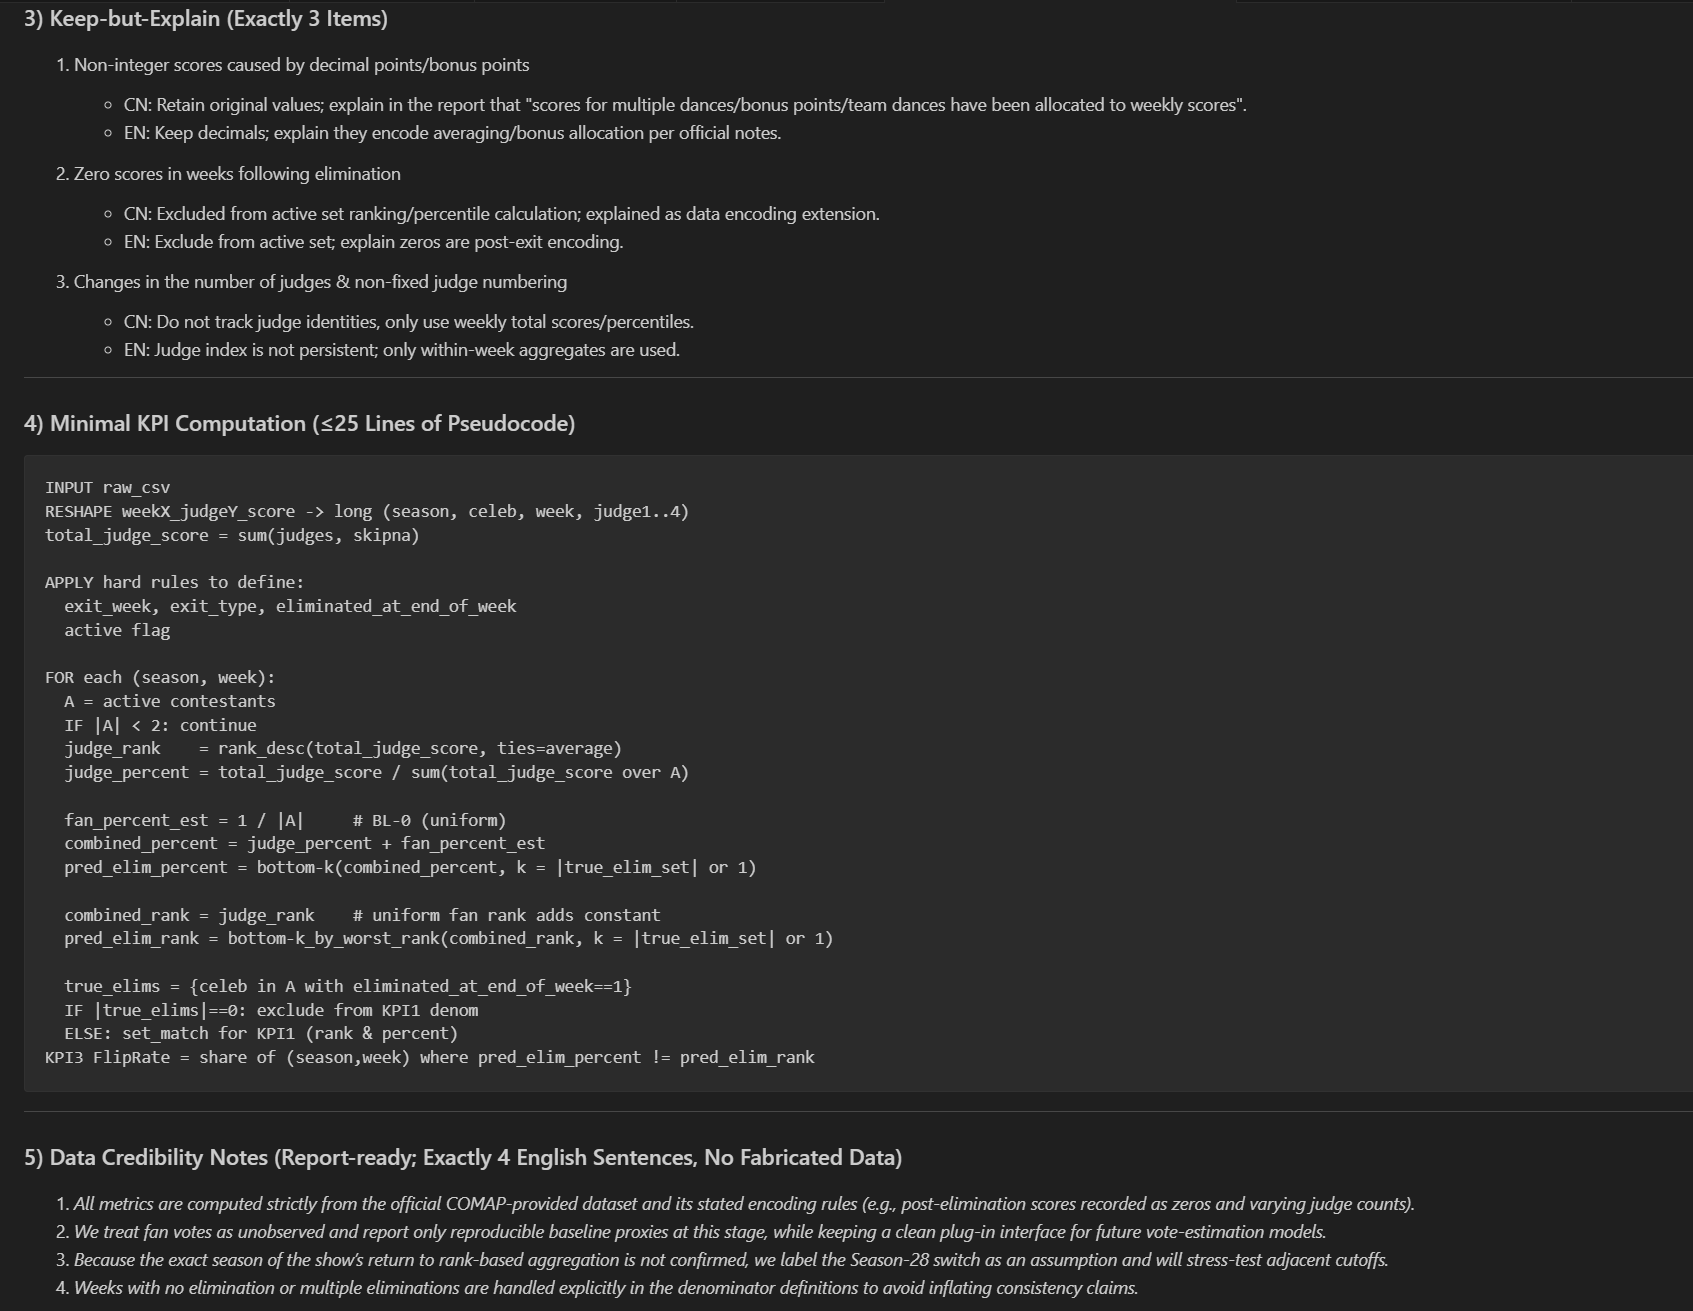
\includegraphics[width=0.9\linewidth]{report_on_use_of_ai/pho/113.png}
  \caption{ChatGPT Query 11 Output Screenshot}
  \label{fig:chatgpt_query_11_output2}
\end{figure}




\textbf{\href{https://github.com/charles65536/model2026-2/blob/main/report_on_use_of_ai/chatgpt_12_input_and_output.md}{ChatGPT Query 12:}}\\
\textbf{Input:}
\begin{figure}[H]
  \centering
  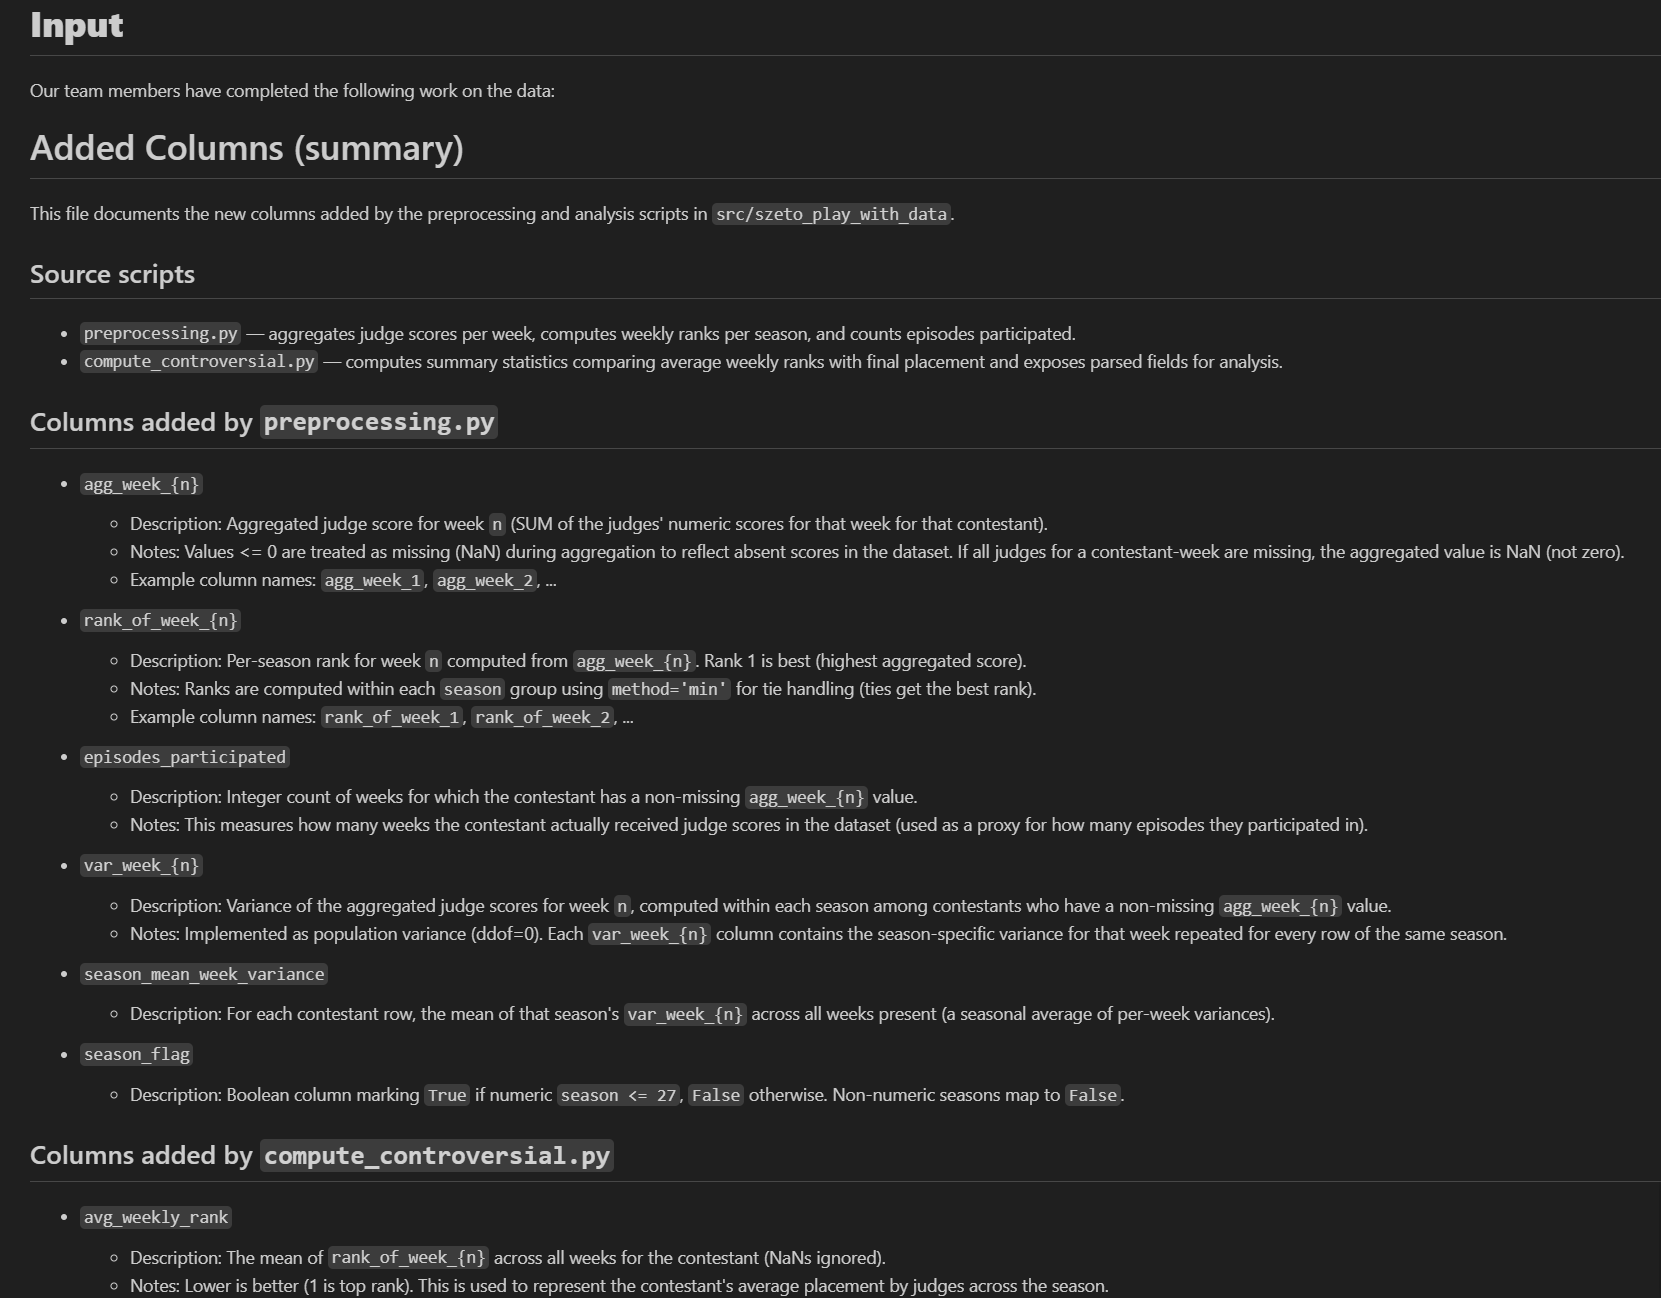
\includegraphics[width=0.9\linewidth]{report_on_use_of_ai/pho/121.png}
  \caption{ChatGPT Query 12 Input Screenshot}
  \label{fig:chatgpt_query_12_input}
\end{figure}

\textbf{Output:}
\begin{figure}[H]
  \centering
  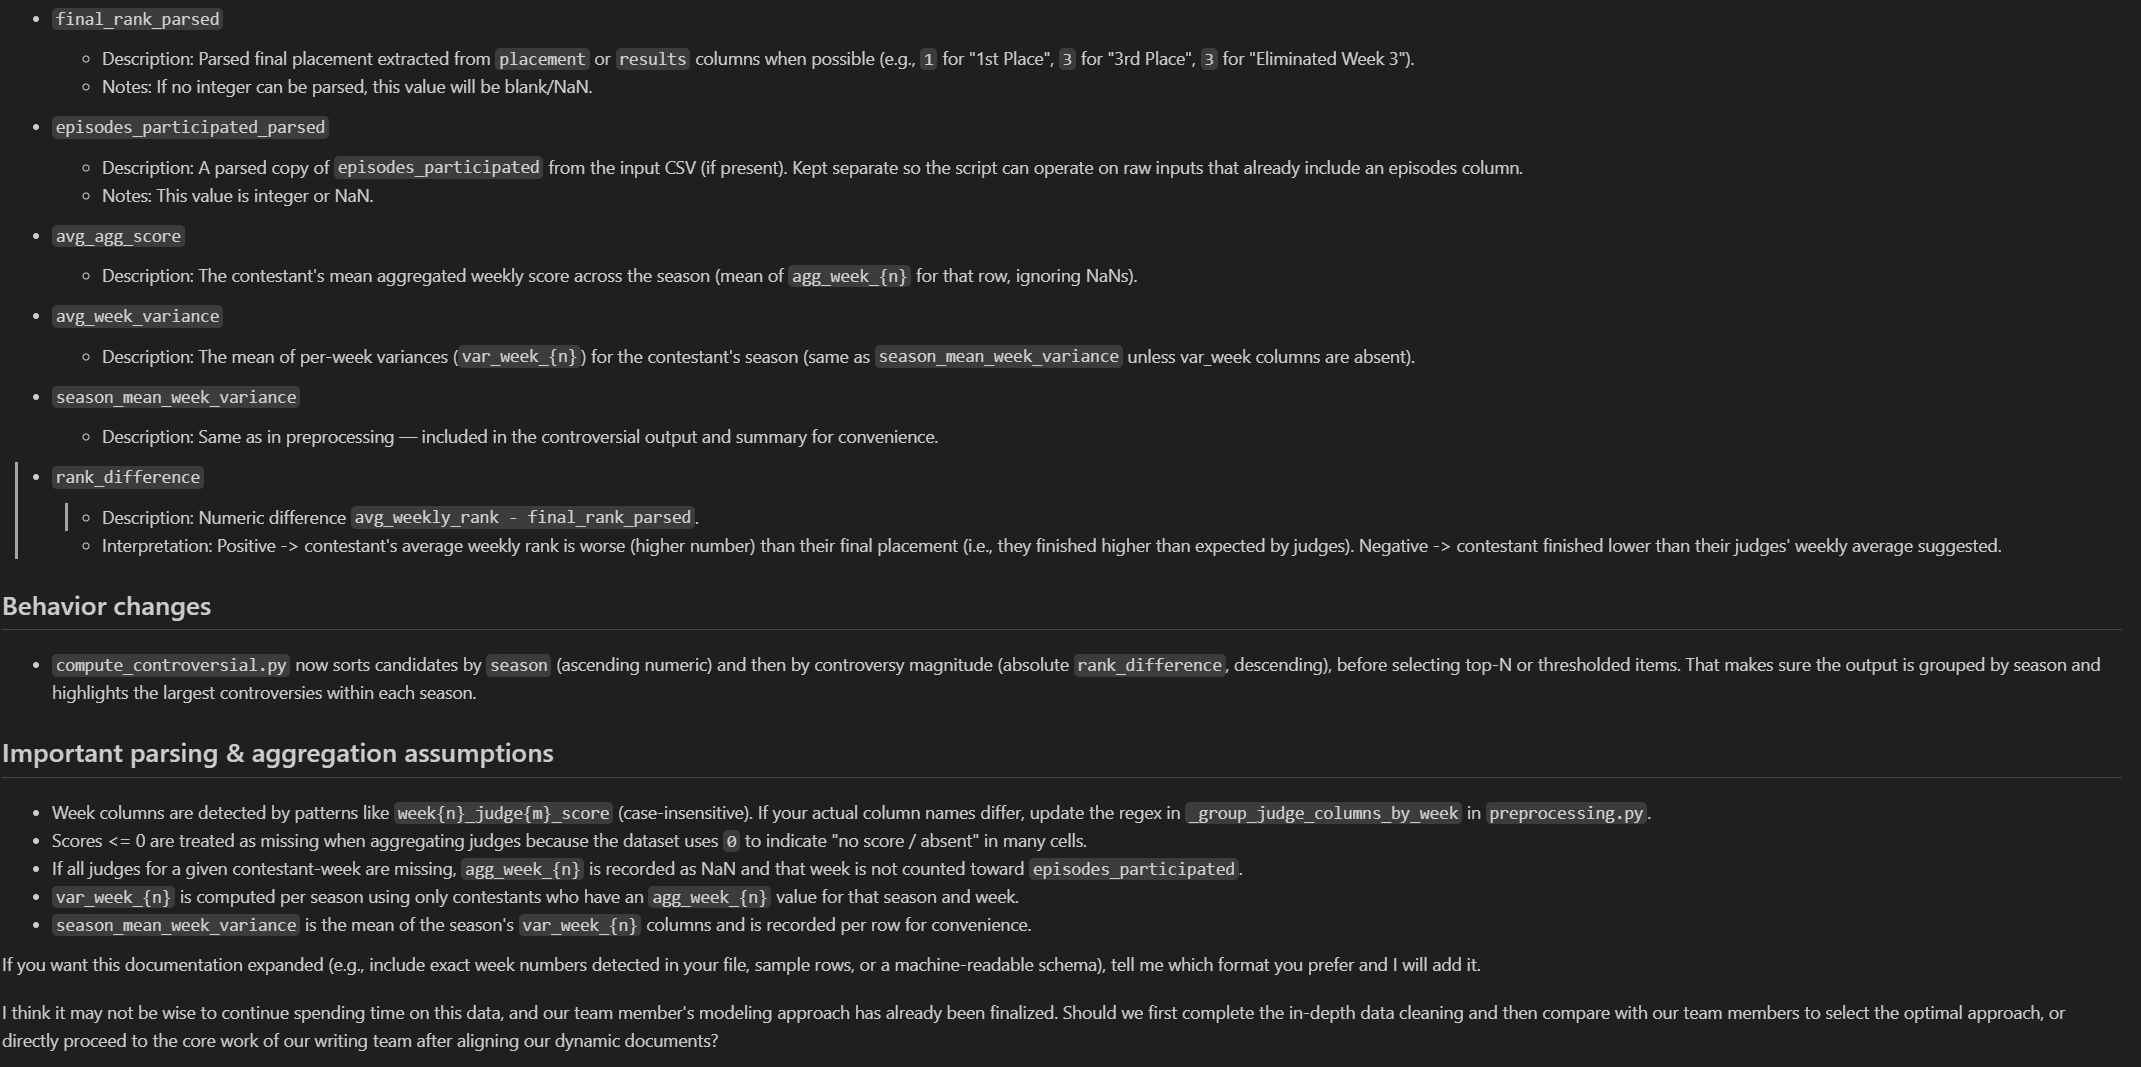
\includegraphics[width=0.9\linewidth]{report_on_use_of_ai/pho/122.png}
  \caption{ChatGPT Query 12 Output Screenshot}
  \label{fig:chatgpt_query_12_output}
\end{figure}
\begin{figure}[H]
  \centering
  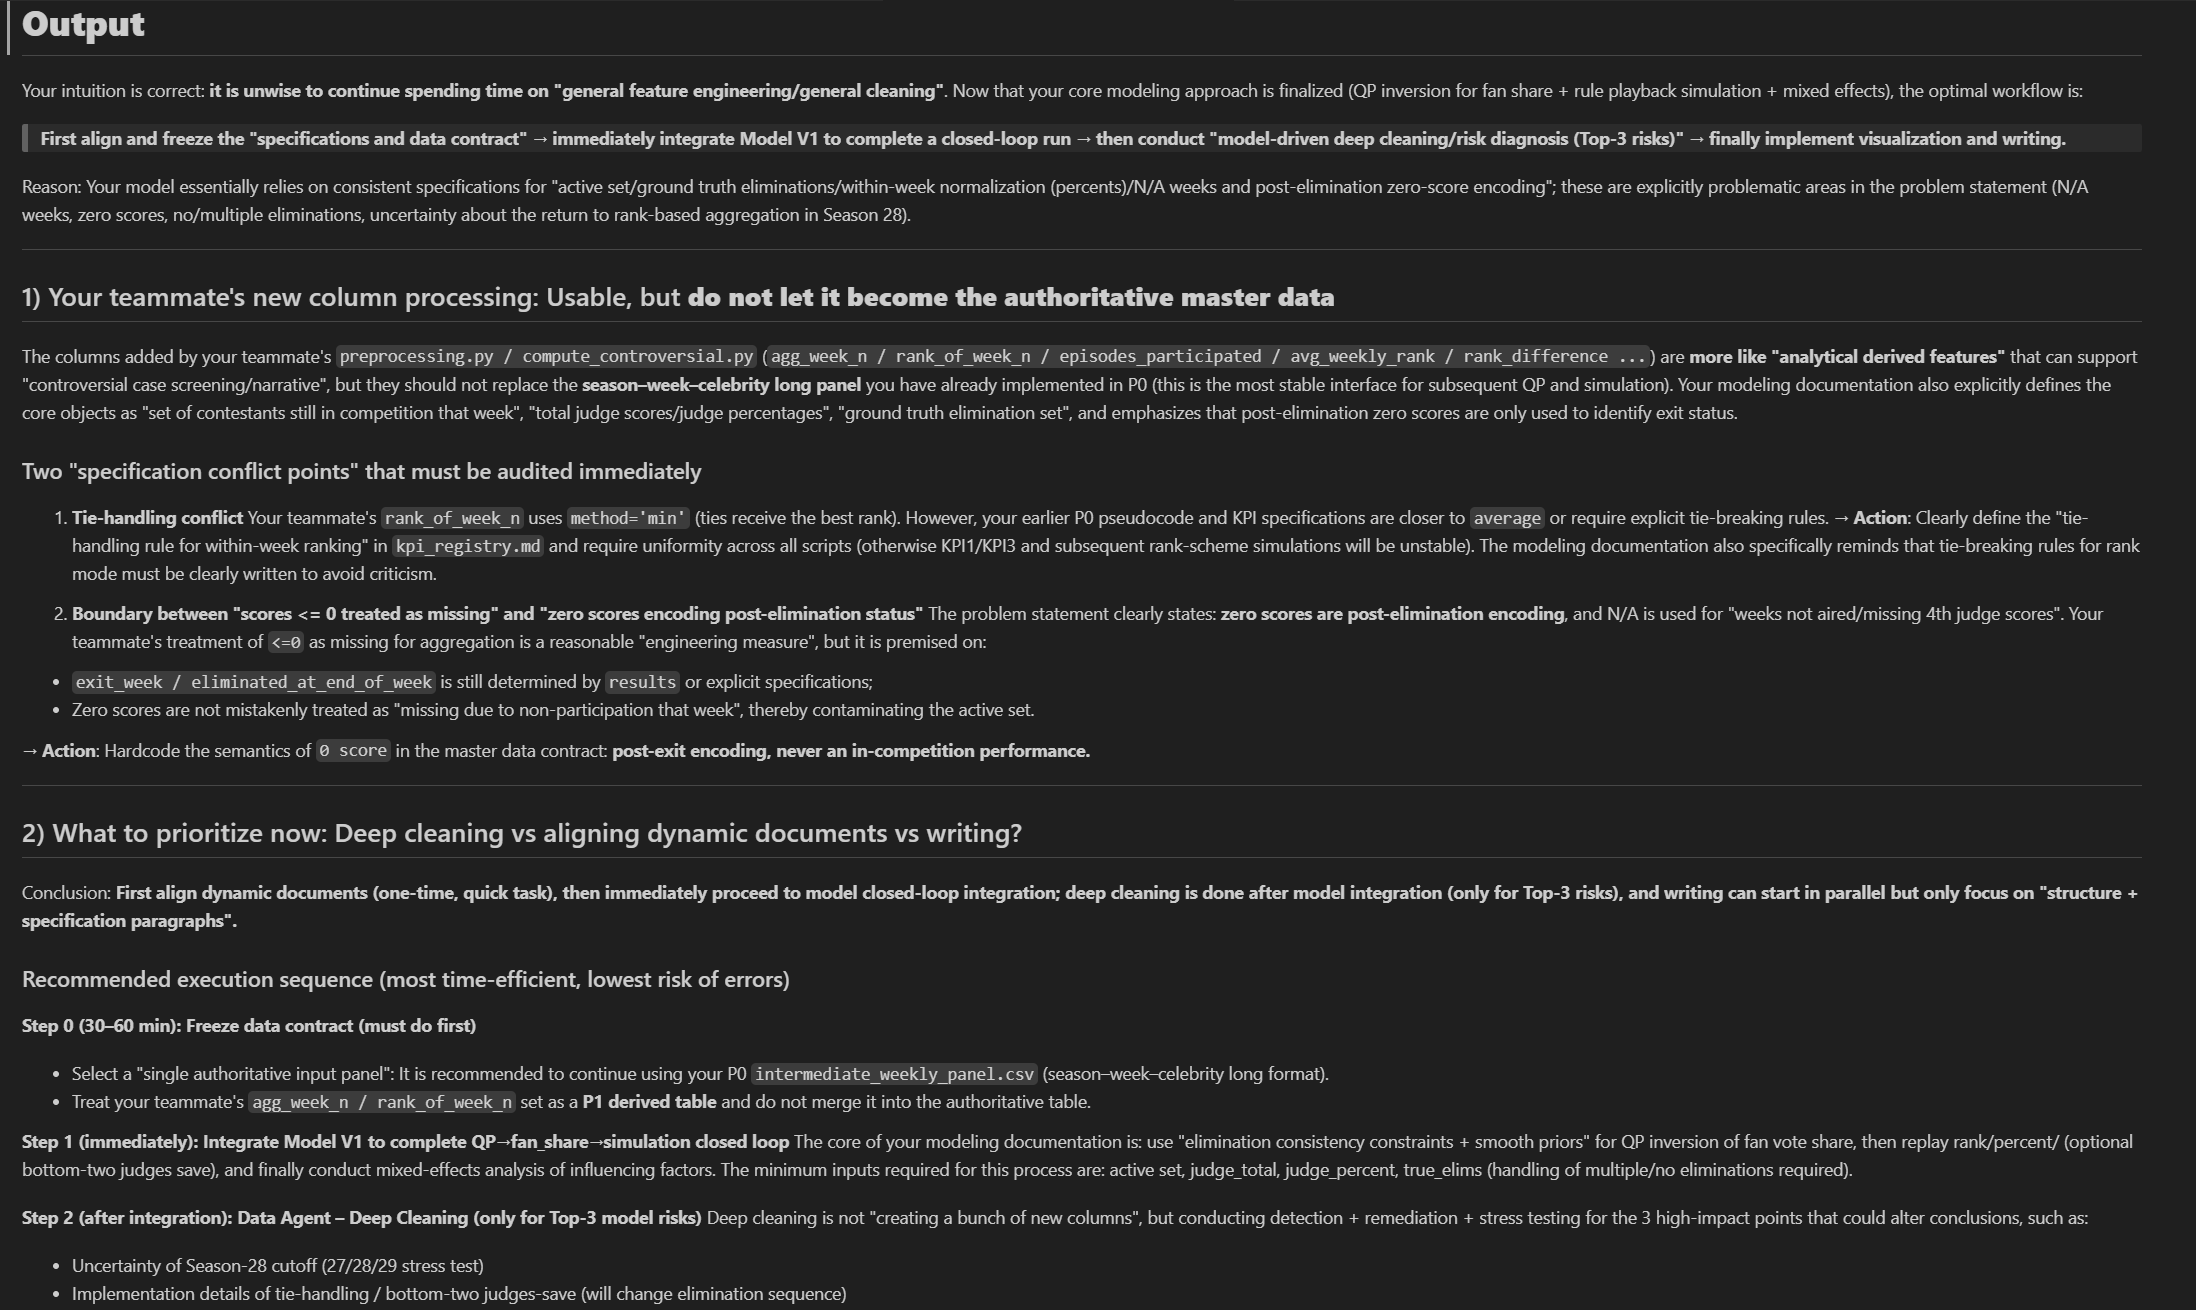
\includegraphics[width=0.9\linewidth]{report_on_use_of_ai/pho/123.png}
  \caption{ChatGPT Query 12 Output Screenshot}
  \label{fig:chatgpt_query_12_output_2}
\end{figure}
\begin{figure}[H]
  \centering
  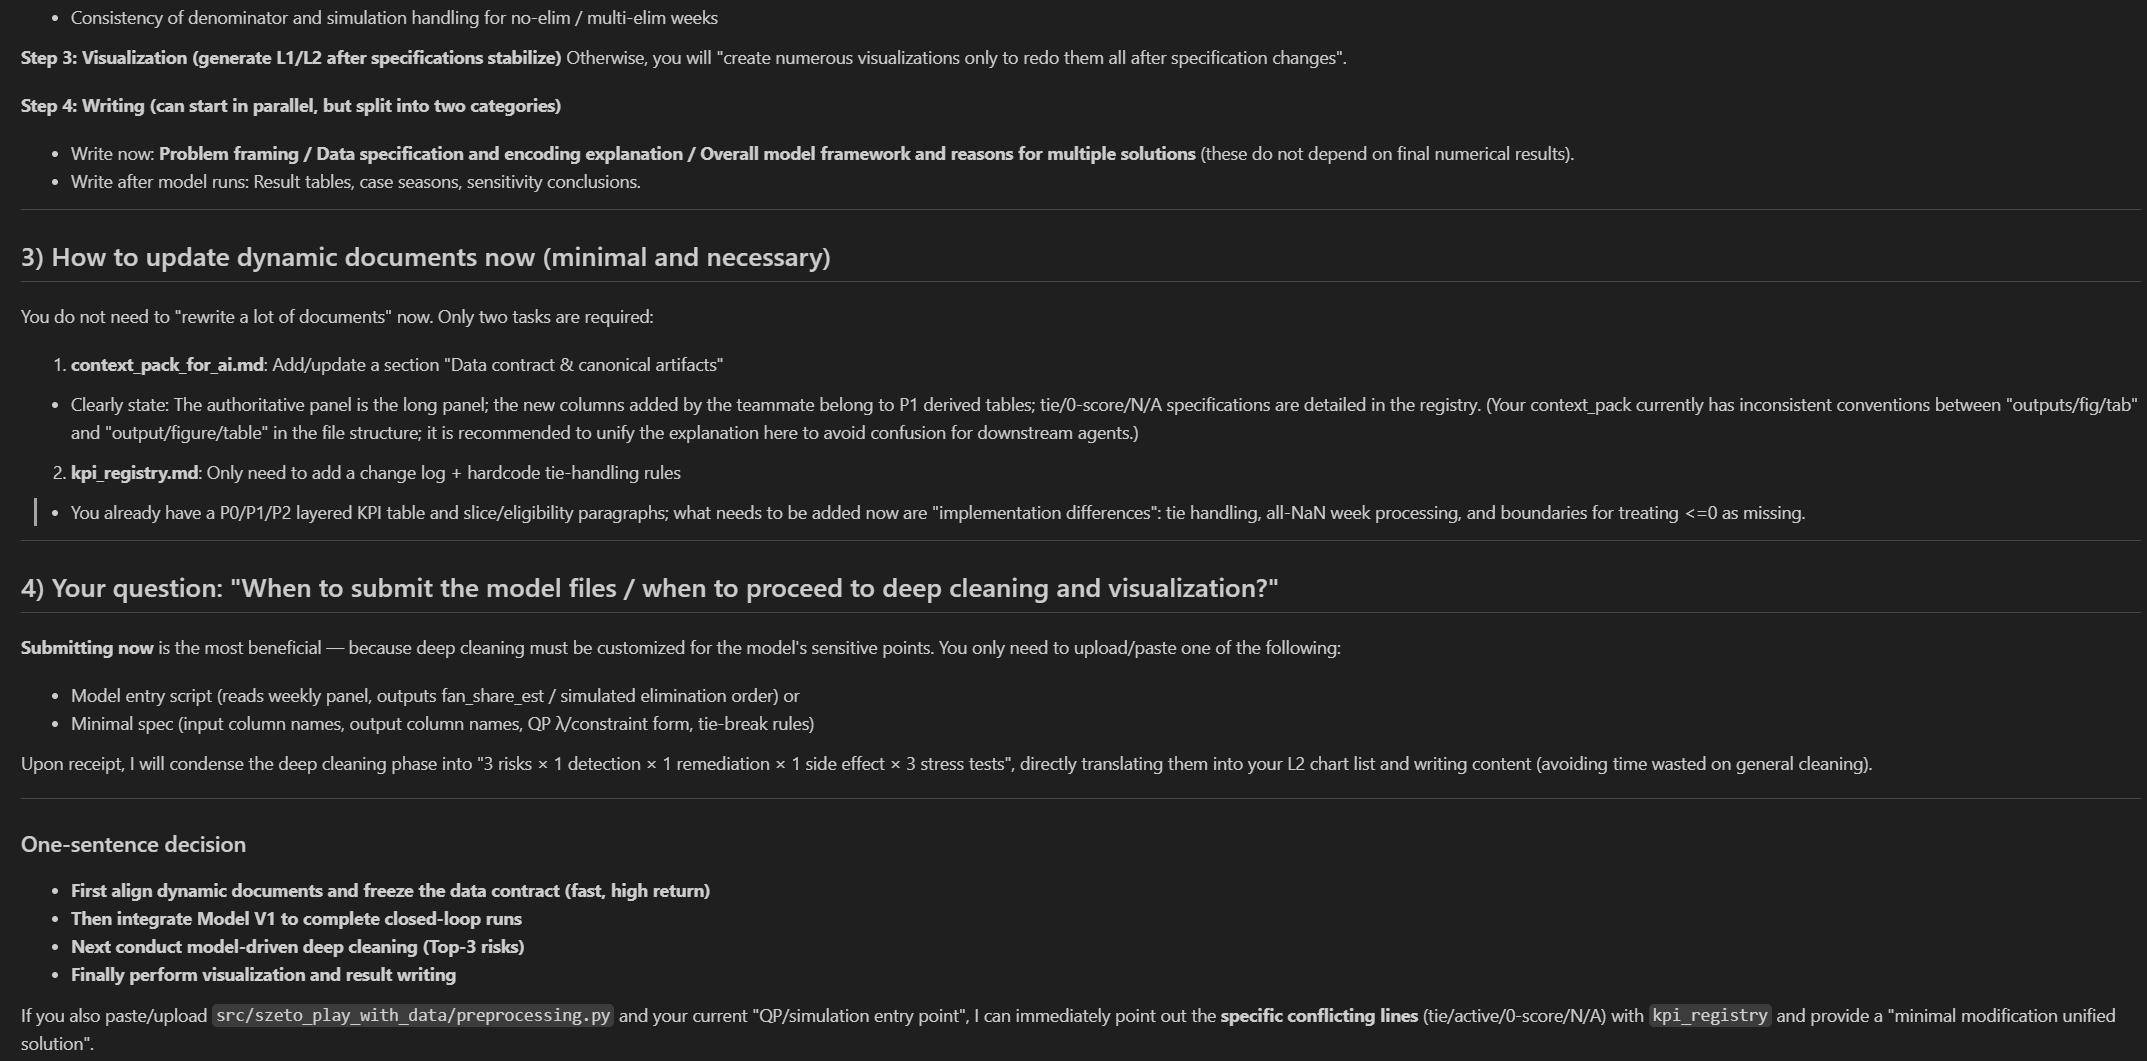
\includegraphics[width=0.9\linewidth]{report_on_use_of_ai/pho/124.png}
  \caption{ChatGPT Query 12 Output Screenshot}
  \label{fig:chatgpt_query_12_output_3}
\end{figure}




\textbf{\href{https://github.com/charles65536/model2026-2/blob/main/report_on_use_of_ai/chatgpt_13_input_and_output.md}{ChatGPT Query 13:}}\\
\textbf{Input:}
So let me sort out what we need to do now:
First step: Align our specifications. You mentioned freezing and sticking to our core data pipeline, but actually I don't think this is necessary. Because after my teammate makes modifications, they will put their work in their own folder on GitHub, and mine will go into my folder. Even though we're in the same GitHub repository, we can cross-check each other's work later---it'll be like mutual supplementation.
Second step: Integrating Model V1. I don't quite understand this part—does V1 refer to a code file (not a DOCX document) that will make the model we've designed actually run? Is that the right understanding?
Then third step: Conduct in-depth data cleaning, followed by visualization and finalizing the writing. Is this the correct workflow?
I also have another question: Earlier, we identified two risks of inconsistent specifications, right? Well, I suggest we fix these specification inconsistencies first—preferably by modifying the code. I'll send you the code, and could you guide me on exactly what needs to be changed?\\
\textbf{Output:}
\begin{figure}
  \centering
  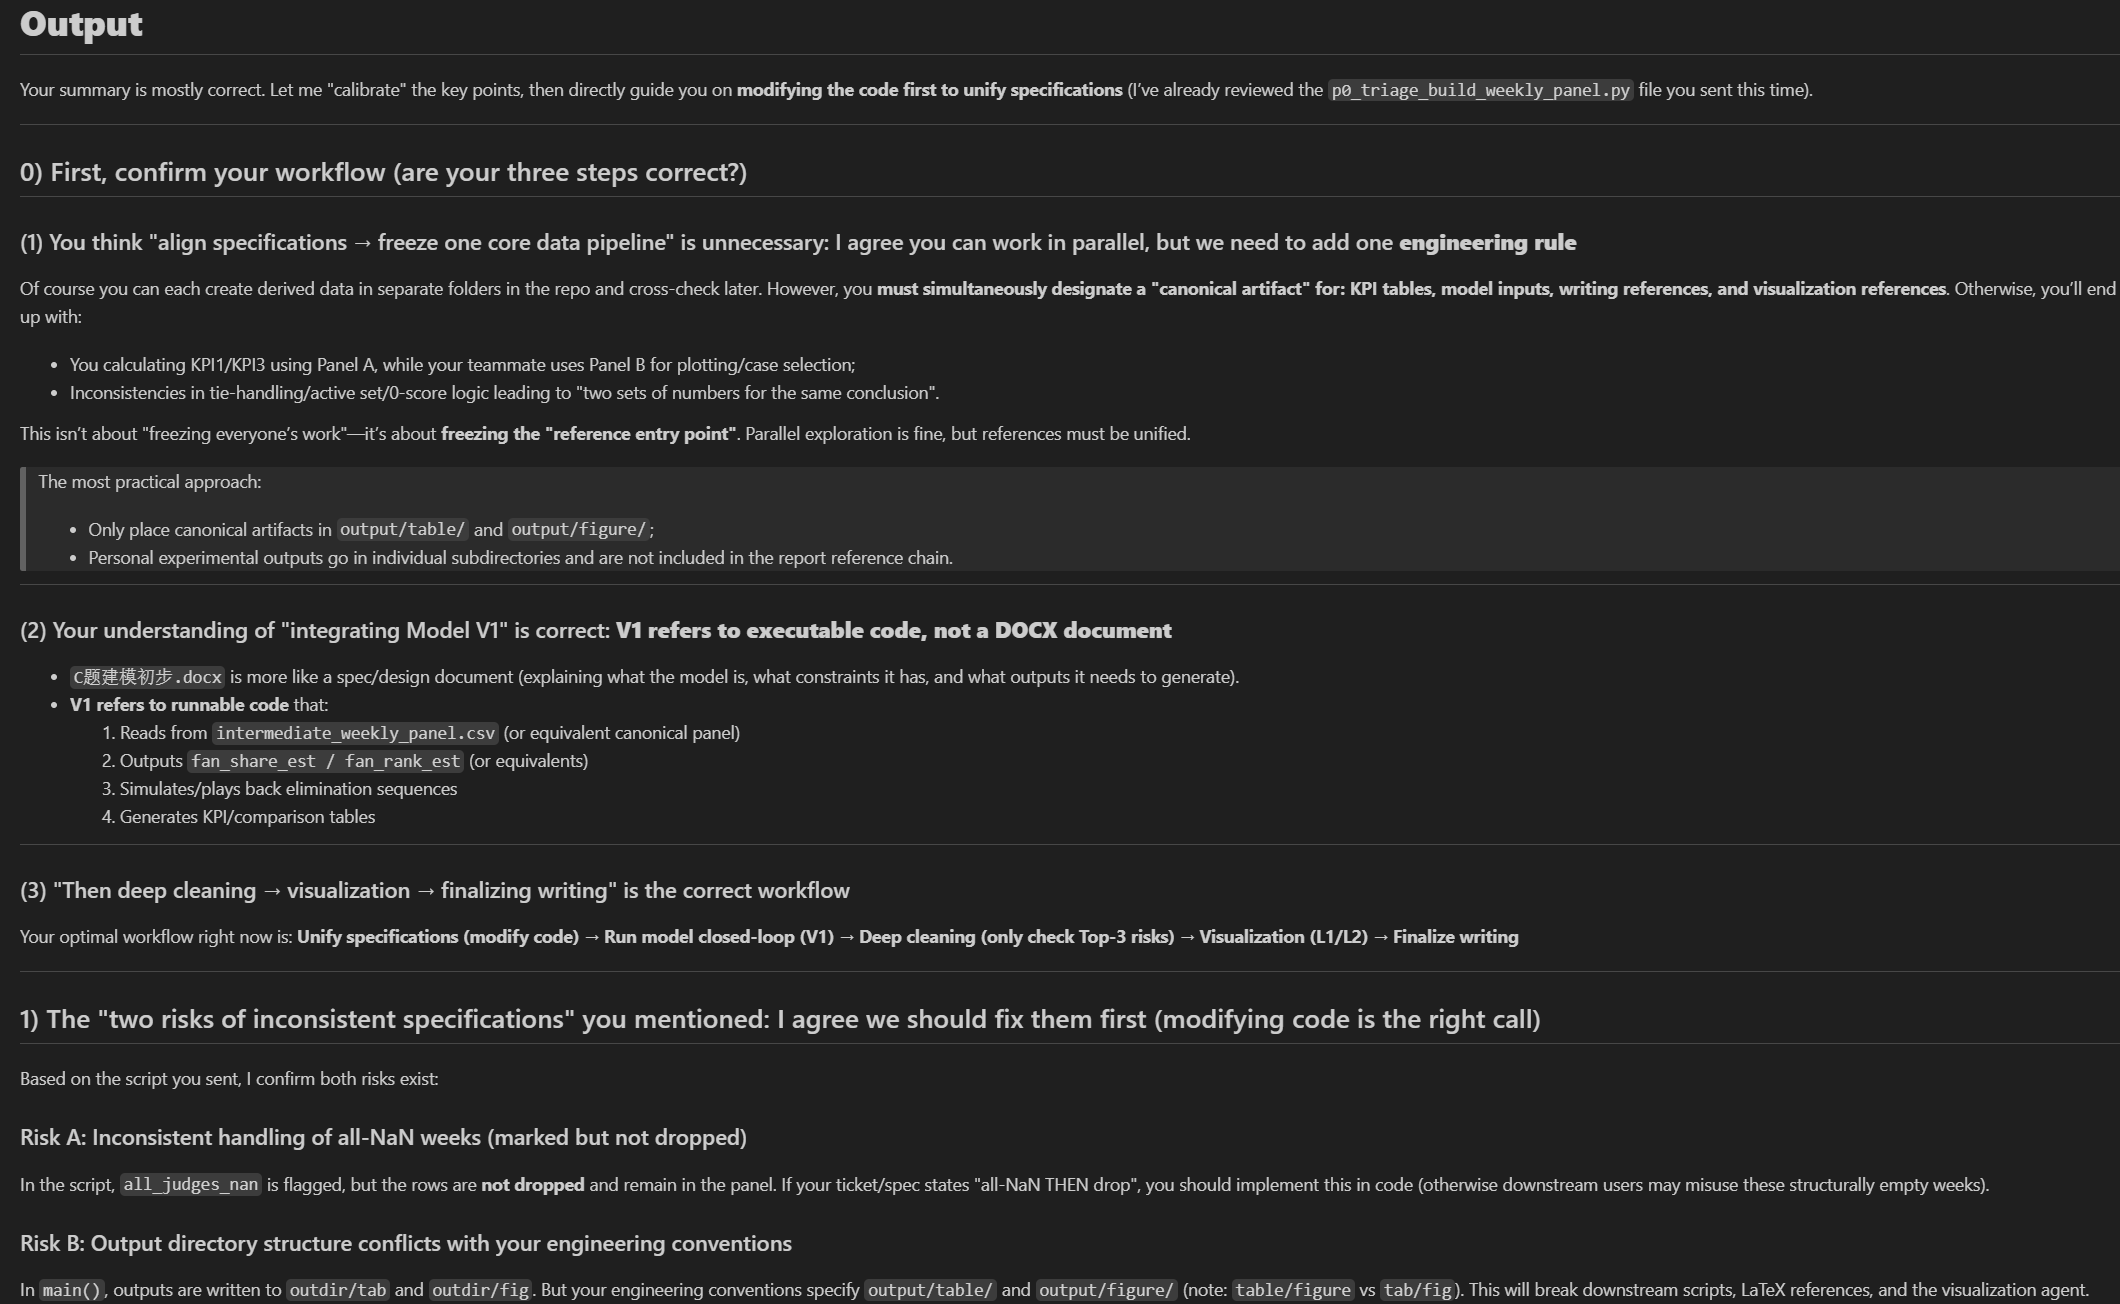
\includegraphics[width=0.9\linewidth]{report_on_use_of_ai/pho/131.png}
  \caption{ChatGPT Query 13 Output Screenshot}
  \label{fig:chatgpt_query_13_output}
\end{figure}
\begin{figure}
  \centering
  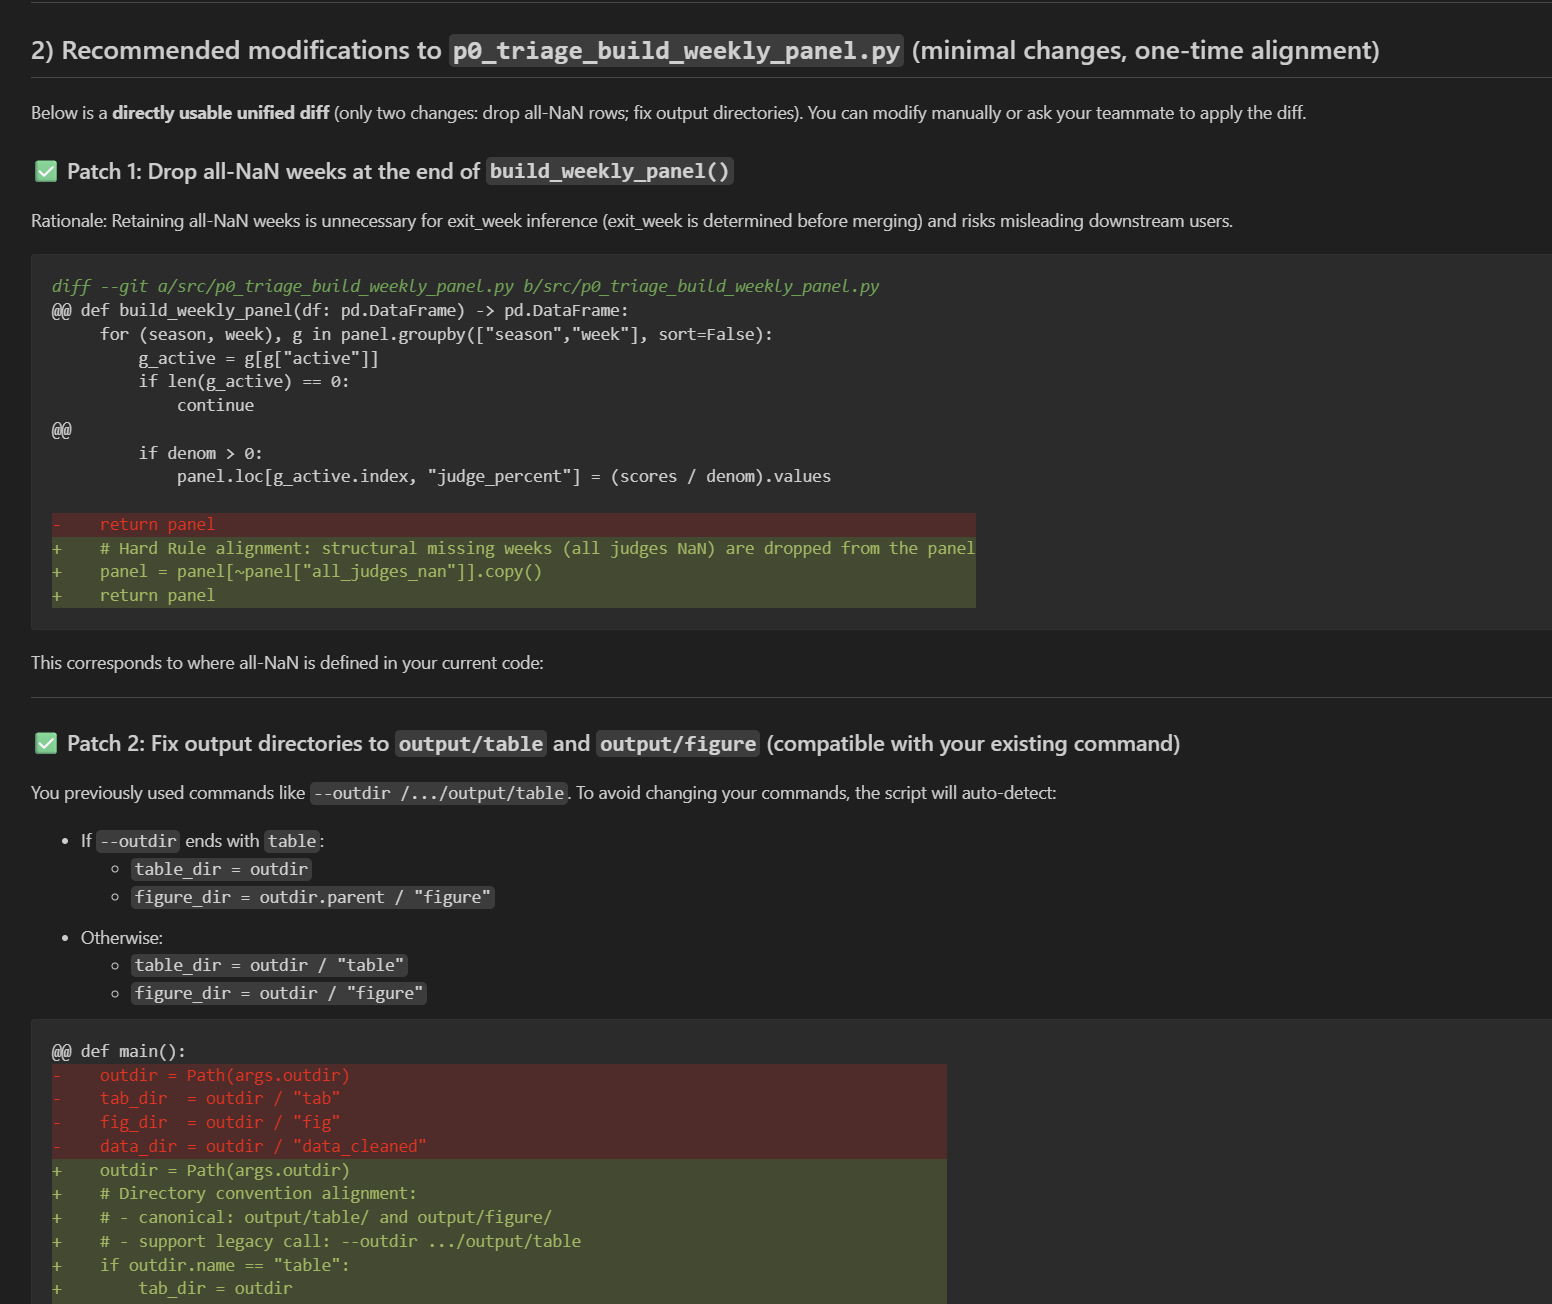
\includegraphics[width=0.9\linewidth]{report_on_use_of_ai/pho/132.png}
  \caption{ChatGPT Query 13 Output Screenshot}
  \label{fig:chatgpt_query_13_output_1}
\end{figure}
\begin{figure}
  \centering
  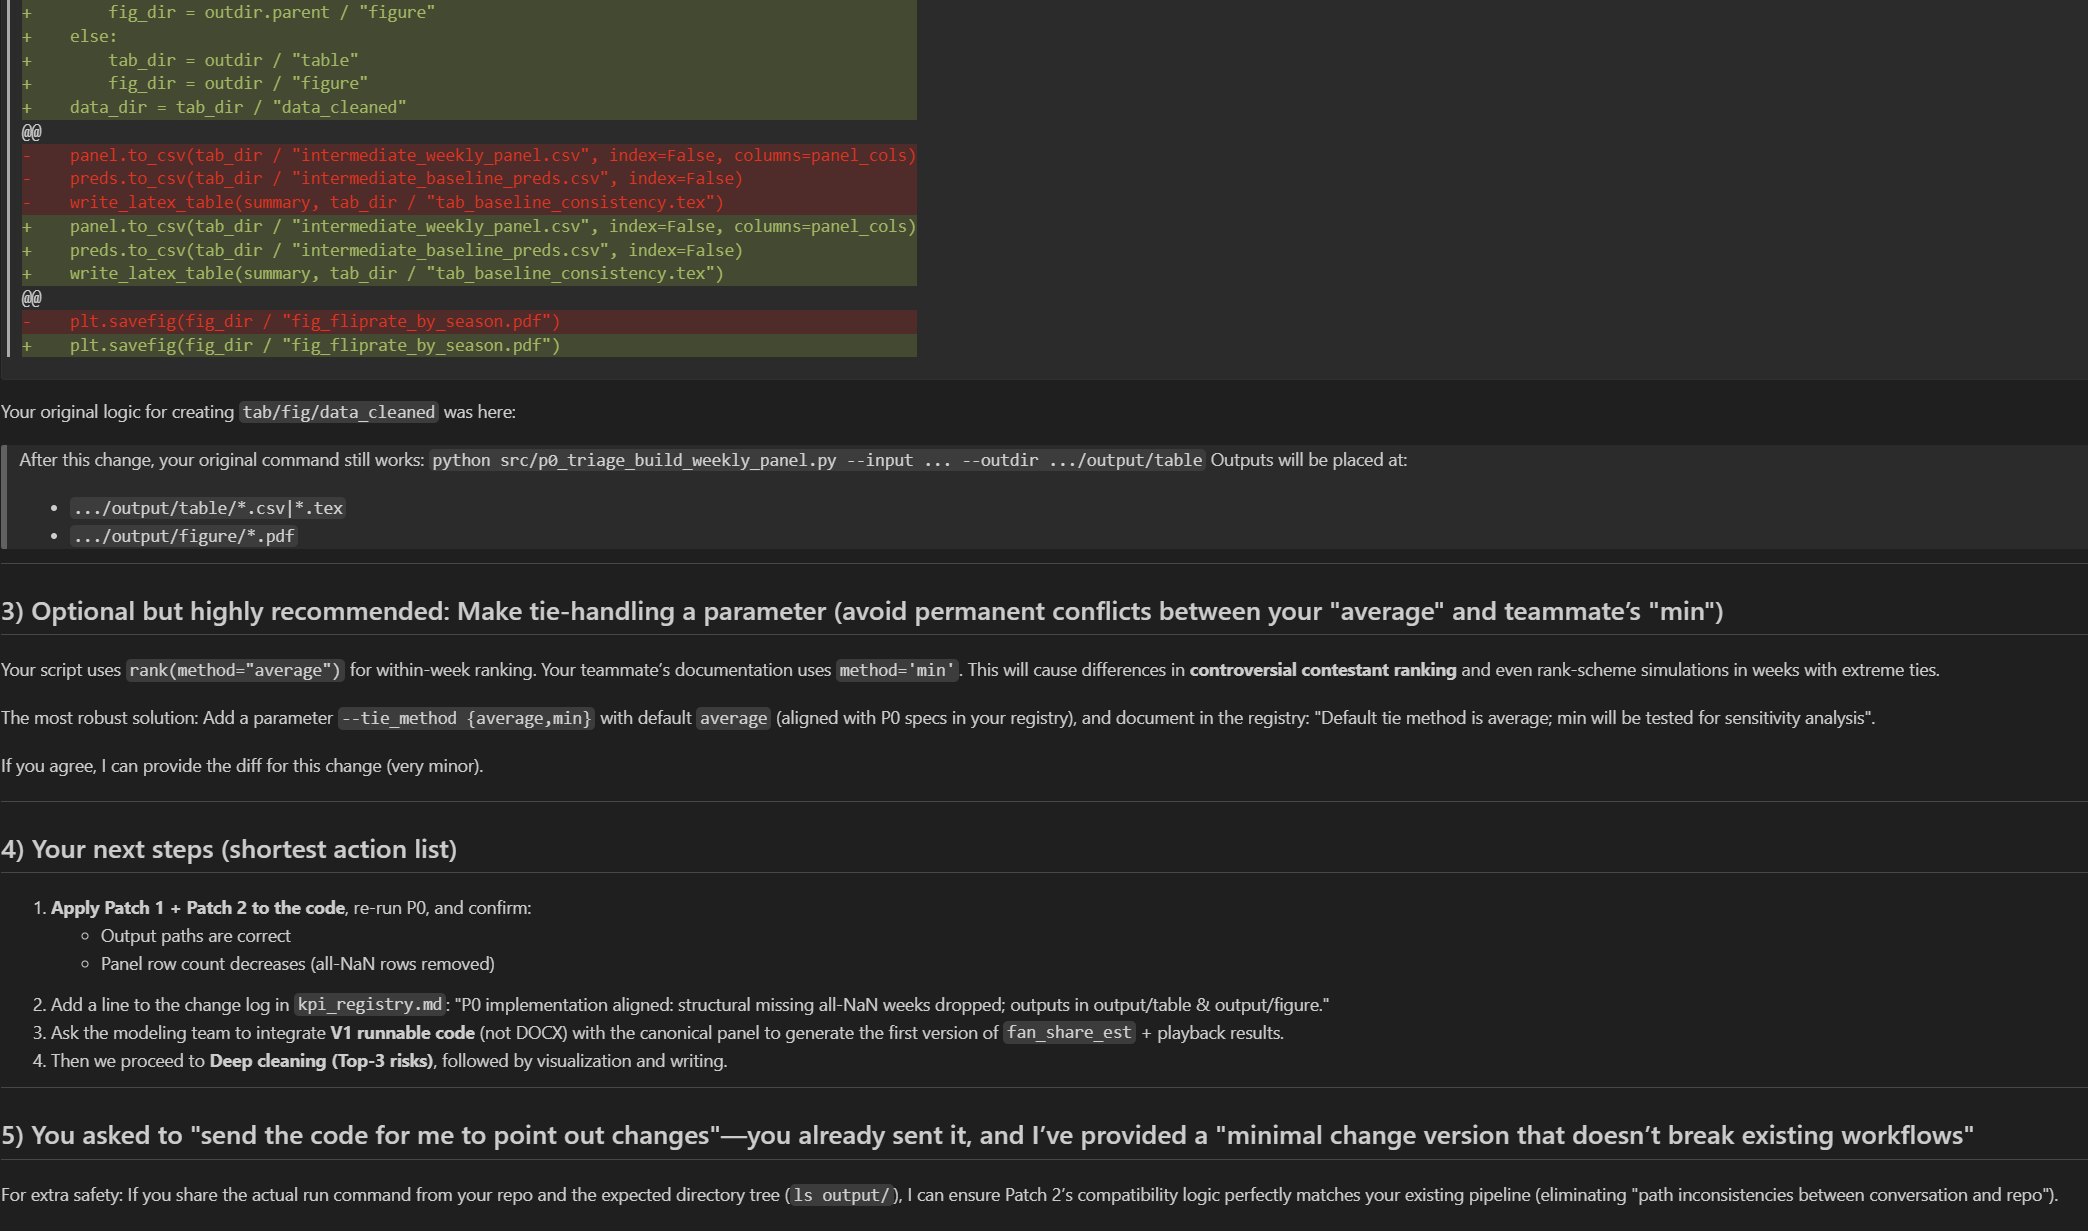
\includegraphics[width=0.9\linewidth]{report_on_use_of_ai/pho/133.png}
  \caption{ChatGPT Query 13 Output Screenshot}
  \label{fig:chatgpt_query_13_output_2}
\end{figure}




\textbf{\href{https://github.com/charles65536/model2026-2/blob/main/report_on_use_of_ai/chatgpt_14_input_and_output.md}{ChatGPT Query 14:}}\\
\textbf{Input:}
No rush, let's first sort out what we currently have:\\
1. We have the complete problem statement.\\
2. We have the preliminary data produced by our data team member just now.\\
3. We have the preliminary model developed by our modeling team member.\\
Please let me know what other files are needed and I will provide them.

Therefore, I think our workflow should be as follows:\\
1. First, complete the construction of the framework.\\
2. Then, provide you with our modeling spec, and then see which parts we can complete (my initial idea is that we can first finish the "Problem Restatement", "Key Assumptions", "Core Variables", and a bit of the beginning of the model; please supplement anything that is missing).\\
3. We will investigate the existing files and write the parts that can be included in the article.\\
\textbf{Output:}
\begin{figure}[H]
  \centering
  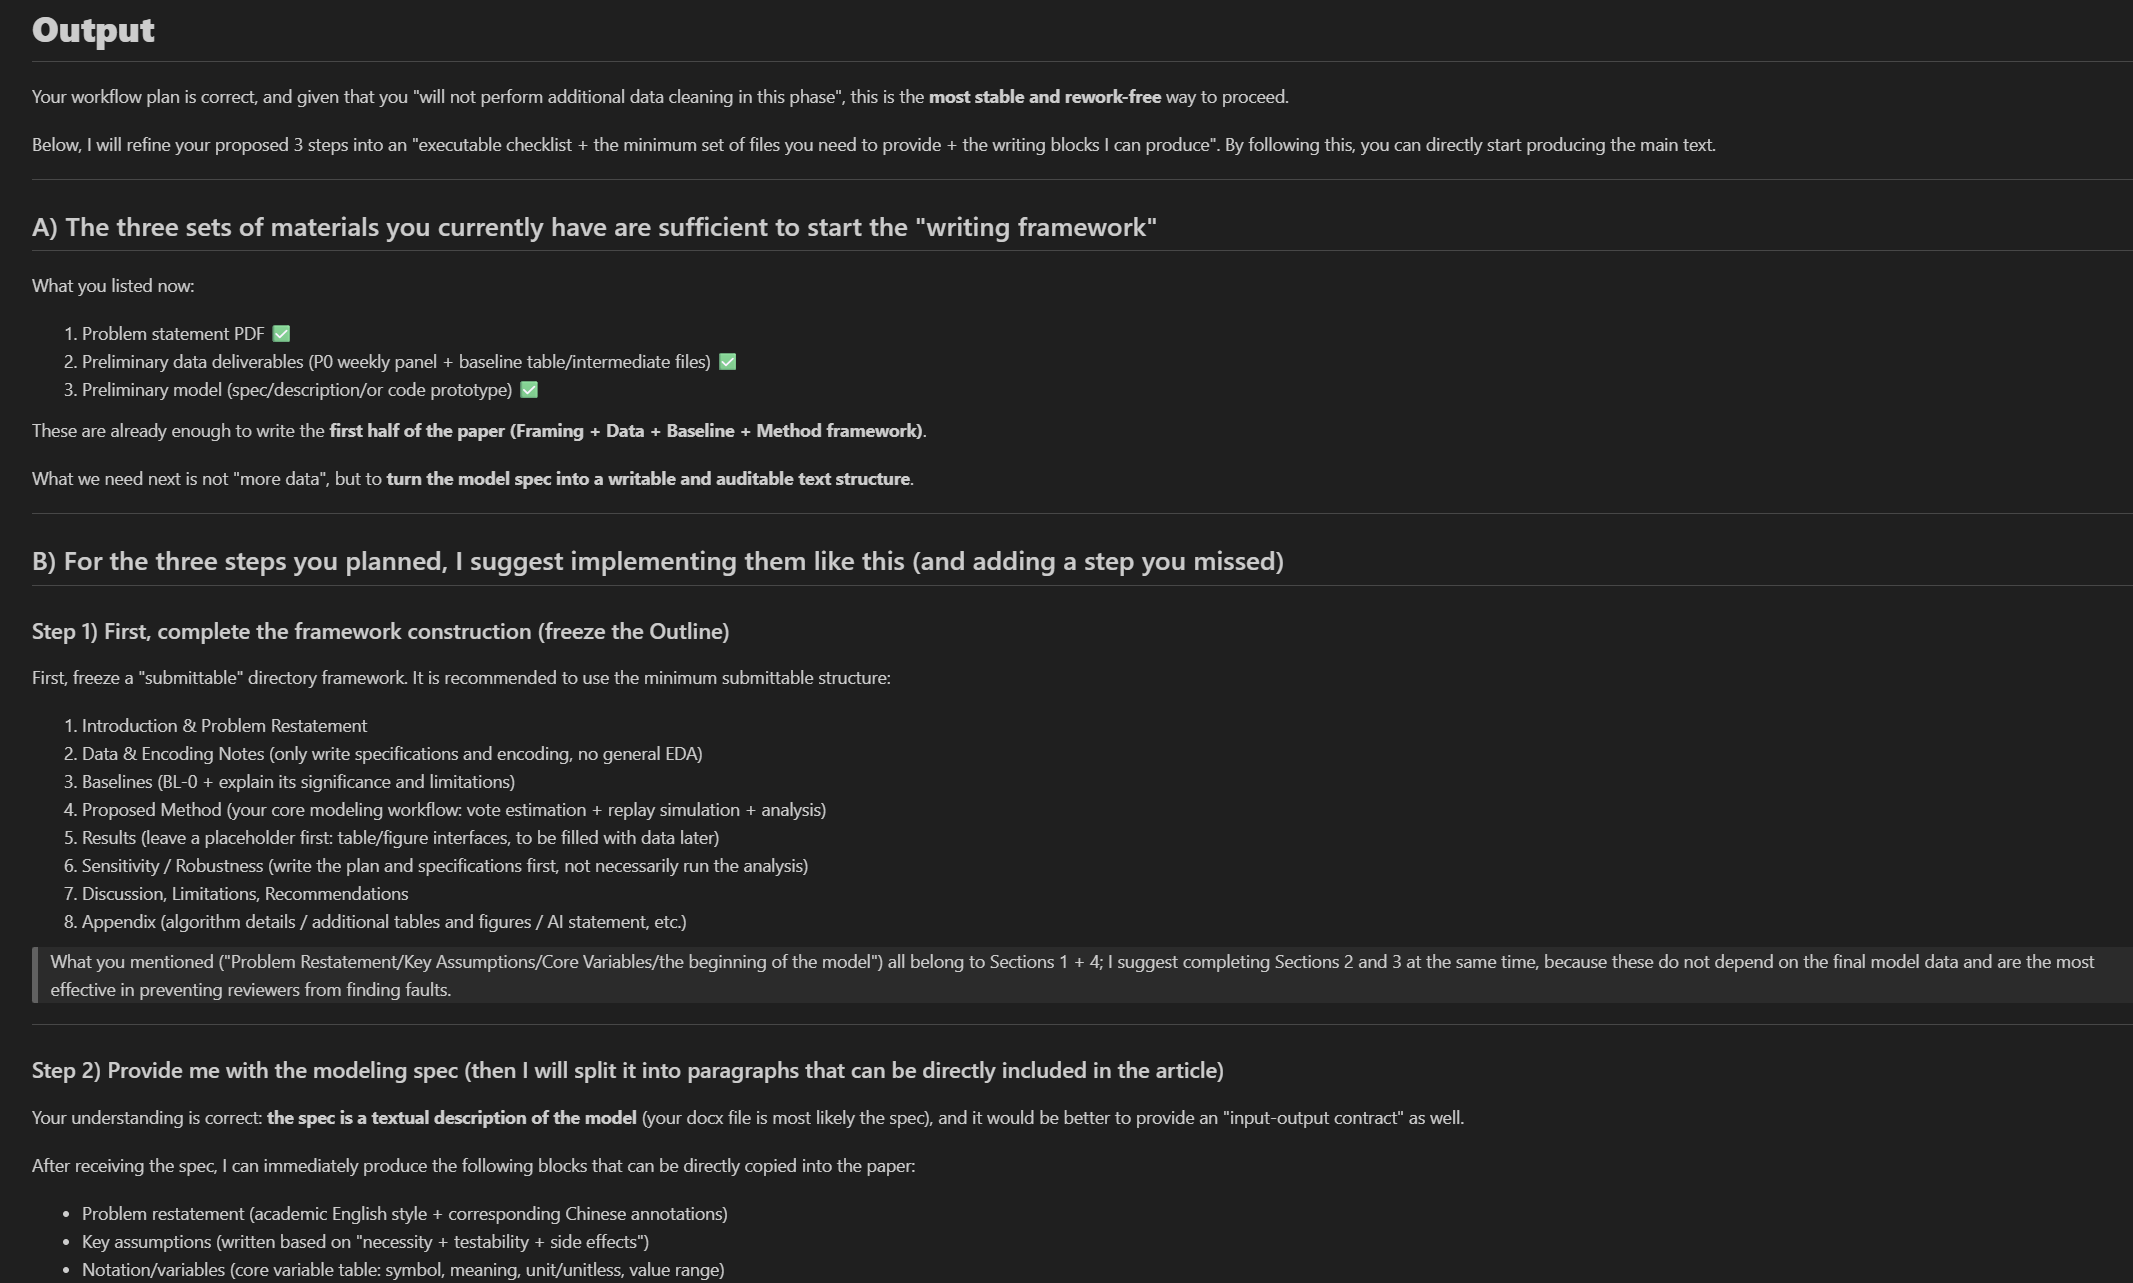
\includegraphics[width=0.9\linewidth]{report_on_use_of_ai/pho/141.png}
  \caption{ChatGPT Query 14 Output Screenshot}
  \label{fig:chatgpt_query_14_output}
\end{figure}
\begin{figure}[H]
  \centering
  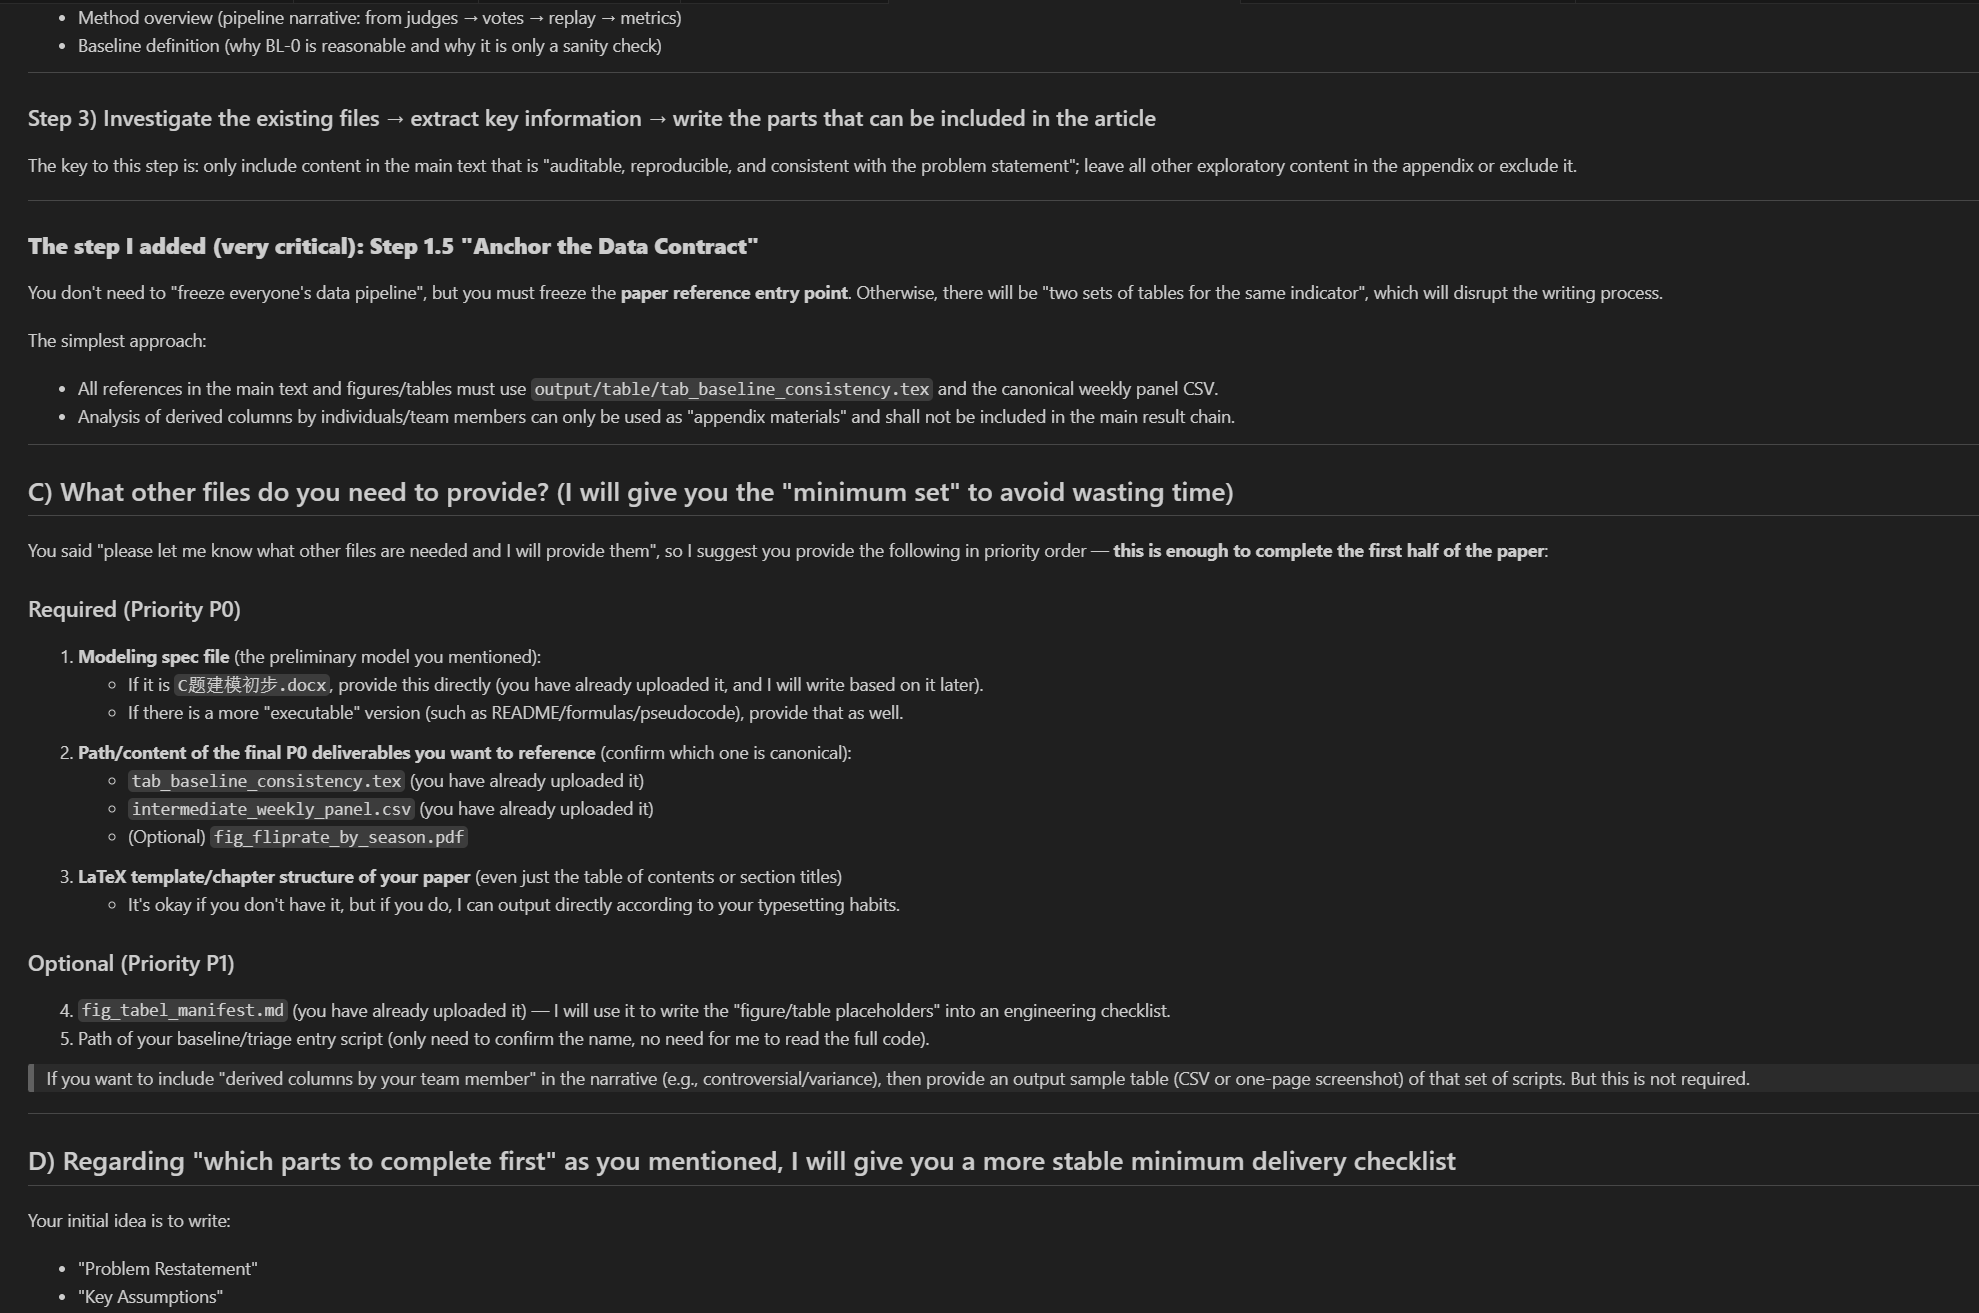
\includegraphics[width=0.9\linewidth]{report_on_use_of_ai/pho/142.png}
  \caption{ChatGPT Query 14 Output Screenshot}
  \label{fig:chatgpt_query_14_output_1}
\end{figure}
\begin{figure}[H]
  \centering
  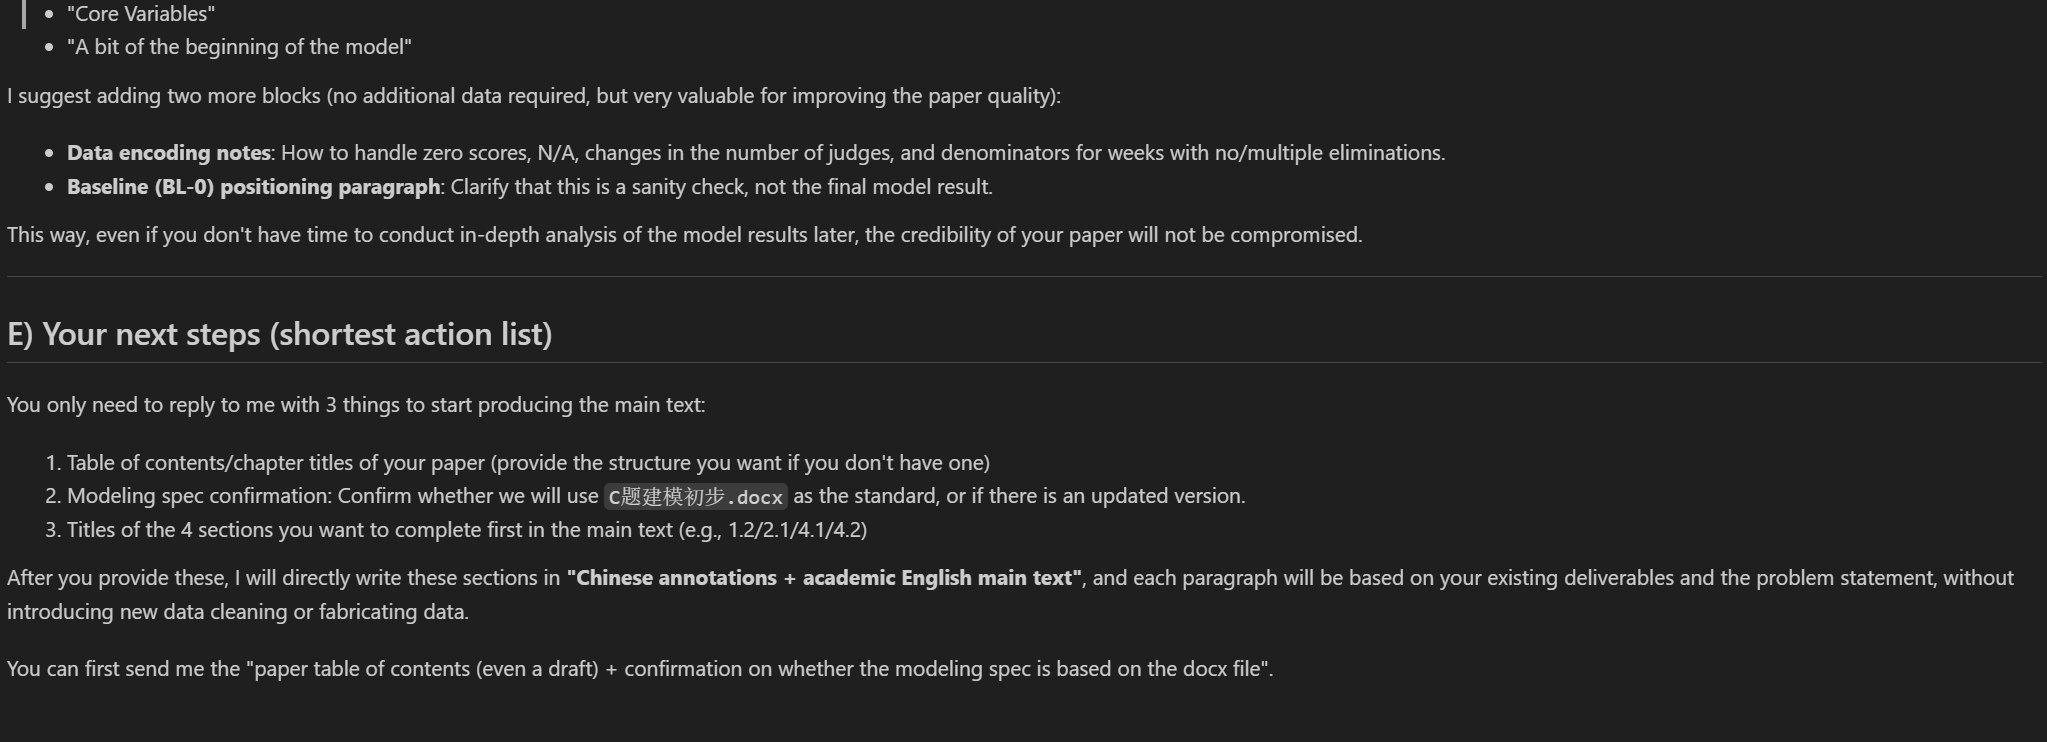
\includegraphics[width=0.9\linewidth]{report_on_use_of_ai/pho/143.png}
  \caption{ChatGPT Query 14 Output Screenshot}
  \label{fig:chatgpt_query_14_output_2}
\end{figure}



\subsection*{\center{Human Contribution Declaration}}
We affirm that:
\begin{enumerate}
  \item All final modeling decisions, algorithm designs, and strategic choices were made by the team members.
  \item All mathematical formulations and assumptions were independently derived or verified by the team.
  \item All code included in this project was reviewed, tested, and fully understood by the team.
  \item AI tools were used only for brainstorming, drafting, language refinement, and preliminary coding assistance.
  \item The submitted work represents our own understanding and intellectual contribution.
\end{enumerate}
\begin{flushright}
Date: Feb 2, 2026
\end{flushright}
\normalsize
\endgroup
\end{document}